\documentclass{article}

% For submission
\usepackage[preprint]{neurips_2025}

\usepackage[utf8]{inputenc}
\usepackage[T1]{fontenc}
\usepackage{hyperref}
\usepackage{url}
\usepackage{booktabs}
\usepackage{amsfonts}
\usepackage{nicefrac}
\usepackage{microtype}
\usepackage{xcolor}


\usepackage{float}
\usepackage{multirow}
\usepackage{amsmath}
\usepackage{amssymb}
\usepackage{subcaption}
\usepackage{graphicx}
\title{
    Computer Vision Final Project Report
}

\author{
    Ming Cheng \\
    23307130007
    \And
    Yifan Luo \\
    23307130031
}

\begin{document}

\maketitle

\begin{abstract}
This report presents two computer vision and embodied AI tasks.

The first task focuses on neural rendering and AIGC-based 3D reconstruction and generation, including real-world multi-view reconstruction, text-to-3D generation, single-image-to-3D generation, and scene fusion rendering. COLMAP, 2D Gaussian Splatting (2DGS), and the pre-trained DREAMFUSION-IF and Magic123 frameworks in threestudio are utilized to construct a complete 3D vision pipeline. After reconstruction, they were exported as textured meshes and then combined in Blender.

The second task investigates the zero-shot cross-environment generalization of Action Chunking with Transformers (ACT) on the CALVIN benchmark. Experimental results show that multi-environment training substantially improves robustness to visual distribution shifts, reducing the Action $L_1$ Error on an unseen environment by 15.7\% and increasing the rollout success rate from 0\% to 100\%. Furthermore, an ablation study demonstrates that moderate action horizons consistently yield the best performance.

\end{abstract}

\section*{Team Contribution}

This project was completed collaboratively by Yifan Luo and Ming Cheng. Both authors contributed to project discussion, experimental design, implementation, result analysis, and report writing.

\section{Introduction}

Recent advances in 3D vision and robot learning have significantly expanded the capabilities of embodied intelligent systems. On one hand, neural rendering and 3D generation techniques enable the reconstruction of realistic virtual environments from images. On the other hand, learning-based manipulation policies allow robots to acquire complex skills directly from demonstrations. Together, these developments provide a foundation for building interactive virtual worlds and autonomous robotic systems that can perceive and act in complex environments.

This project consists of two complementary tasks. The first task focuses on 3D reconstruction and scene generation. Multiple objects and background components are reconstructed using a combination of multi-view reconstruction and image-guided 3D generation methods, and the resulting assets are integrated into a complete virtual scene. The second task investigates the cross-environment generalization ability of robotic manipulation policies. Specifically, we evaluate whether Action Chunking with Transformers (ACT) can successfully transfer to visually different environments under a zero-shot setting.

In Task 1, several 3D assets are reconstructed. For Object A and the background, we use COLMAP for camera pose estimation combined with 2D Gaussian Splatting (2DGS) to exploit multi-view geometric consistency. For Objects B and C, we leverage threestudio and Magic123 for image-guided 3D generation. We analyze training dynamics through loss curves and evaluate reconstruction quality using standard metrics including SSIM, PSNR, LPIPS, and training time. Finally, the reconstructed assets are exported as textured meshes and integrated into a complete scene in Blender.

In Task 2, we study the zero-shot transfer capability of ACT on the CALVIN benchmark under substantial visual distribution shifts. Policies are trained using demonstrations collected from one or multiple environments and subsequently evaluated on a previously unseen environment. We assess policy performance using both offline action prediction metrics and online rollout success rates, and further investigate the influence of multi-environment training and action chunking on cross-environment generalization.


\section{Task 1: 3D Resources Reconstruction and Real Scene Fusion}

In this task,for multi-view real-world reconstruction, COLMAP and Gaussian Splatting are applied to reconstruct a physical object captured by mobile-phone images from multiple viewpoints; for text-driven 3D generation, the threestudio framework is explored with score distillation sampling (SDS) and pretrained diffusion priors to synthesize a virtual 3D asset from text prompts; for single-image 3D generation, Magic123 is employed to generate a textured 3D model from a single foreground image. In addition, a large-scale background scene is reconstructed using Gaussian Splatting and integrated with the generated assets in a unified 3D environment in Blender.


\subsection{Dataset and Data Preprocessing}
Due to the requirements of this task, most of the dataset is filmed by smartphone, with the same resolution of 3456*4608. As for the scene construction, the \textbf{"garden"} dataset is collected form the Mip-NeRF 360 dataset.

For the smartphone captured dataset, \textbf{87} images of a Kobe's clay sculpture are collected from multiple viewpoints including horizontal, high-angle, and low-angle trajectories to ensure sufficient geometric coverage; one image of a cute astronaut robot is shot from a front to cover most of its features. Specifically, for Object C, the background was removed, and the foreground object was extracted. We also tried a picture given by the threestudio. These will be showed later.  
\subsection{Training Pipeline}
In this part, the training pipeline of different 3D resources are introduced.

To specify, the whole experimental environment is built upon a single NVIDIA GeForce RTX 4090 GPU, which features 24 GB memory. The processing unit comprises 20 virtual CPU cores (vCPUs) allocated from an Intel Xeon Platinum 8470Q server processor, while the system is supplemented with 90 GB of available random-access memory to accommodate large-scale data loading and computational overheads during training and inference from \textbf{AutoDL}
\subsubsection{Object A}
The real-world multi-view object is implemented based on the 2DGS framework, which consists of 2 major stages: camera pose estimation, and Gaussian Splatting optimization.

First, COLMAP is used to perform structure-from-motion (SfM) reconstruction and estimate camera intrinsics and extrinsics. Sparse point clouds and camera poses generated by COLMAP are then used to initialize the Gaussian representation.

Then, the reconstructed scene is optimized using the official Gaussian Splatting framework, which generates the original point cloud.



\subsubsection{Object B}
The text-driven 3D asset generation task is implemented based on the \textit{threestudio} framework, which adopts the newly-released T2I model DeepFloyd IF and SDS loss. Given a textual prompt, the framework initializes a learnable 3D representation and iteratively optimizes it by minimizing the discrepancy between rendered views and diffusion-guided image priors.

Specifically, a pretrained text-to-image diffusion model provides semantic guidance during optimization. At each iteration, SDS loss is computed to encourage consistency with the textual description.

\subsubsection{Object C}
The single-image 3D generation task is implemented using the Magic123 framework, which consists of coarse geometry initialization, diffusion-guided optimization.

First,a Neural Radiance Field (NeRF) is optimized from scratch using the input RGBA image and a text prompt describing the object.

Then,the coarse NeRF is first converted into a textured mesh via a differentiable marching tetrahedra (DMTet) representation, using a density threshold to extract the surface.
Starting from this initialization, the mesh geometry and texture are further refined with the same Zero123 and Stable Diffusion guidance.
\subsection{Single Object Visualization}

\subsubsection{Object A}
In this section, 87 pictures of Kobe, filmed from different viewpoints, are trained. It takes about \textbf{2min} to extract pose with COLMAP and \textbf{52:11min}(20000 epochs) to train.

One of the original pictures and the rendering results are as follow(the training dynamics will be posed later with the background scene):


\begin{figure}[H]
	\centering
	

	\begin{subfigure}{0.25\textwidth}
		\centering
		\includegraphics[width=\linewidth]{figures/task1/objectA/Kobe_mesh.png}
		\caption{Kobe Mesh(Floating points and background are manually eliminated)}
	\end{subfigure}
	\hfill
	\begin{subfigure}{0.25\textwidth}
		\centering
		\includegraphics[width=\linewidth]{figures/task1/objectA/Kobe_color.png}
		\caption{Kobe Color}
	\end{subfigure}
	\hfill
	\begin{subfigure}{0.25\textwidth}
		\centering
		\includegraphics[width=\linewidth]{figures/task1/objectA/original_Kobe.jpg}
		\caption{Original Kobe}
	\end{subfigure}
\end{figure}

We can see that the reconstruction has a relatively good fit, the detailed quality analysis will be shown later in Figure~\ref{fig:2DGS Dynamics}

\subsubsection{Object B}
In this section, 2 examples are trained, the prompt are as follow:
\begin{itemize}
	\item A zoomed-out DSLR photo of a baby bunny sitting on top of a stack of pancakes.
	\item A Michelangelo-style statue of an astronaut.
\end{itemize}

Each training takes about \textbf{20 minutes}(10000 epochs), the rendering results and training dynamics are as follow:

\begin{figure}[H]
	\centering
	
	%================ 第一组：Astronaut =================
	\begin{subfigure}{0.25\textwidth}
		\centering
		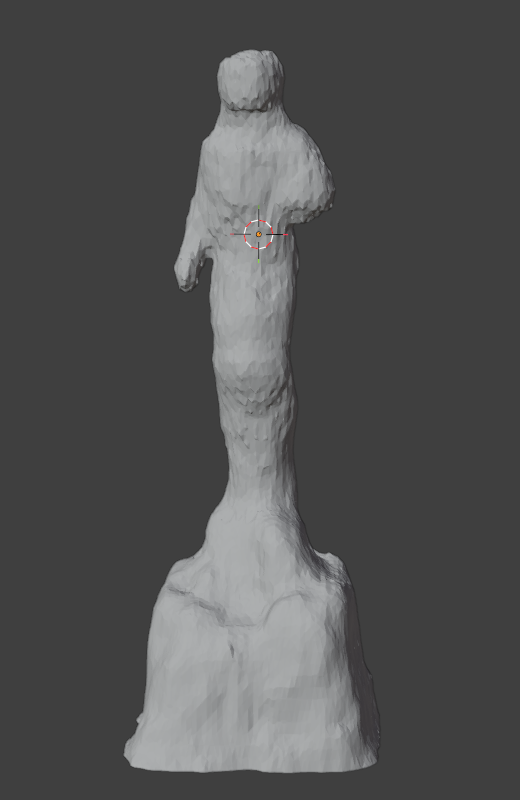
\includegraphics[width=\linewidth]{figures/task1/objectB/astronaut_mesh.png}
		\caption{Astronaut Mesh}
	\end{subfigure}
	\hfill
	\begin{subfigure}{0.25\textwidth}
		\centering
		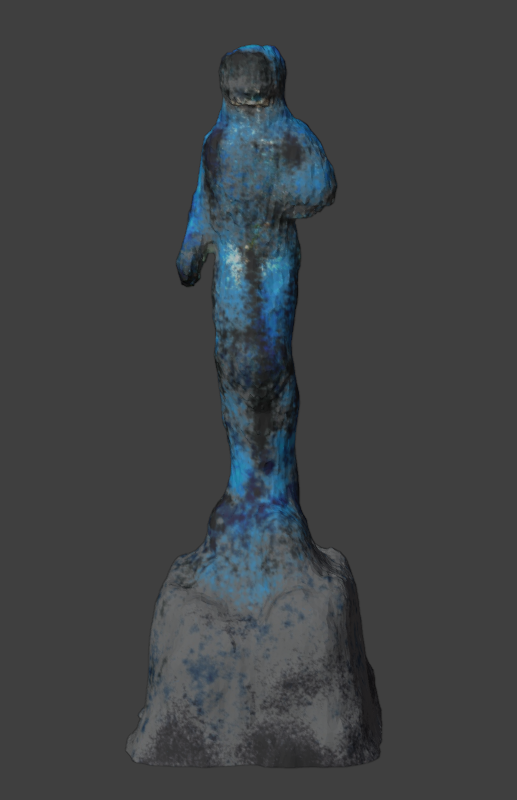
\includegraphics[width=\linewidth]{figures/task1/objectB/astronaut_color.png}
		\caption{Astronaut Color}
		\label{Astronaut Color}
	\end{subfigure}
	\hfill
	\begin{subfigure}{0.25\textwidth}
		\centering
		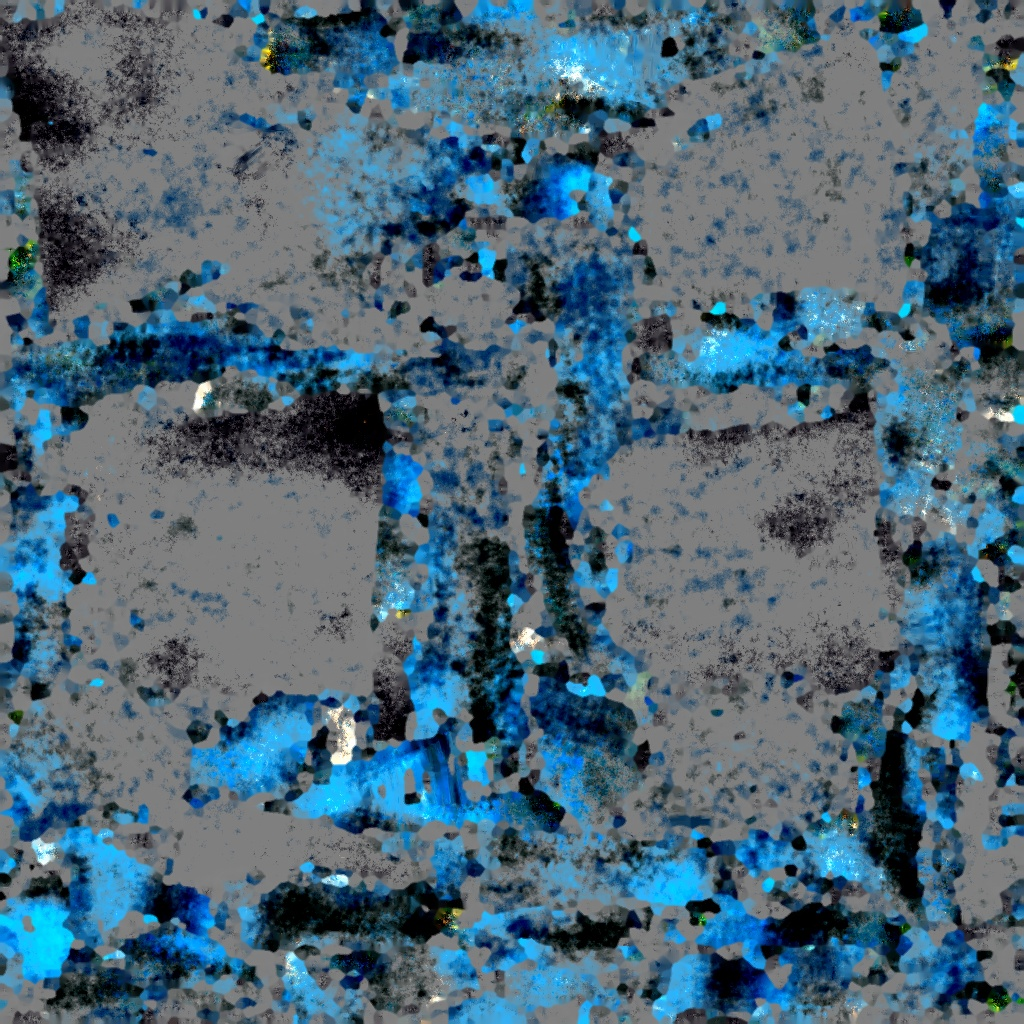
\includegraphics[width=\linewidth]{figures/task1/objectB/astronaut_texture_kd.jpg}
		\caption{Astronaut Texture}
	\end{subfigure}
	
	\vspace{0.6cm}
	
	%================ 第二组：Bunny =================
		% 第一张图（左边）
	\begin{subfigure}{0.8\textwidth}
		\centering
		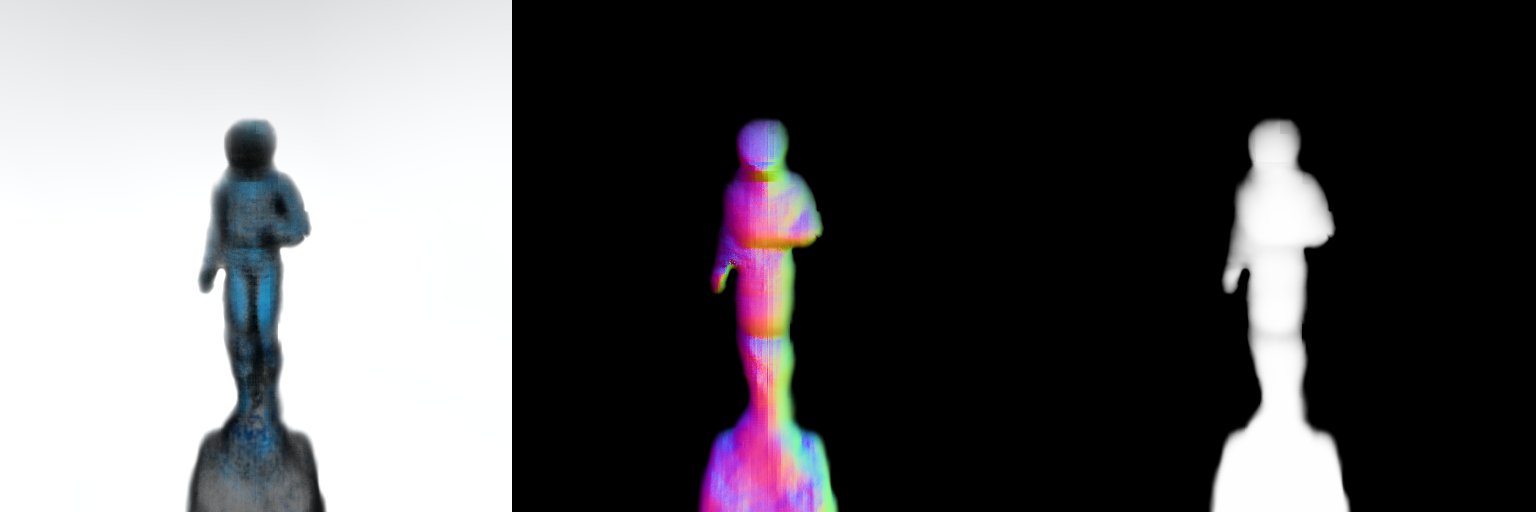
\includegraphics[width=\linewidth]{figures/task1/objectB/astronauts.png} % 替换为你的第一张图片路径
		\caption{Astronauts} % 替换为你想要的图注
	\end{subfigure}
	\hfill % 左右两张图之间的弹性间距

\end{figure}



\begin{figure}[H]
		\begin{subfigure}{0.25\textwidth}
		\centering
		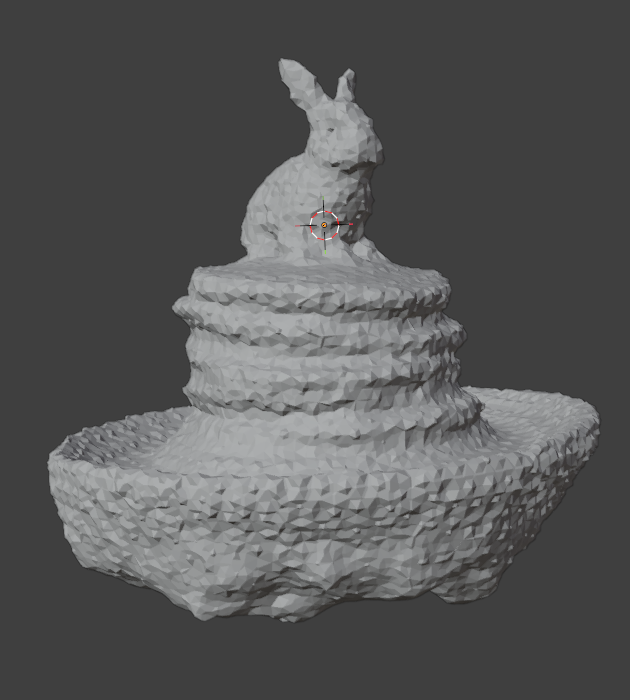
\includegraphics[width=\linewidth]{figures/task1/objectB/bunny_mesh.png}
		\caption{Bunny Mesh}
	\end{subfigure}
	\hfill
	\begin{subfigure}{0.25\textwidth}
		\centering
		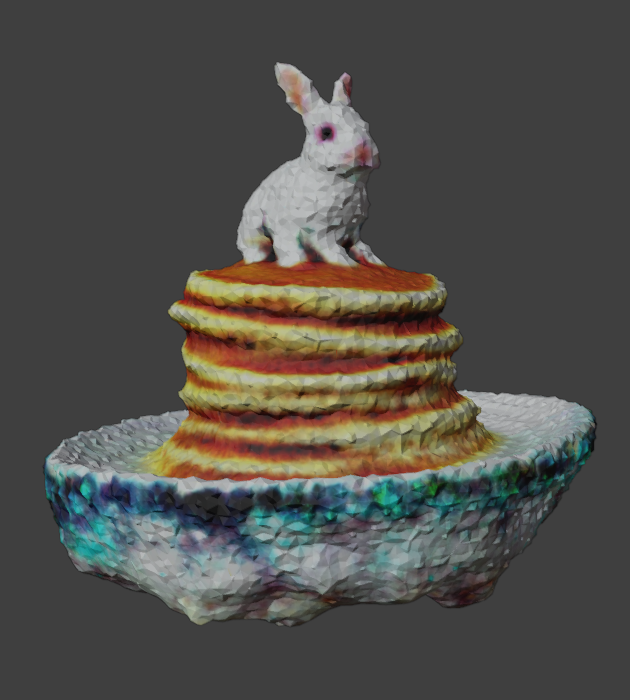
\includegraphics[width=\linewidth]{figures/task1/objectB/bunny_color.png}
		\caption{Bunny Color}
	\end{subfigure}
	\hfill
	\begin{subfigure}{0.25\textwidth}
		\centering
		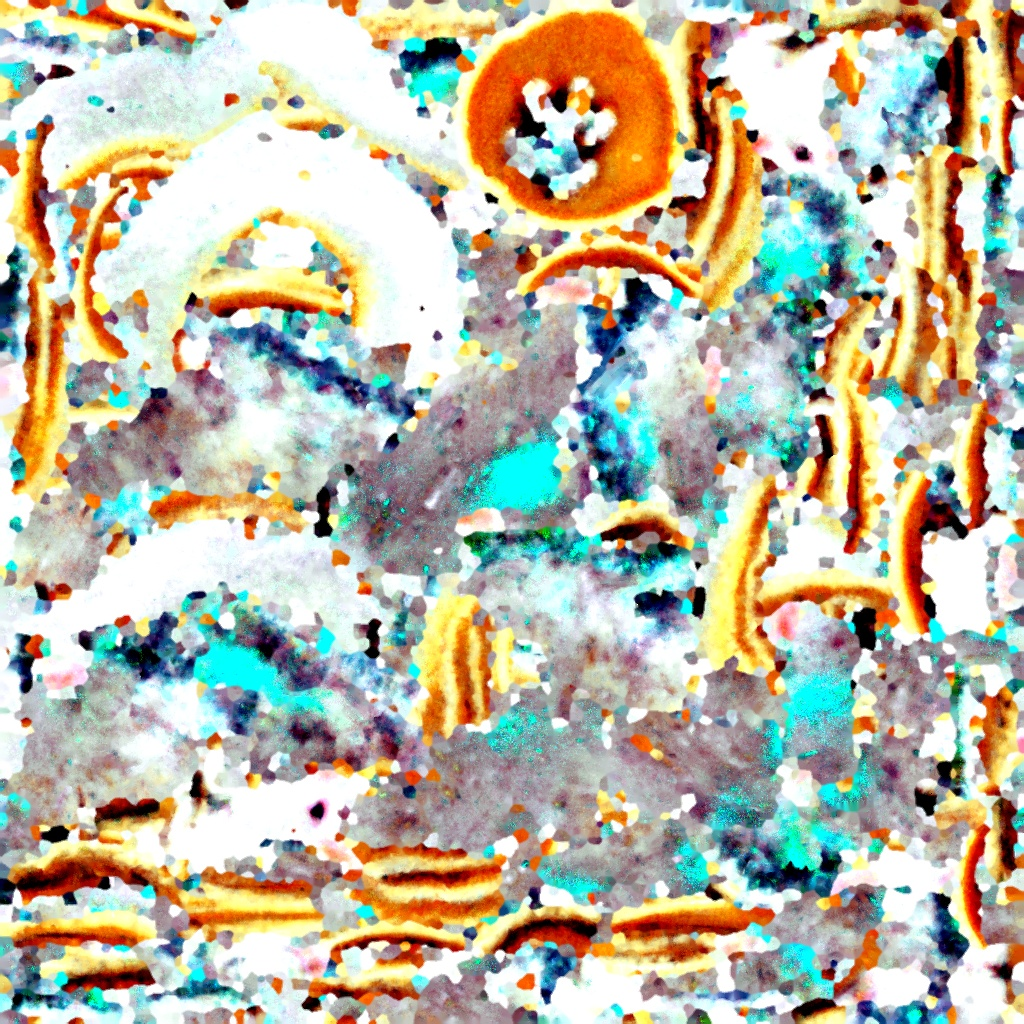
\includegraphics[width=\linewidth]{figures/task1/objectB/bunny_texture_kd.jpg}
		\caption{Bunny Texture}
	\end{subfigure}
	
	\centering
	\vspace{0.6cm}

	% 第二张图（右边）
	\begin{subfigure}{0.8\textwidth}
		\centering
		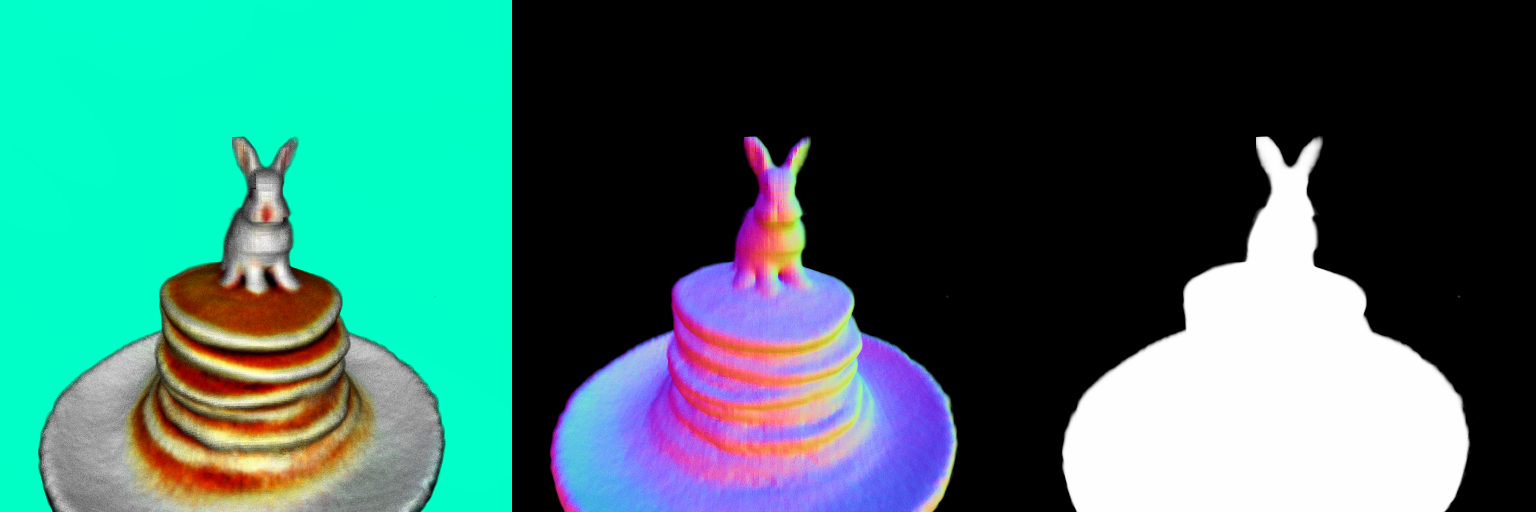
\includegraphics[width=\linewidth]{figures/task1/objectB/bunnys.png} % 替换为你的第二张图片路径
		\caption{Bunnys} % 替换为你想要的图注
	\end{subfigure}

\end{figure}


%================ Loss Functions =================
\begin{figure}[H]
	\centering
	
	% 第一行
	\begin{subfigure}{0.4\textwidth}
		\centering
		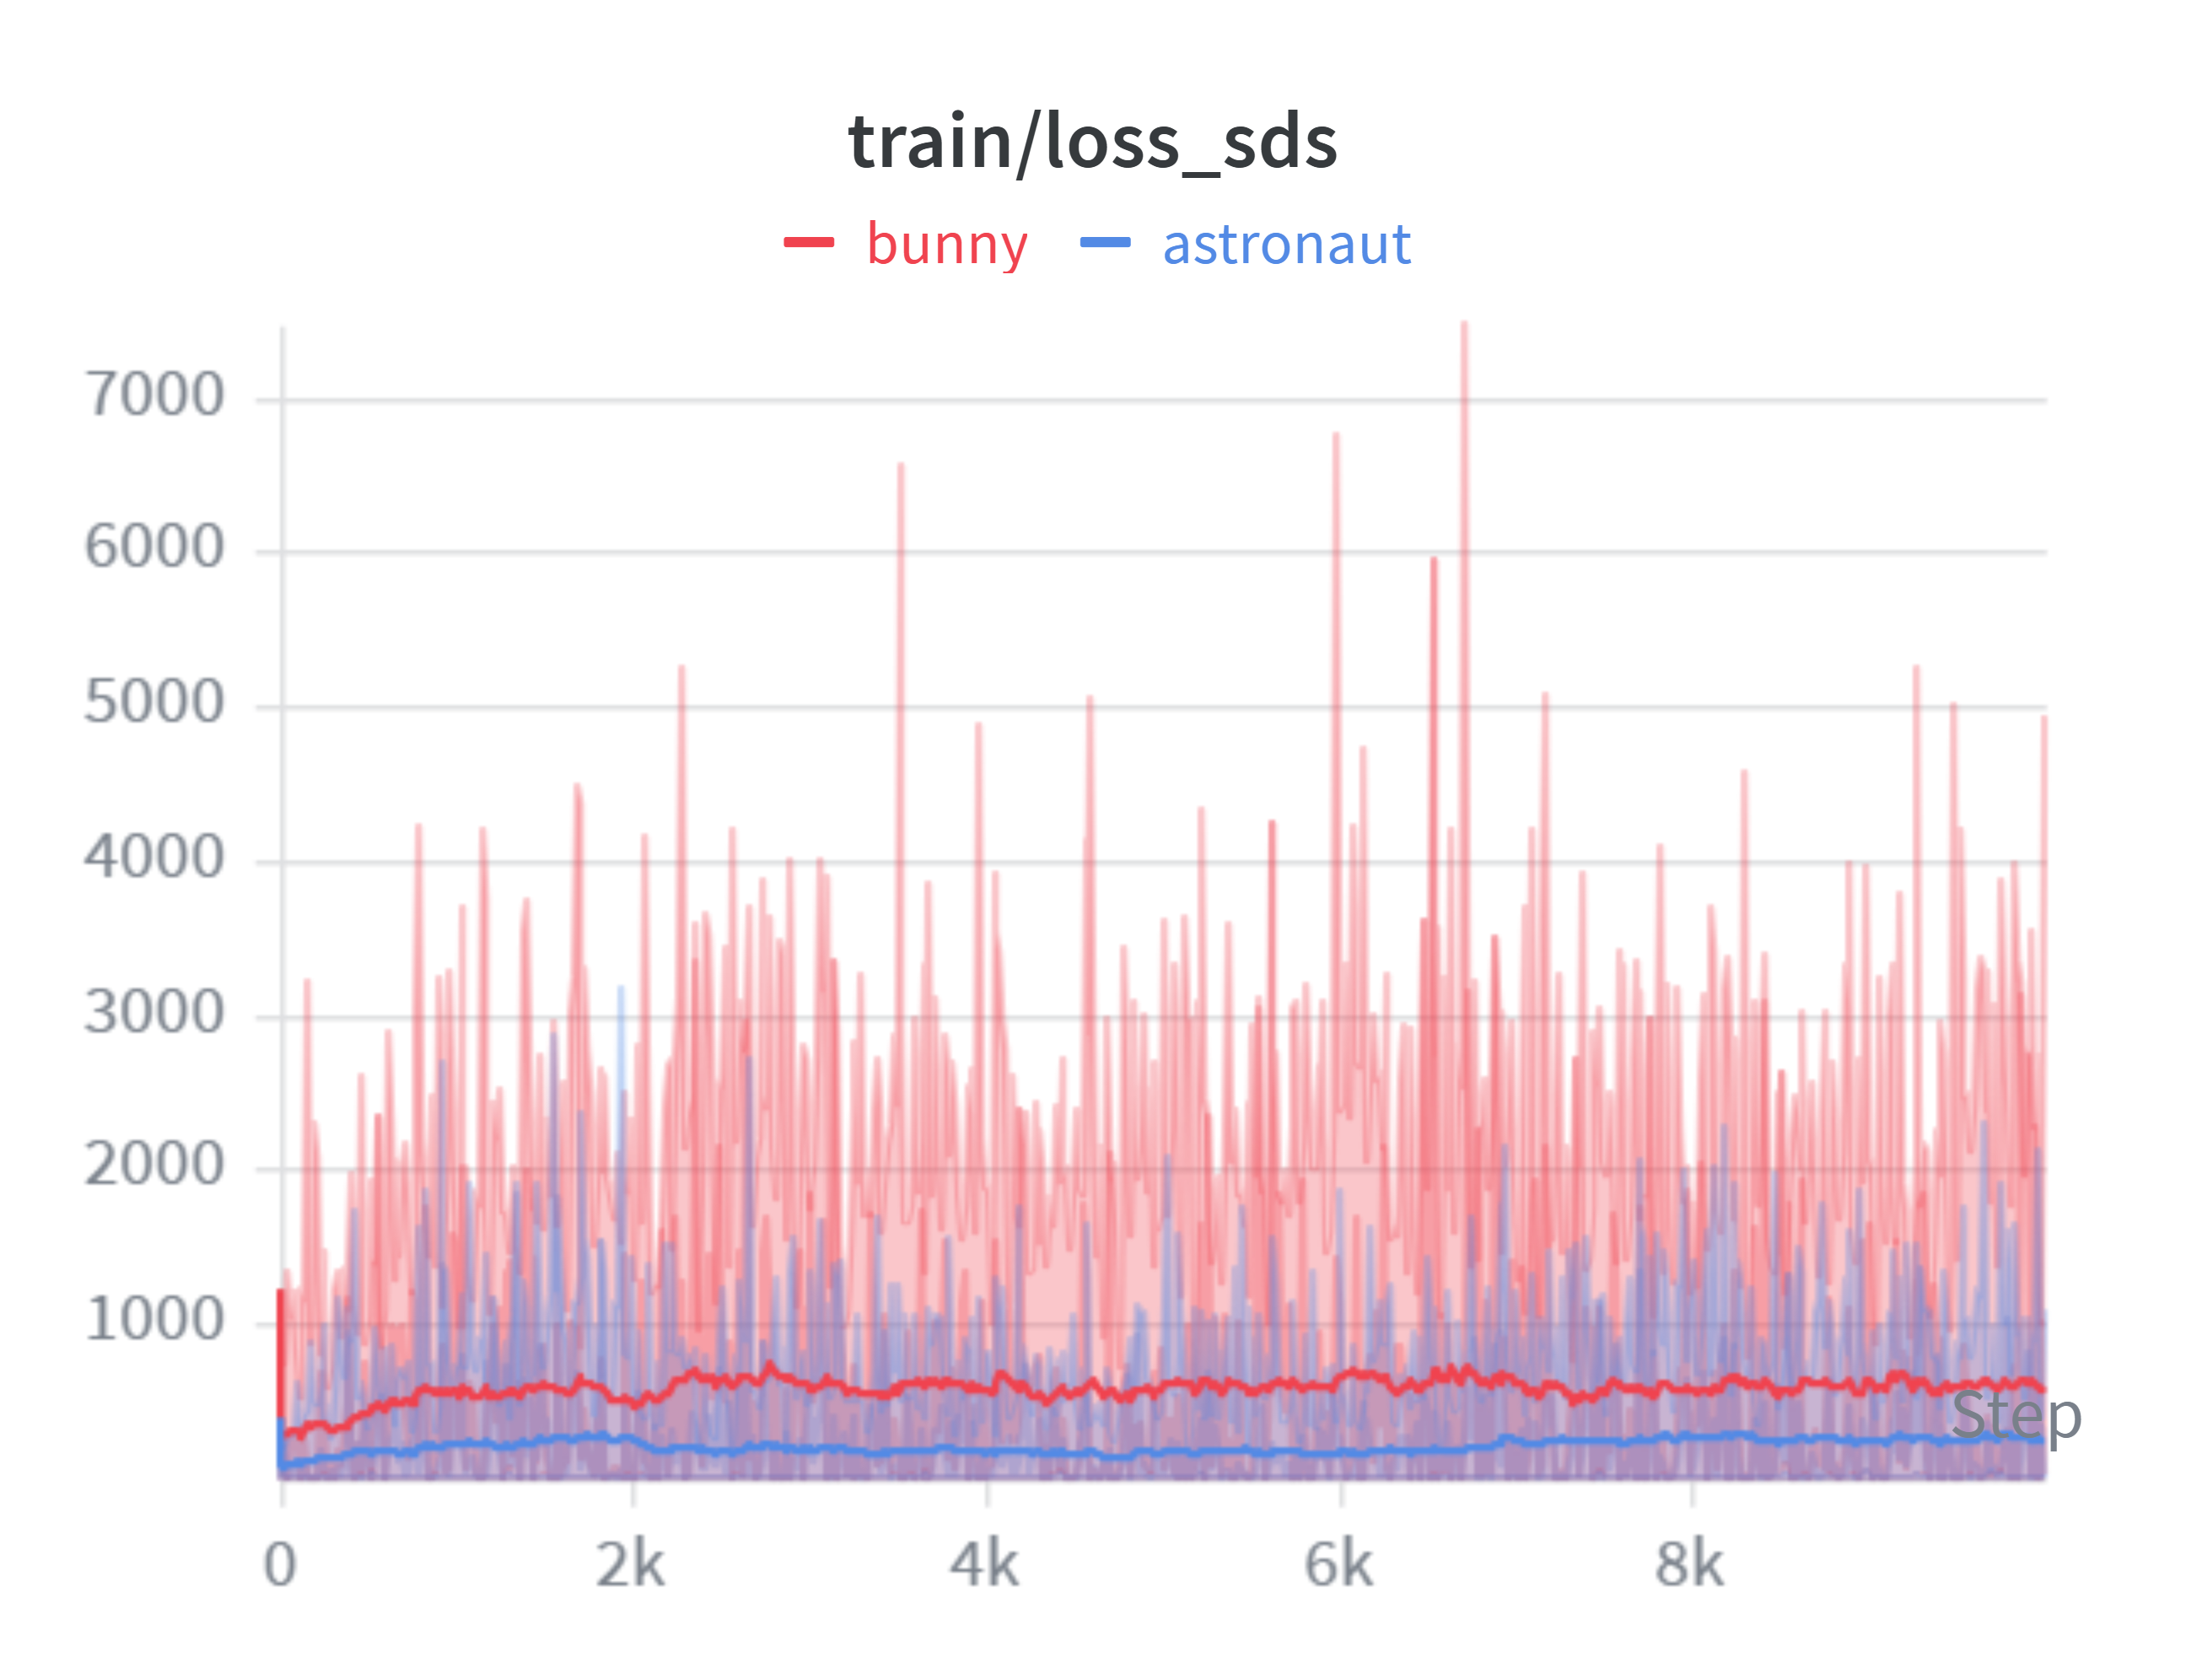
\includegraphics[width=\linewidth]{figures/task1/objectB/sds_loss.png}
		\caption{SDS Loss}
	\end{subfigure}
	\hfill
	\begin{subfigure}{0.4\textwidth}
		\centering
		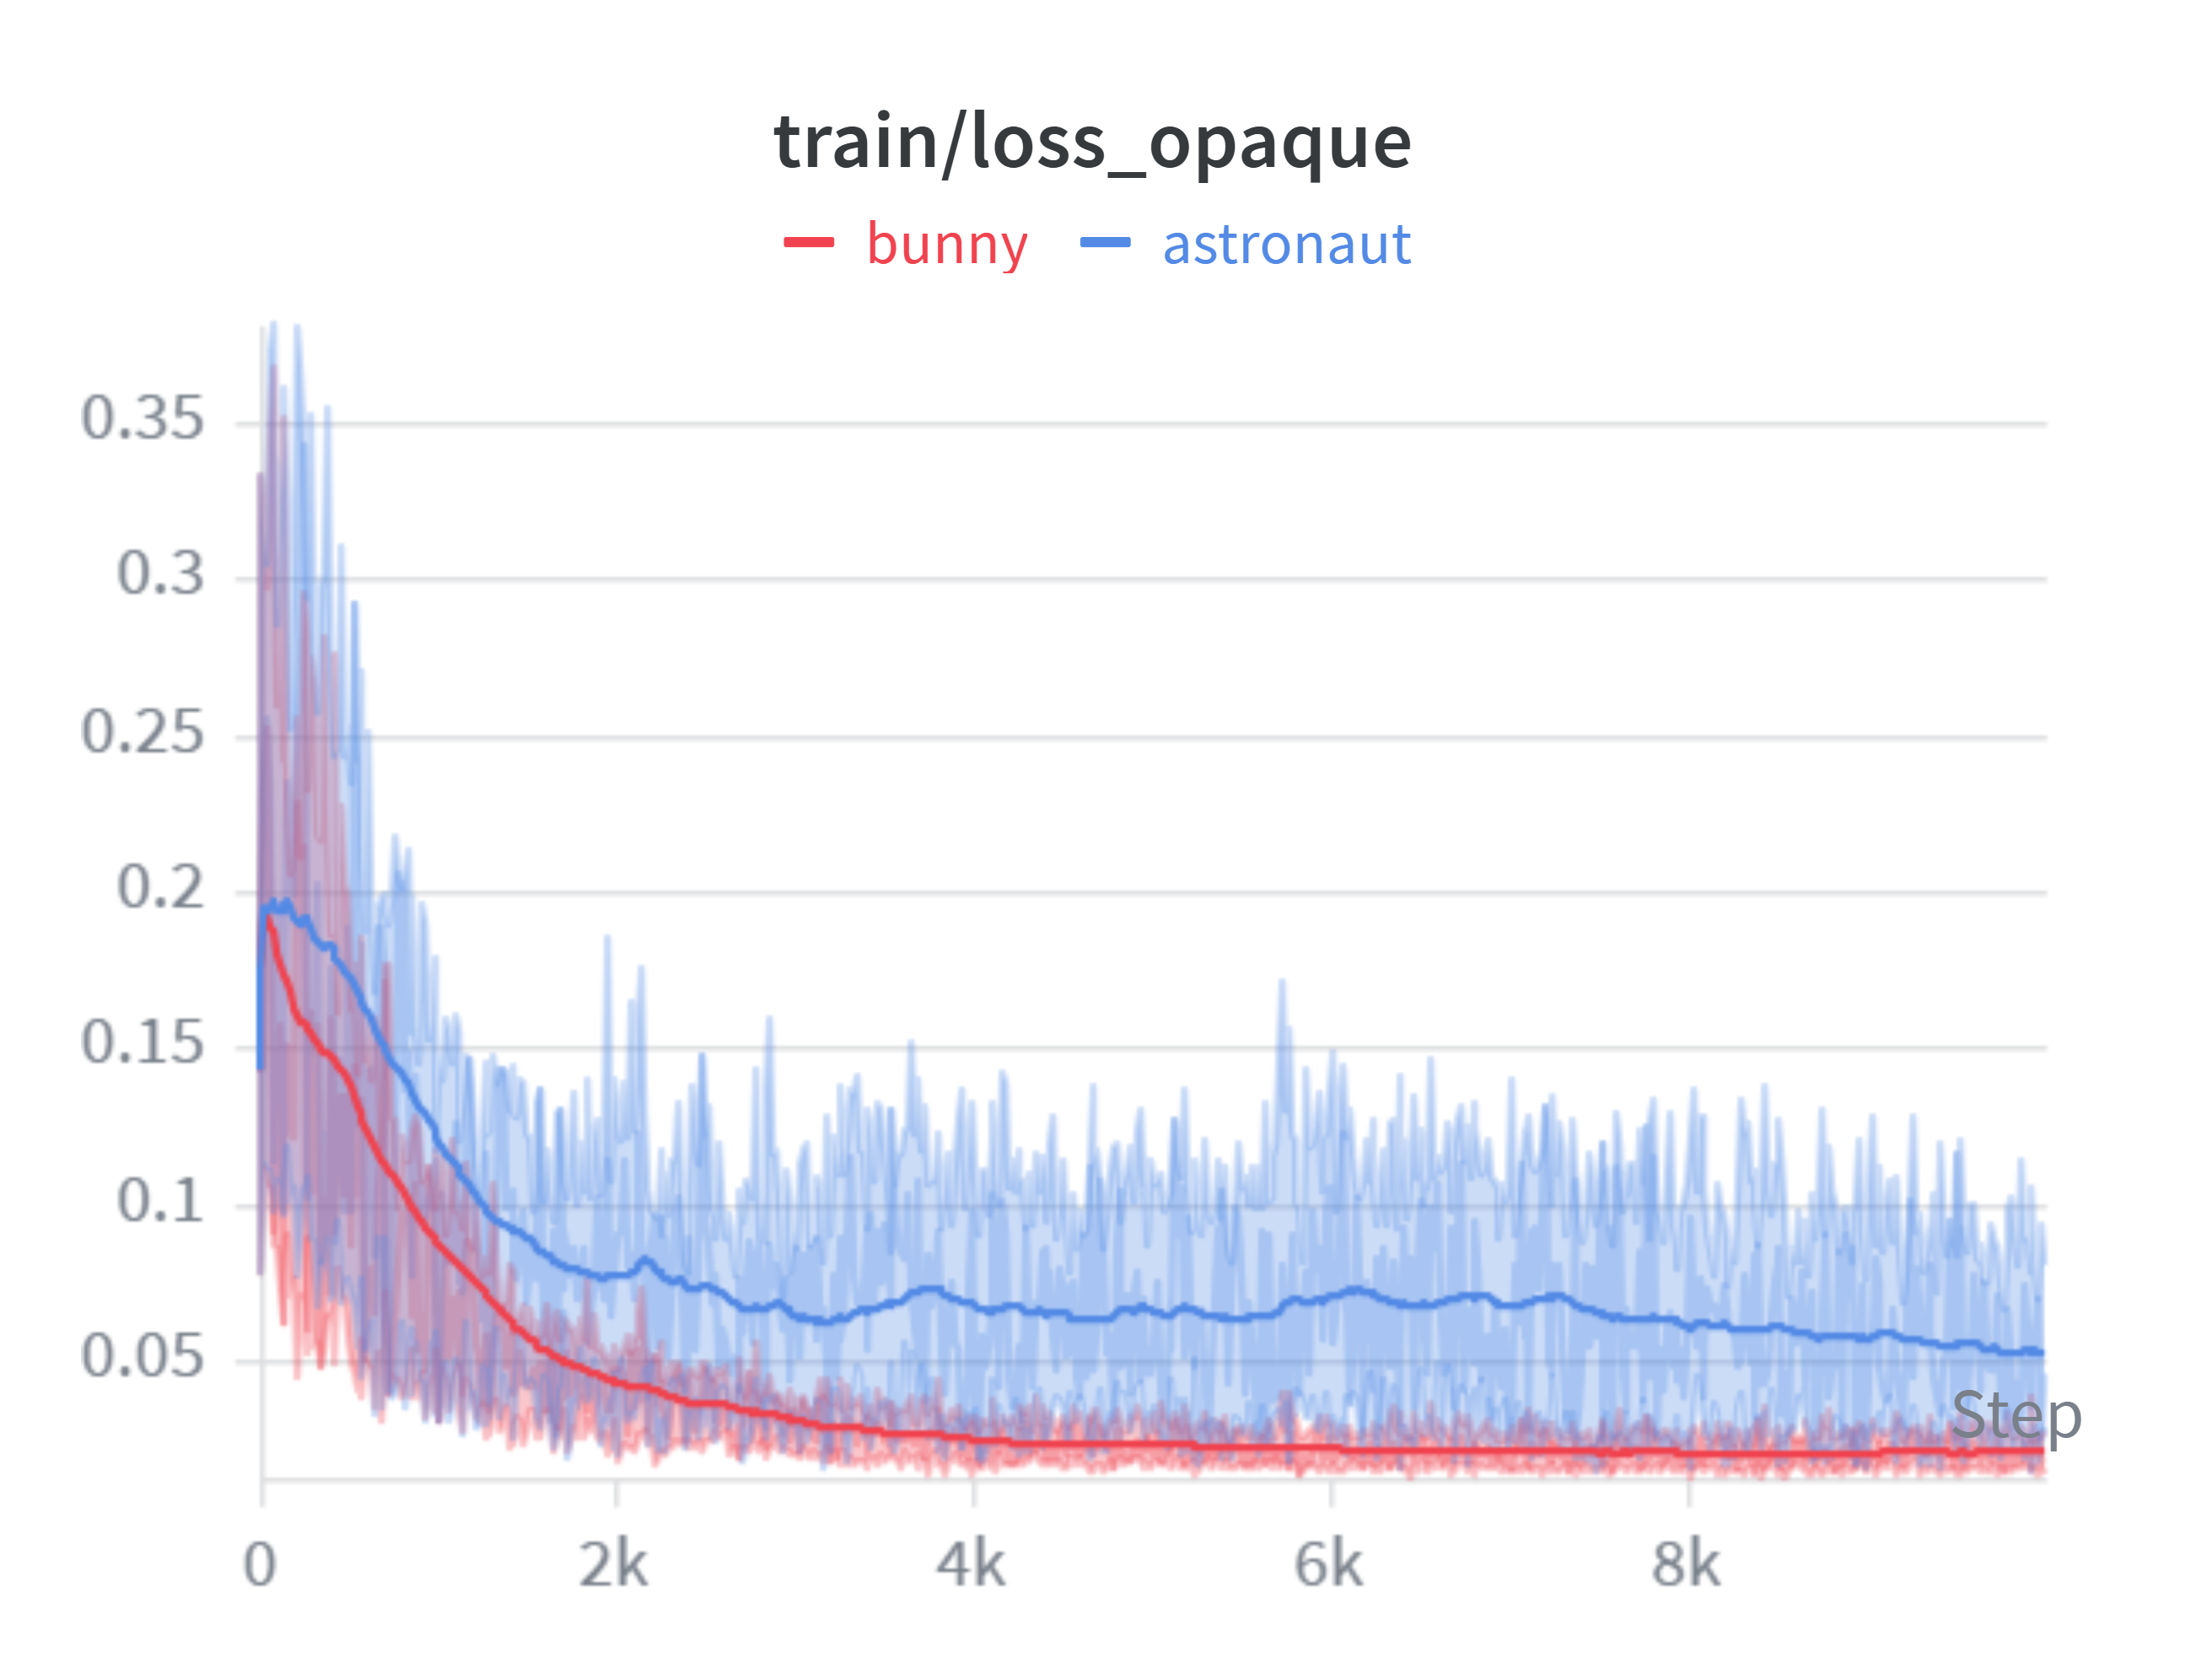
\includegraphics[width=\linewidth]{figures/task1/objectB/opaque_loss.png}
		\caption{Opaque Loss}
	\end{subfigure}
	
	\vspace{0.5cm} % 行间距，可以根据需要调整
	
	% 第二行
	\begin{subfigure}{0.4\textwidth}
		\centering
		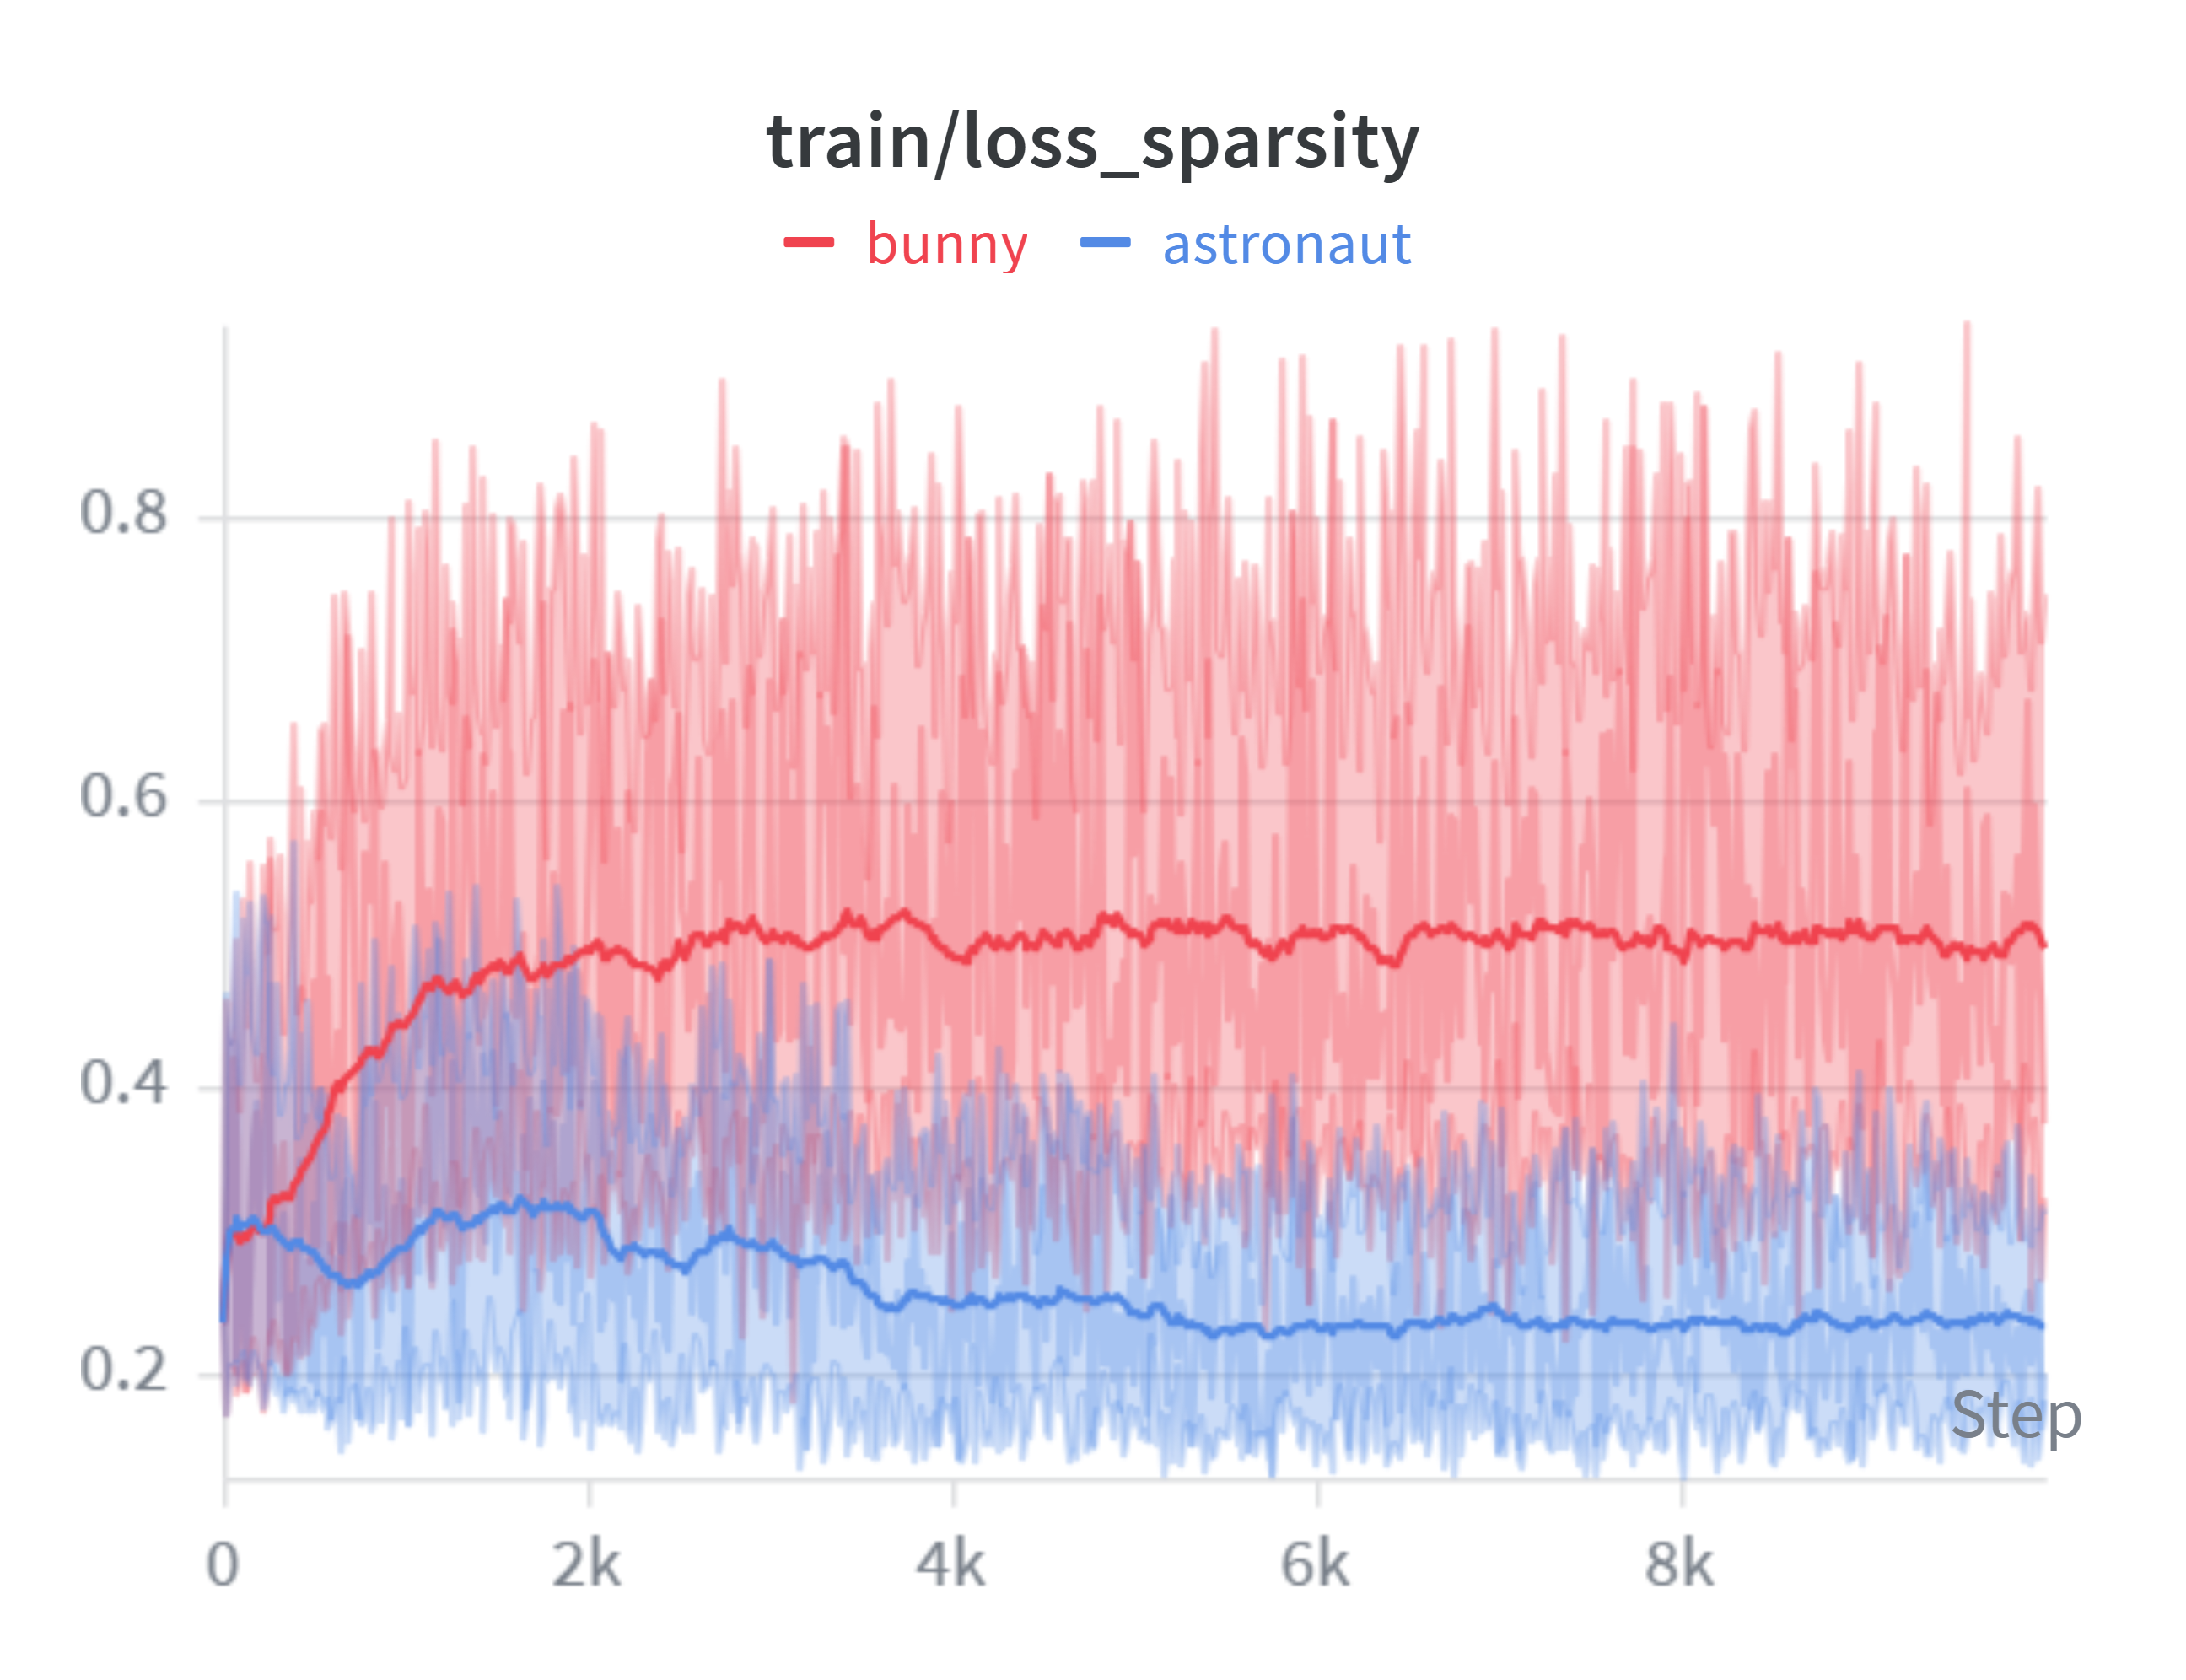
\includegraphics[width=\linewidth]{figures/task1/objectB/sparsity_loss.png}
		\caption{Sparsity Loss}
	\end{subfigure}
	\hfill
	\begin{subfigure}{0.4\textwidth}
		\centering
		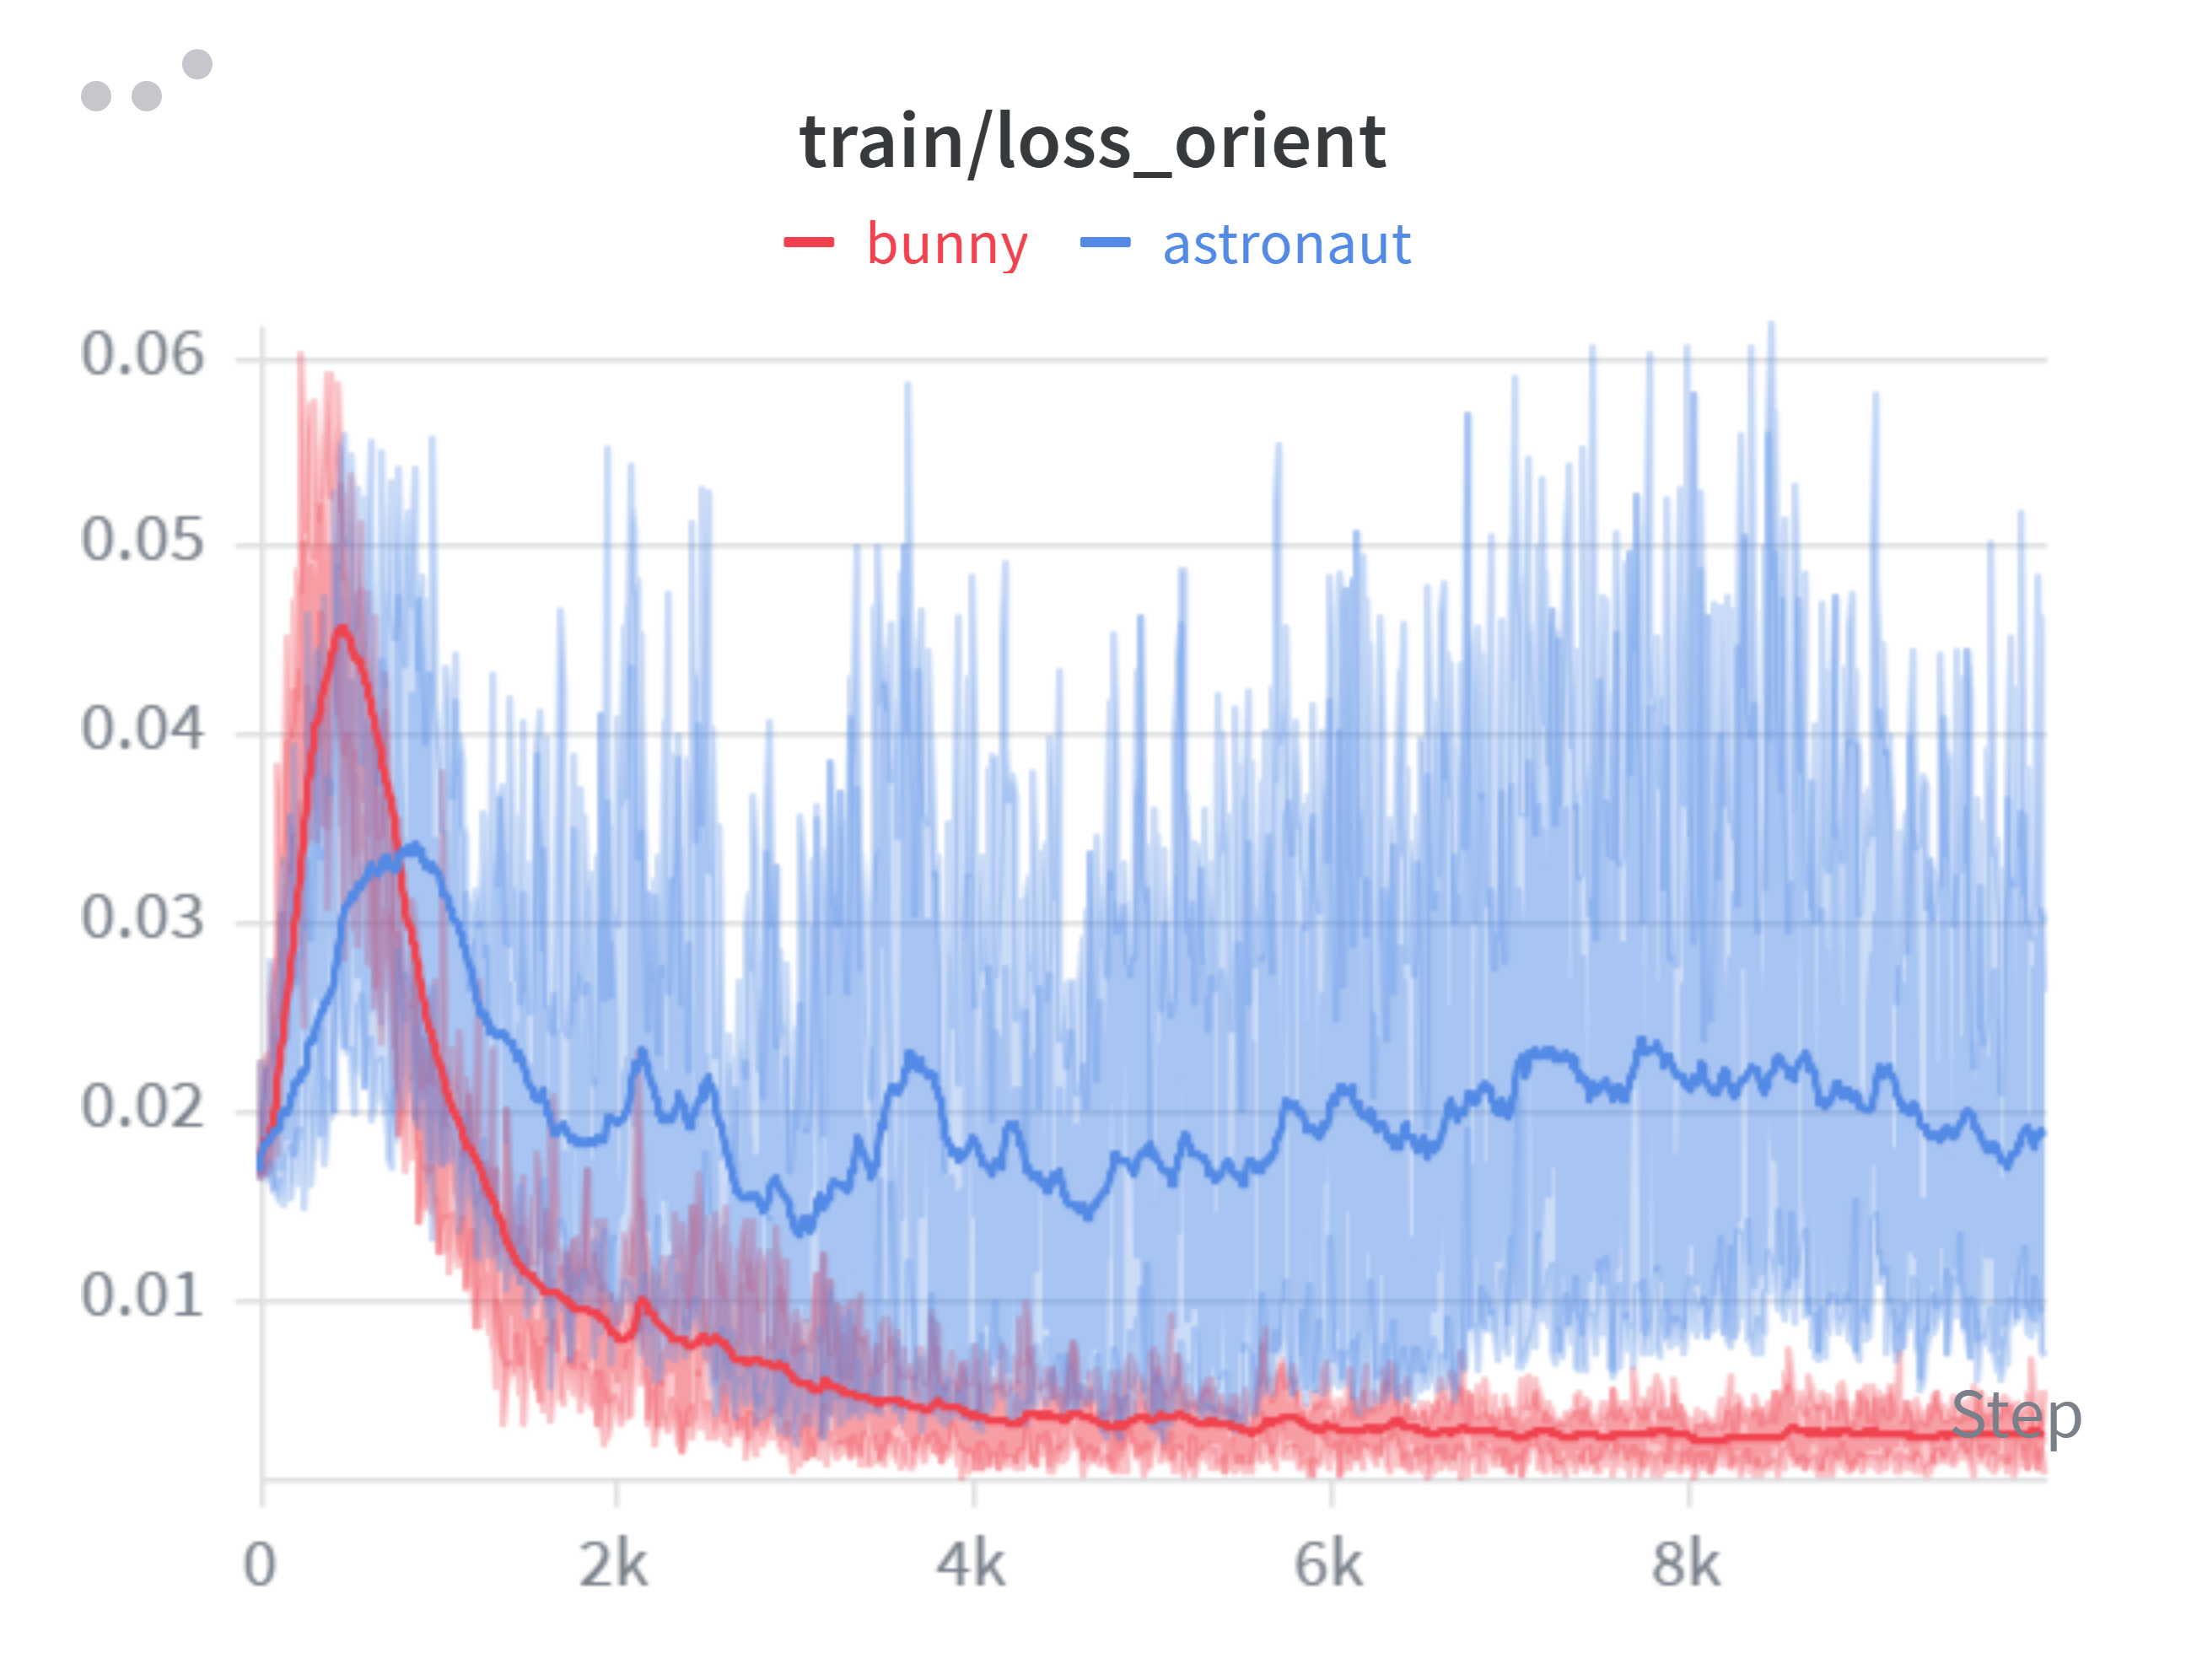
\includegraphics[width=\linewidth]{figures/task1/objectB/orient_loss.png}
		\caption{Orient Loss}
	\end{subfigure}
	
	\caption{Visualization results of generated 3D objects and training loss functions.}
	\label{fig:results_and_losses}
\end{figure}

We can see from the model visualizations that the astronaut has a relatively less smoother outfit and less appropriate color distribution, this may because that the pre-trained model doesn't have enough information compared with the bunny.

As for the training dynamics, here are our analysis:

SDS Loss exhibits extremely large magnitude values, reaching into the thousands, accompanied by very high variance and strong oscillations. Unlike typical supervised learning objectives, it does not demonstrate a smooth and monotonic decreasing trend during optimization. In 3D generative tasks, SDS Loss is derived from a pretrained diffusion model and fundamentally provides gradient directions in the parameter space rather than serving as an absolute scalar objective to be minimized to zero. Therefore, this behavior is ordinary. Comparing the two objects, the Bunny (red curve) shows significantly higher baseline values and variance than the Astronaut (blue curve), suggesting that the diffusion model provides more uncertain or higher-variance gradient guidance for the Bunny, possibly due to a more complex and unsmooth structure of the astronaut.

Opaque Loss decreases rapidly during the early stages of training and then gradually approaches a stable asymptotic plateau. This loss typically acts as a regularization term that removes floating artifacts and encourages the model to produce solid geometry. The Bunny converges very quickly and stabilizes near zero with minimal noise, whereas the Astronaut also decreases but eventually stabilizes at a relatively higher mean value (approximately 0.05 to 0.1) and retains noticeable variance in later stages. This indicates that the Astronaut presents a more challenging optimization landscape for opacity regularization.But the total structure is still clear.

Sparsity Loss increases rapidly in the early training stage before entering a highly oscillatory plateau. This reflects the constraint on spatial occupancy, encouraging empty space outside the object region. The initial increase indicates that the model is expanding its occupied volume while constructing the coarse geometry, while the subsequent plateau reflects a dynamic equilibrium between forming complete structures and maintaining spatial sparsity. The Bunny stabilizes at a relatively higher level (around 0.5), while the Astronaut stabilizes at a lower value (around 0.2). Suggesting that the Bunny occupies a more spatially extensive or volumetrically dense structure, resulting in higher sparsity penalties,which is aligned with the visualization results.

Orient Loss demonstrates a characteristic “spike-then-decay” behavior. This loss is typically used to regularize surface normals, ensuring smooth and physically consistent surface orientations while preventing jagged artifacts. The initial spike occurs when the model begins forming its coarse geometry and surface normals are highly disordered. As training progresses and the geometry becomes smoother, the loss decreases and converges. The Bunny reaches its peak around 1000 steps and then converges smoothly toward near-zero values, indicating highly optimized surface smoothness. In contrast, the Astronaut peaks slightly earlier but retains higher fluctuations and a non-negligible residual value (around 0.02), suggesting that its surface geometry is more complex.








\subsubsection{Object C}
In this section, the following picture is trained:

\begin{figure}[H]
	\centering
	
	% 第一张图（左边）
	\begin{subfigure}{0.4\textwidth}
		\centering
		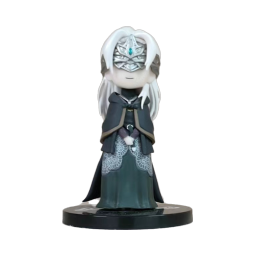
\includegraphics[width=\linewidth]{figures/task1/objectC/firekeeper_rgba.png} % 第一张图片路径
		\caption{Firekeeper(threestudio)}
	\end{subfigure}
	\hfill % 两张图之间的间距
	% 第二张图（右边）
	\begin{subfigure}{0.4\textwidth}
		\centering
		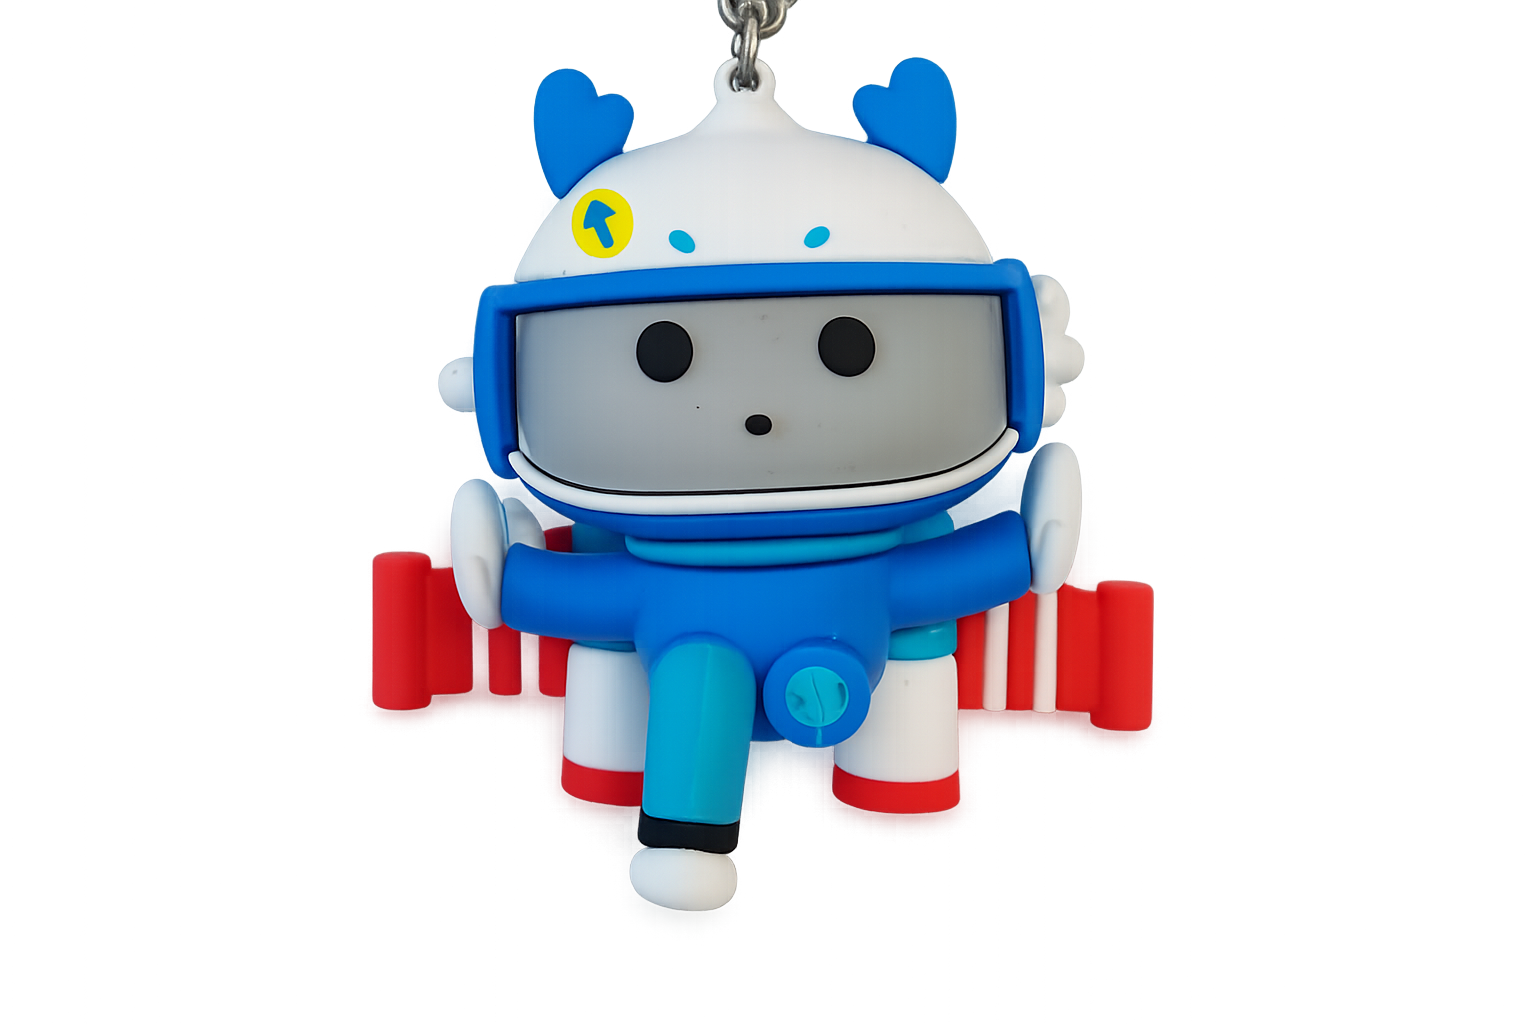
\includegraphics[width=\linewidth]{figures/task1/objectC/cute_robot_rgba.png} % 替换为你的第二张图片路径
		\caption{Cute Astronaut Robot(Ours)}
	\end{subfigure}

\end{figure}


Each training takes about \textbf{30min}(coarse)+\textbf{30min}(refine), the rendering results and training dynamics are as follow:

\begin{figure}[H]
	\centering
	
	%================ 第一组：Astronaut =================
	\begin{subfigure}{0.25\textwidth}
		\centering
		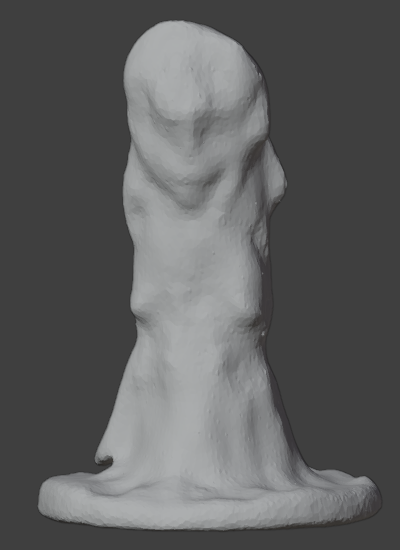
\includegraphics[width=\linewidth]{figures/task1/objectC/firekeeper_mesh.png}
		\caption{Firekeeper Mesh}
	\end{subfigure}
	\hfill
	\begin{subfigure}{0.25\textwidth}
		\centering
		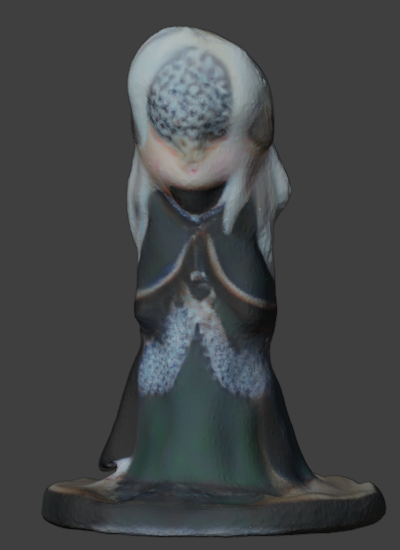
\includegraphics[width=\linewidth]{figures/task1/objectC/firekeeper_color.png}
		\caption{Firekeeper Color}
	\end{subfigure}
	\hfill
	\begin{subfigure}{0.25\textwidth}
		\centering
		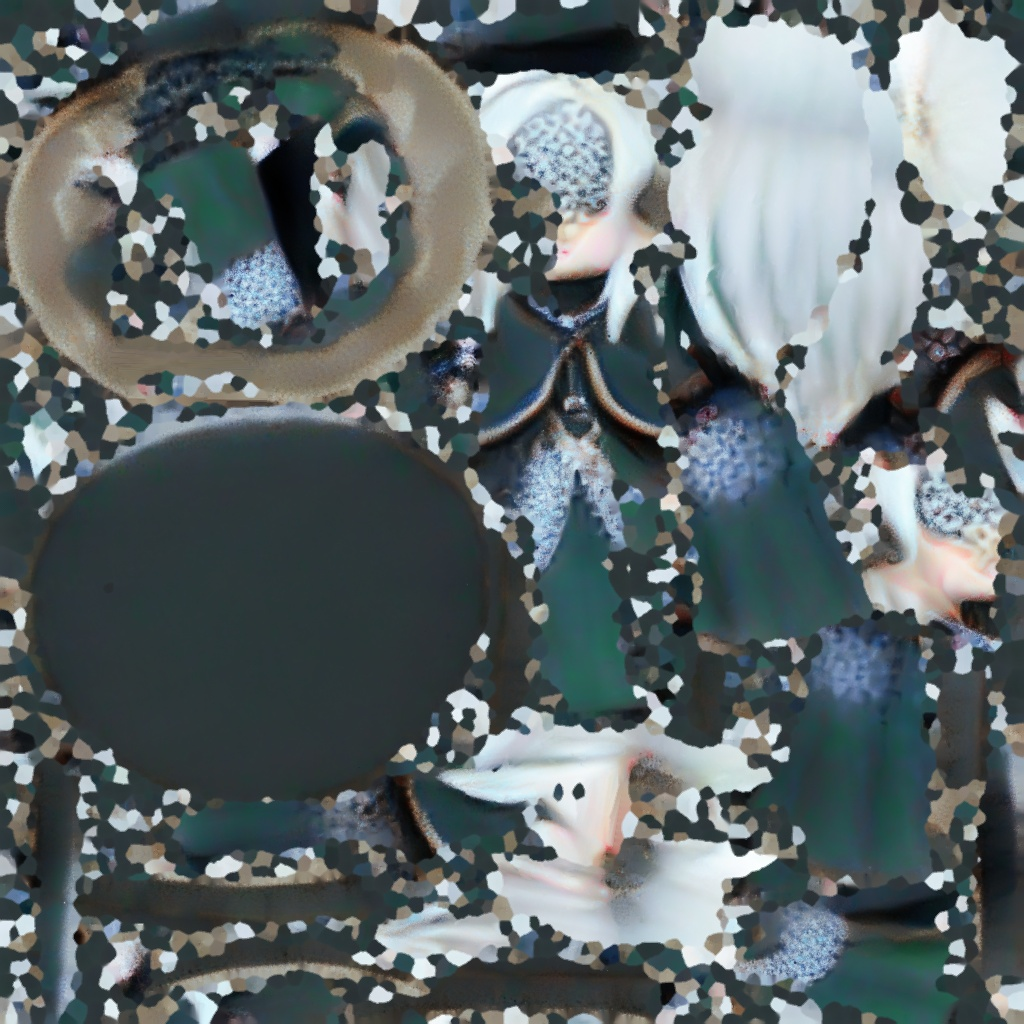
\includegraphics[width=\linewidth]{figures/task1/objectC/firekeeper_texture_kd.jpg}
		\caption{Firekeeper Texture}
	\end{subfigure}
	
	
\end{figure}




\begin{figure}[H]
	\centering
	
	% 第一张
	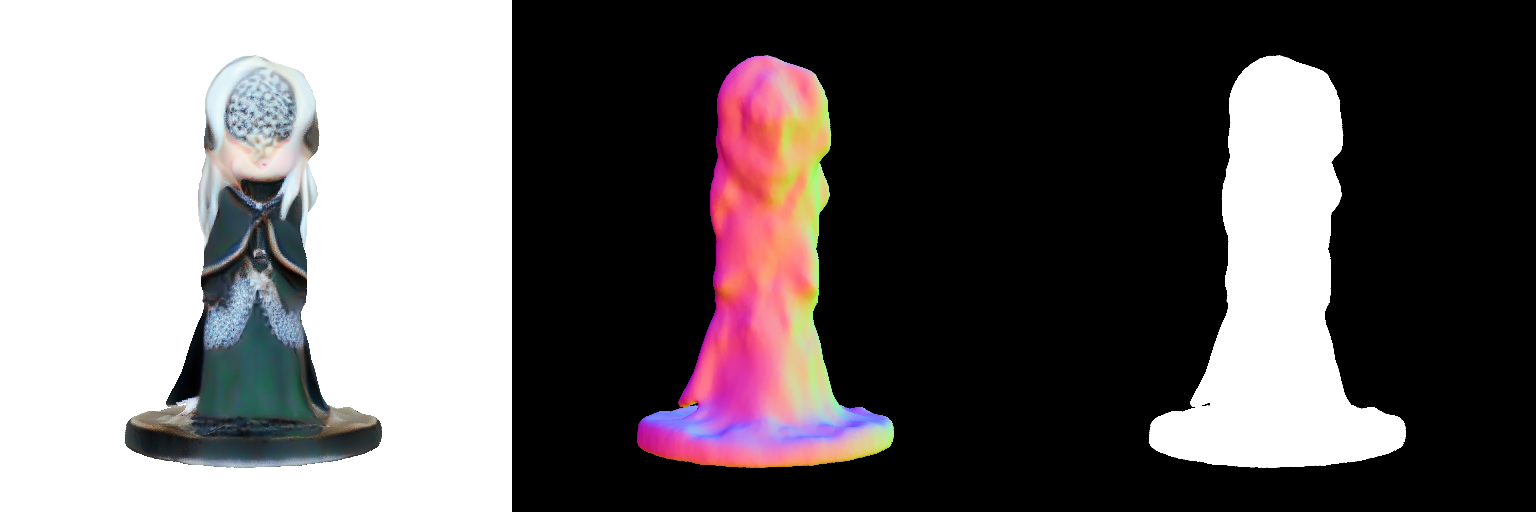
\includegraphics[width=0.6\textwidth]{figures/task1/objectC/firekeeper1.png} % 替换为你的实际路径

	
	\vspace{0.3cm} % 调整图片之间的垂直间距
	
	% 第二张
	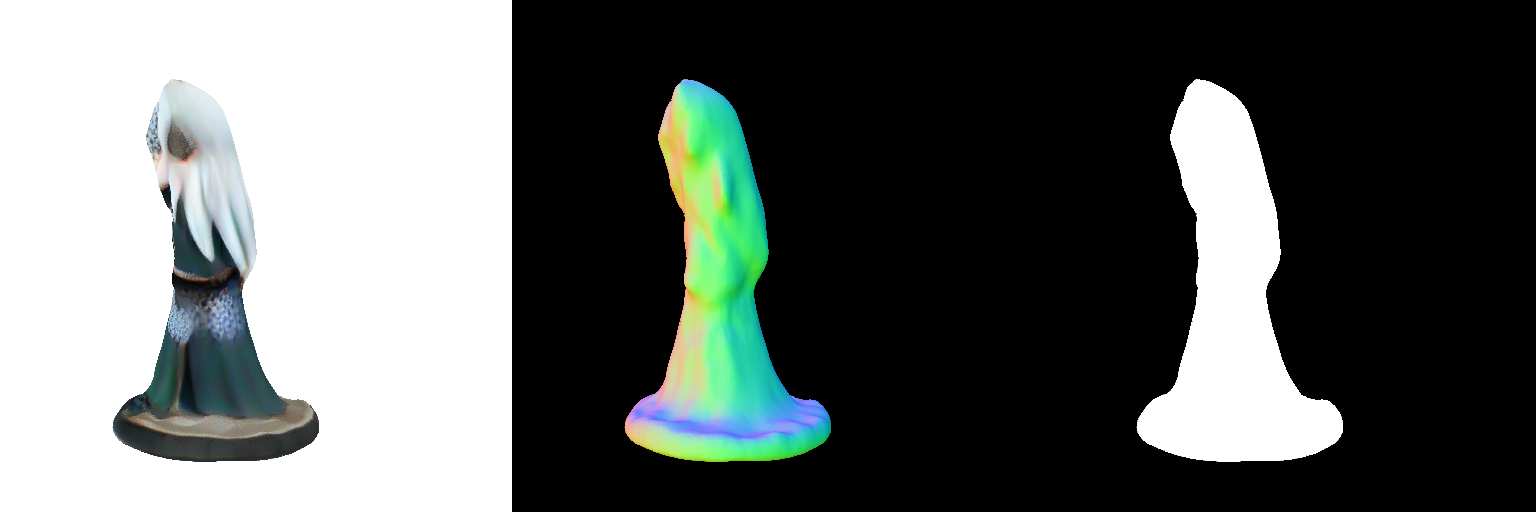
\includegraphics[width=0.6\textwidth]{figures/task1/objectC/firekeeper2.png}

	
	\vspace{0.3cm}
	
	% 第三张
	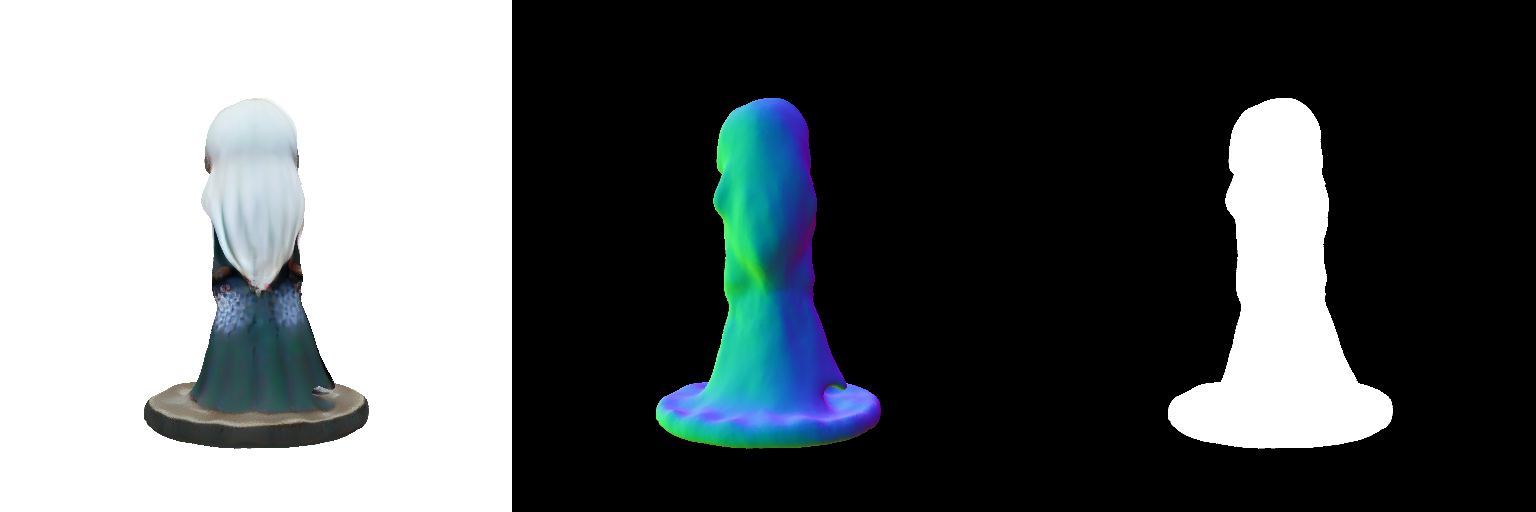
\includegraphics[width=0.6\textwidth]{figures/task1/objectC/firekeeper3.png}

	
	\vspace{0.3cm}
	
	% 第四张
	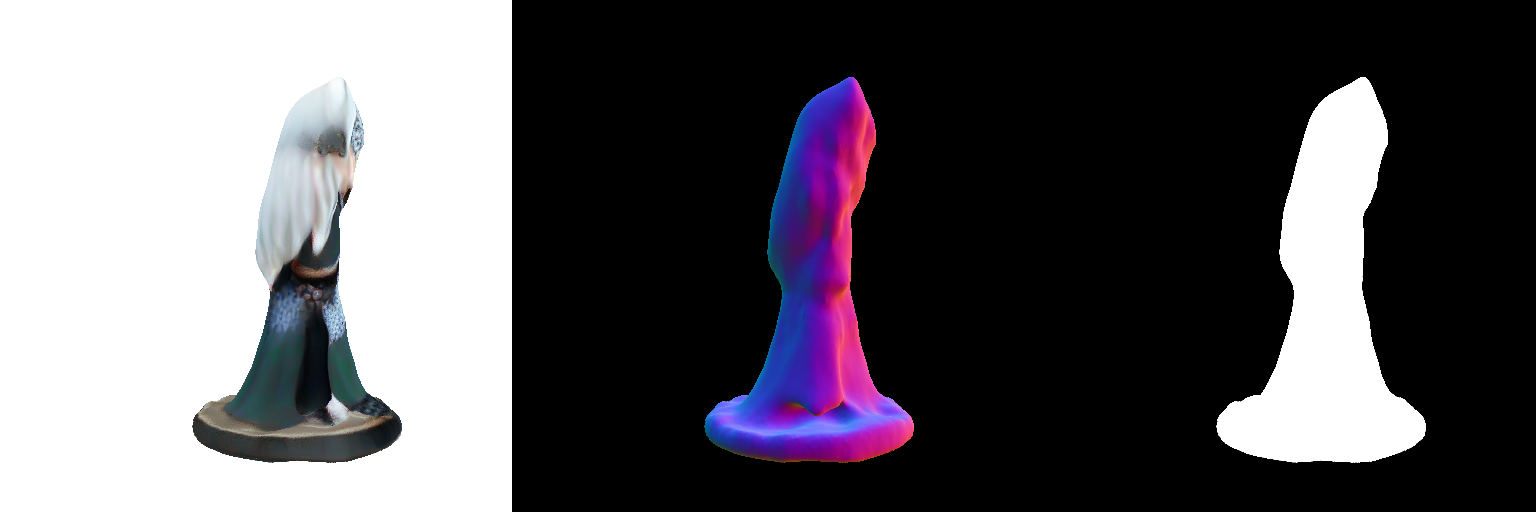
\includegraphics[width=0.6\textwidth]{figures/task1/objectC/firekeeper4.png}

	
	\caption{Different Viewpoints}
	\label{fig:firekeeper_vertical}
\end{figure}

\begin{figure}[H]
		\begin{subfigure}{0.25\textwidth}
		\centering
		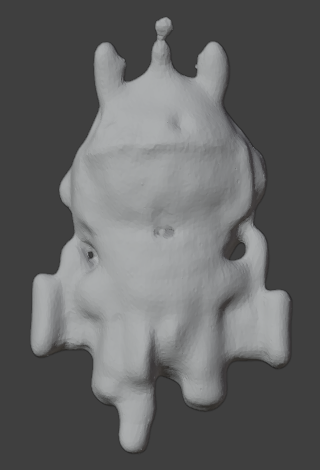
\includegraphics[width=\linewidth]{figures/task1/objectC/cute_robot_mesh.png}
		\caption{Robot Mesh}
	\end{subfigure}
	\hfill
	\begin{subfigure}{0.25\textwidth}
		\centering
		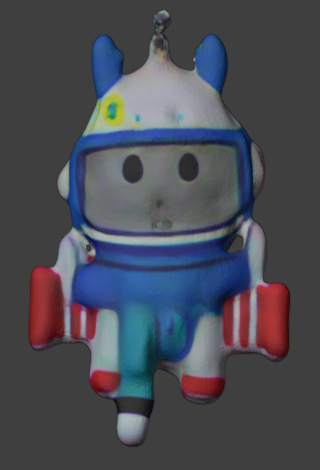
\includegraphics[width=\linewidth]{figures/task1/objectC/cute_robot_color.png}
		\caption{Robot Color}
	\end{subfigure}
	\hfill
	\begin{subfigure}{0.25\textwidth}
		\centering
		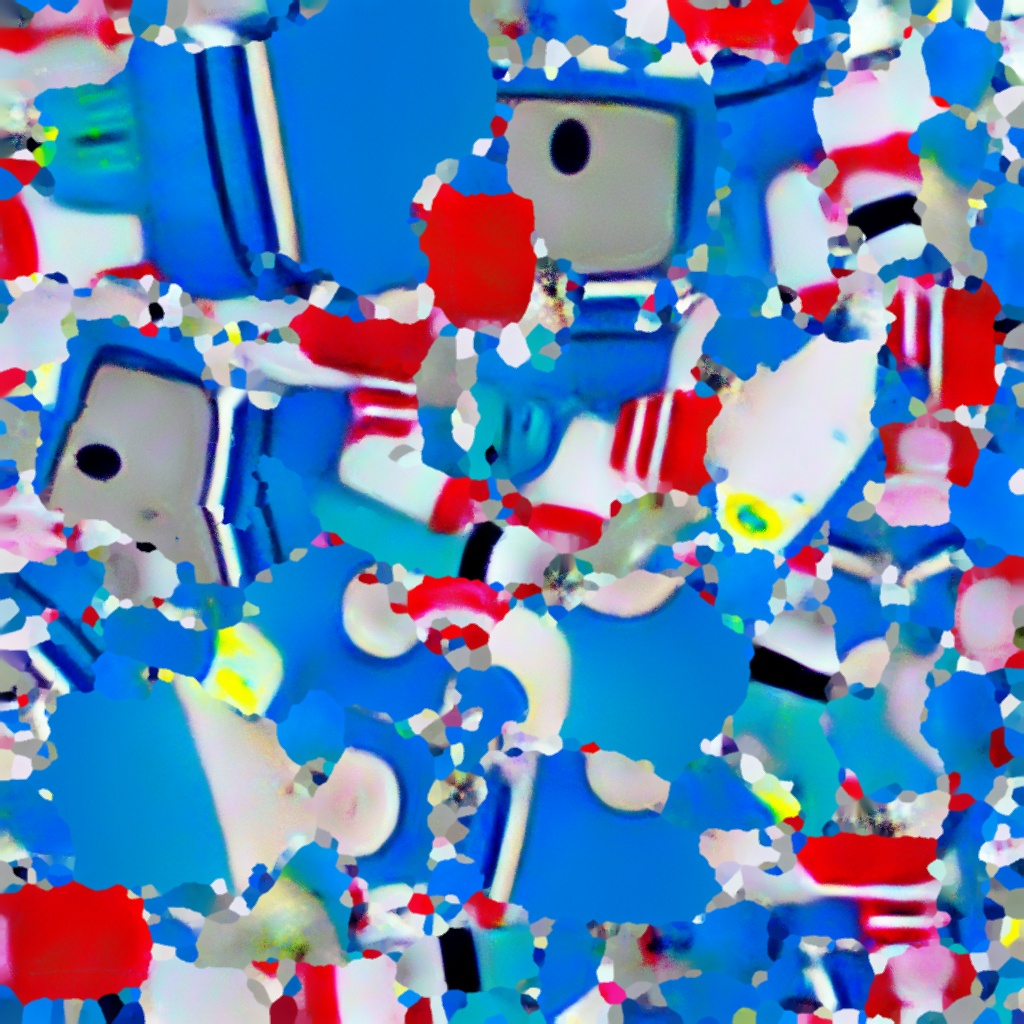
\includegraphics[width=\linewidth]{figures/task1/objectC/robot_texture_kd.jpg}
		\caption{Robot Texture}
	\end{subfigure}
\end{figure}

\begin{figure}[H]
	\centering
	
	% 第一张
	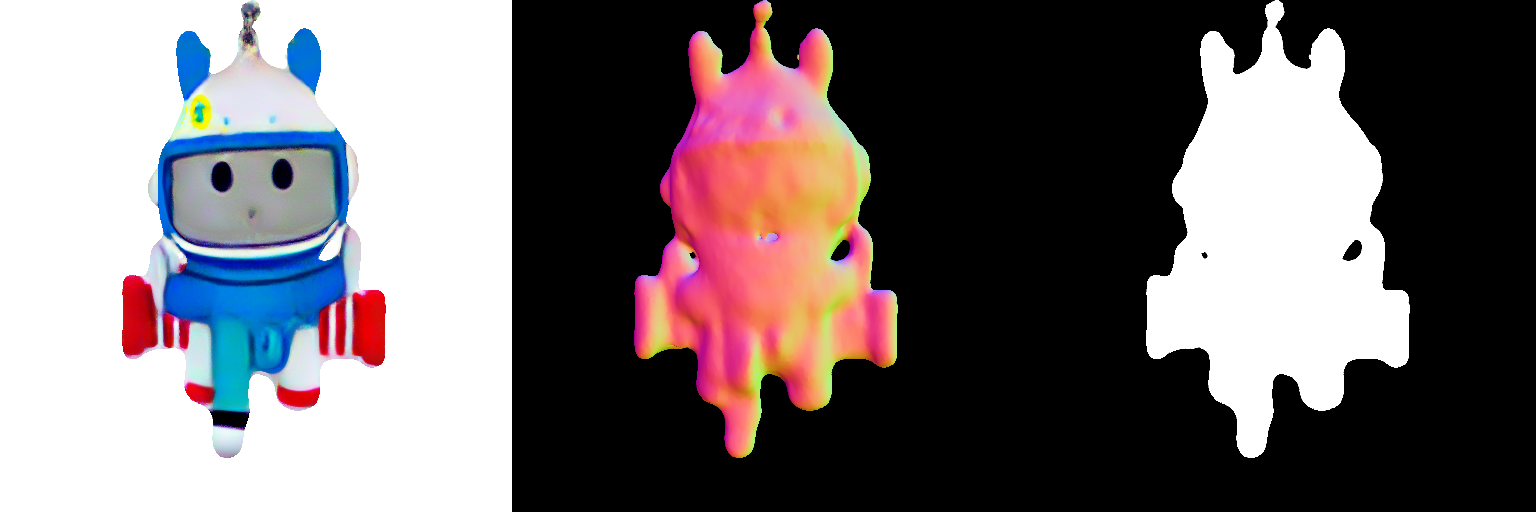
\includegraphics[width=0.6\textwidth]{figures/task1/objectC/robot1.png} % 替换为你的实际路径
	
	
	\vspace{0.3cm} % 调整图片之间的垂直间距
	
	% 第二张
	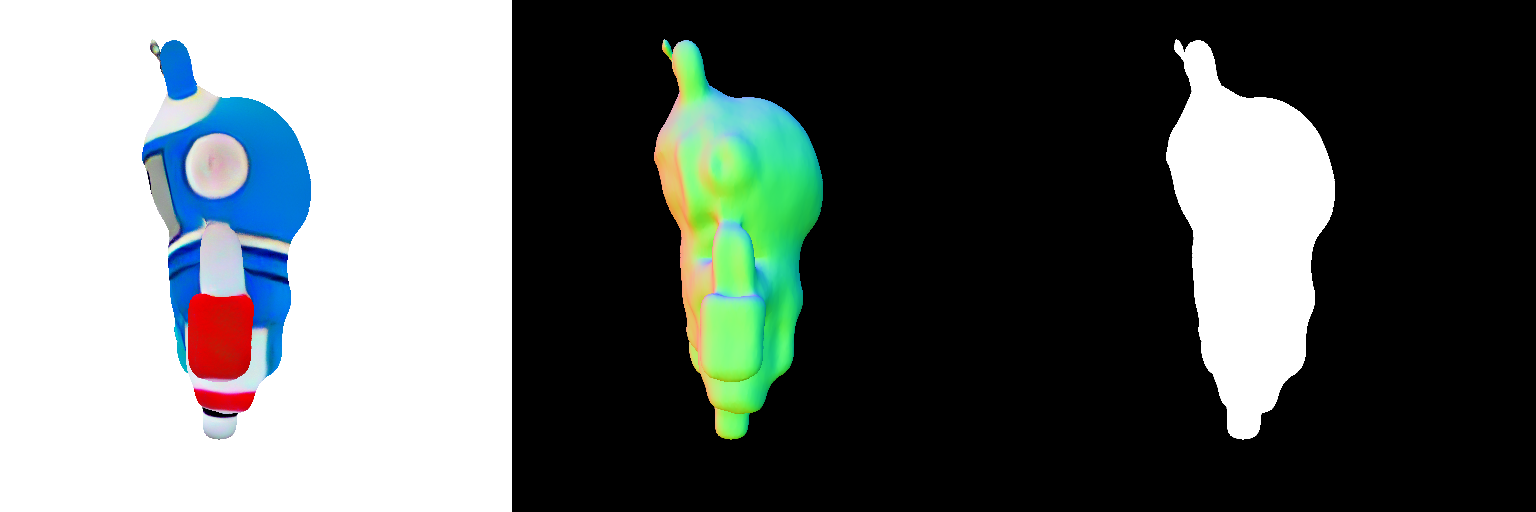
\includegraphics[width=0.6\textwidth]{figures/task1/objectC/robot2.png}
	
	
	\vspace{0.3cm}
	
	% 第三张
	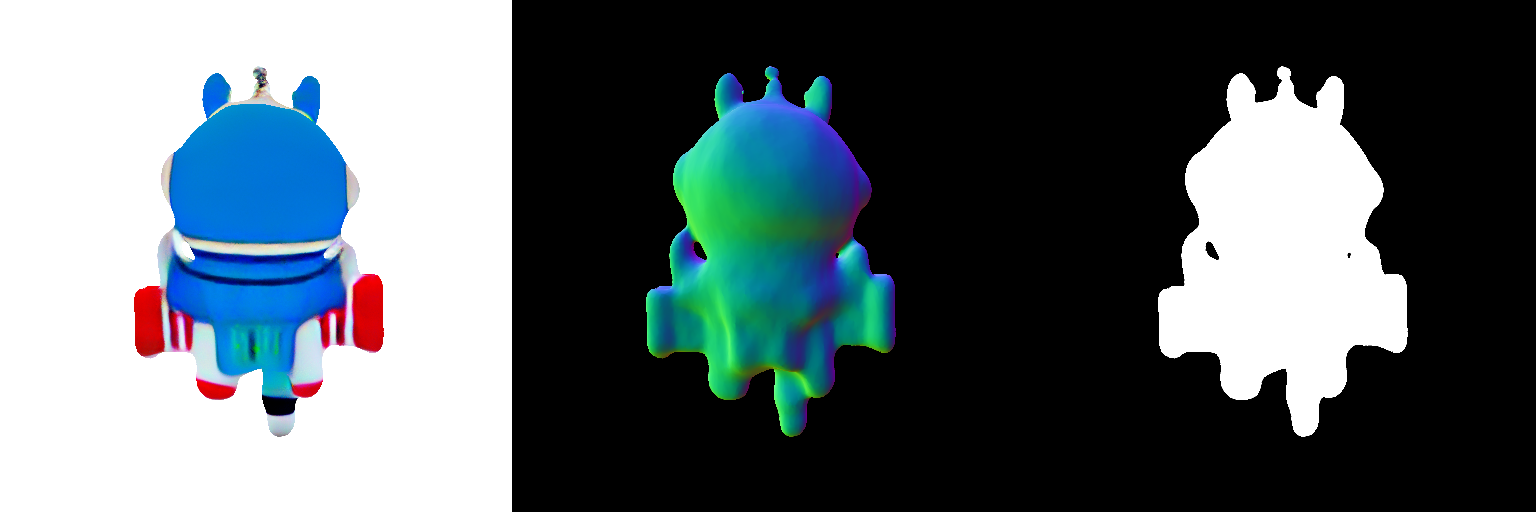
\includegraphics[width=0.6\textwidth]{figures/task1/objectC/robot3.png}
	
	
	\vspace{0.3cm}
	
	% 第四张
	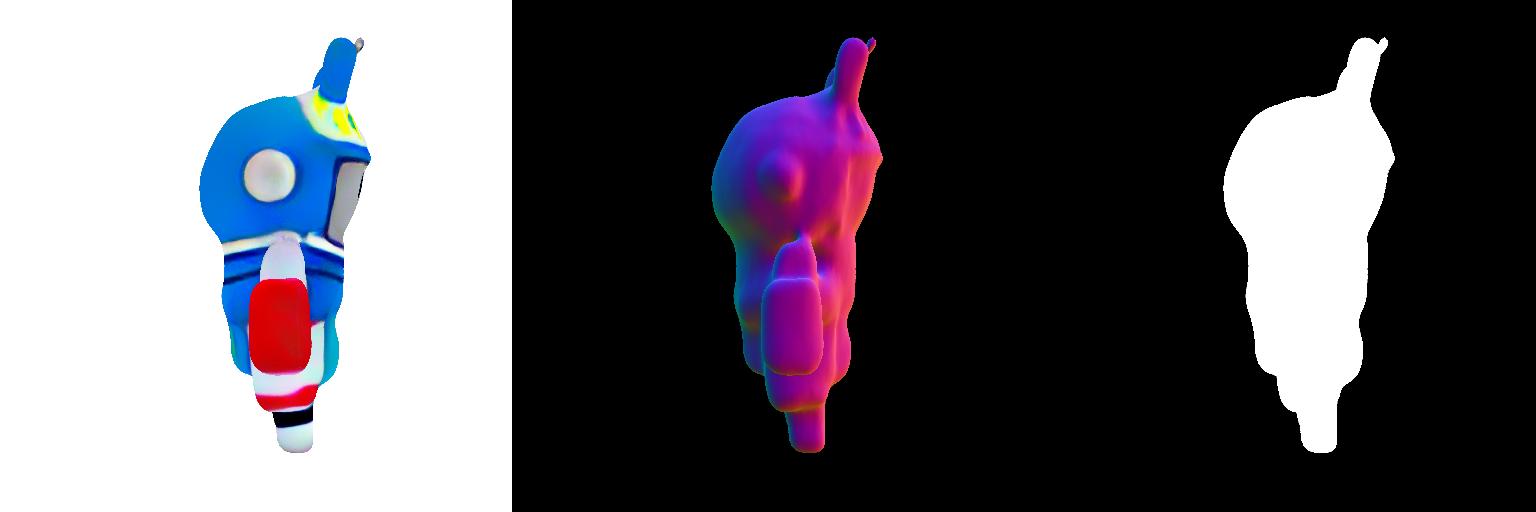
\includegraphics[width=0.6\textwidth]{figures/task1/objectC/robot4.png}
	
	
	\caption{Different Viewpoints}
	\label{fig:Robot_vertical}
\end{figure}



\begin{figure}[H]
	\centering
	
	% 第一张图（左边）
	\begin{subfigure}{0.48\textwidth}
		\centering
		
\includegraphics[width=\linewidth]{figures/task1/objectC/opaque_loss.png} % 第一张图片路径
		\caption{Firekeeper(threestudio)}
	\end{subfigure}
	\hfill % 两张图之间的间距
	% 第二张图（右边）
	\begin{subfigure}{0.48\textwidth}
		\centering
		
\includegraphics[width=\linewidth]{figures/task1/objectC/sparsity_loss.png} % 替换为你的第二张图片路径
		\caption{Cute Astronaut Robot(Ours)}
	\end{subfigure}
	
\end{figure}


\begin{figure*}[H]
	\centering
	
	%==================== 第一组：SDS Loss ====================
	\begin{subfigure}[t]{0.32\textwidth}
		\centering
		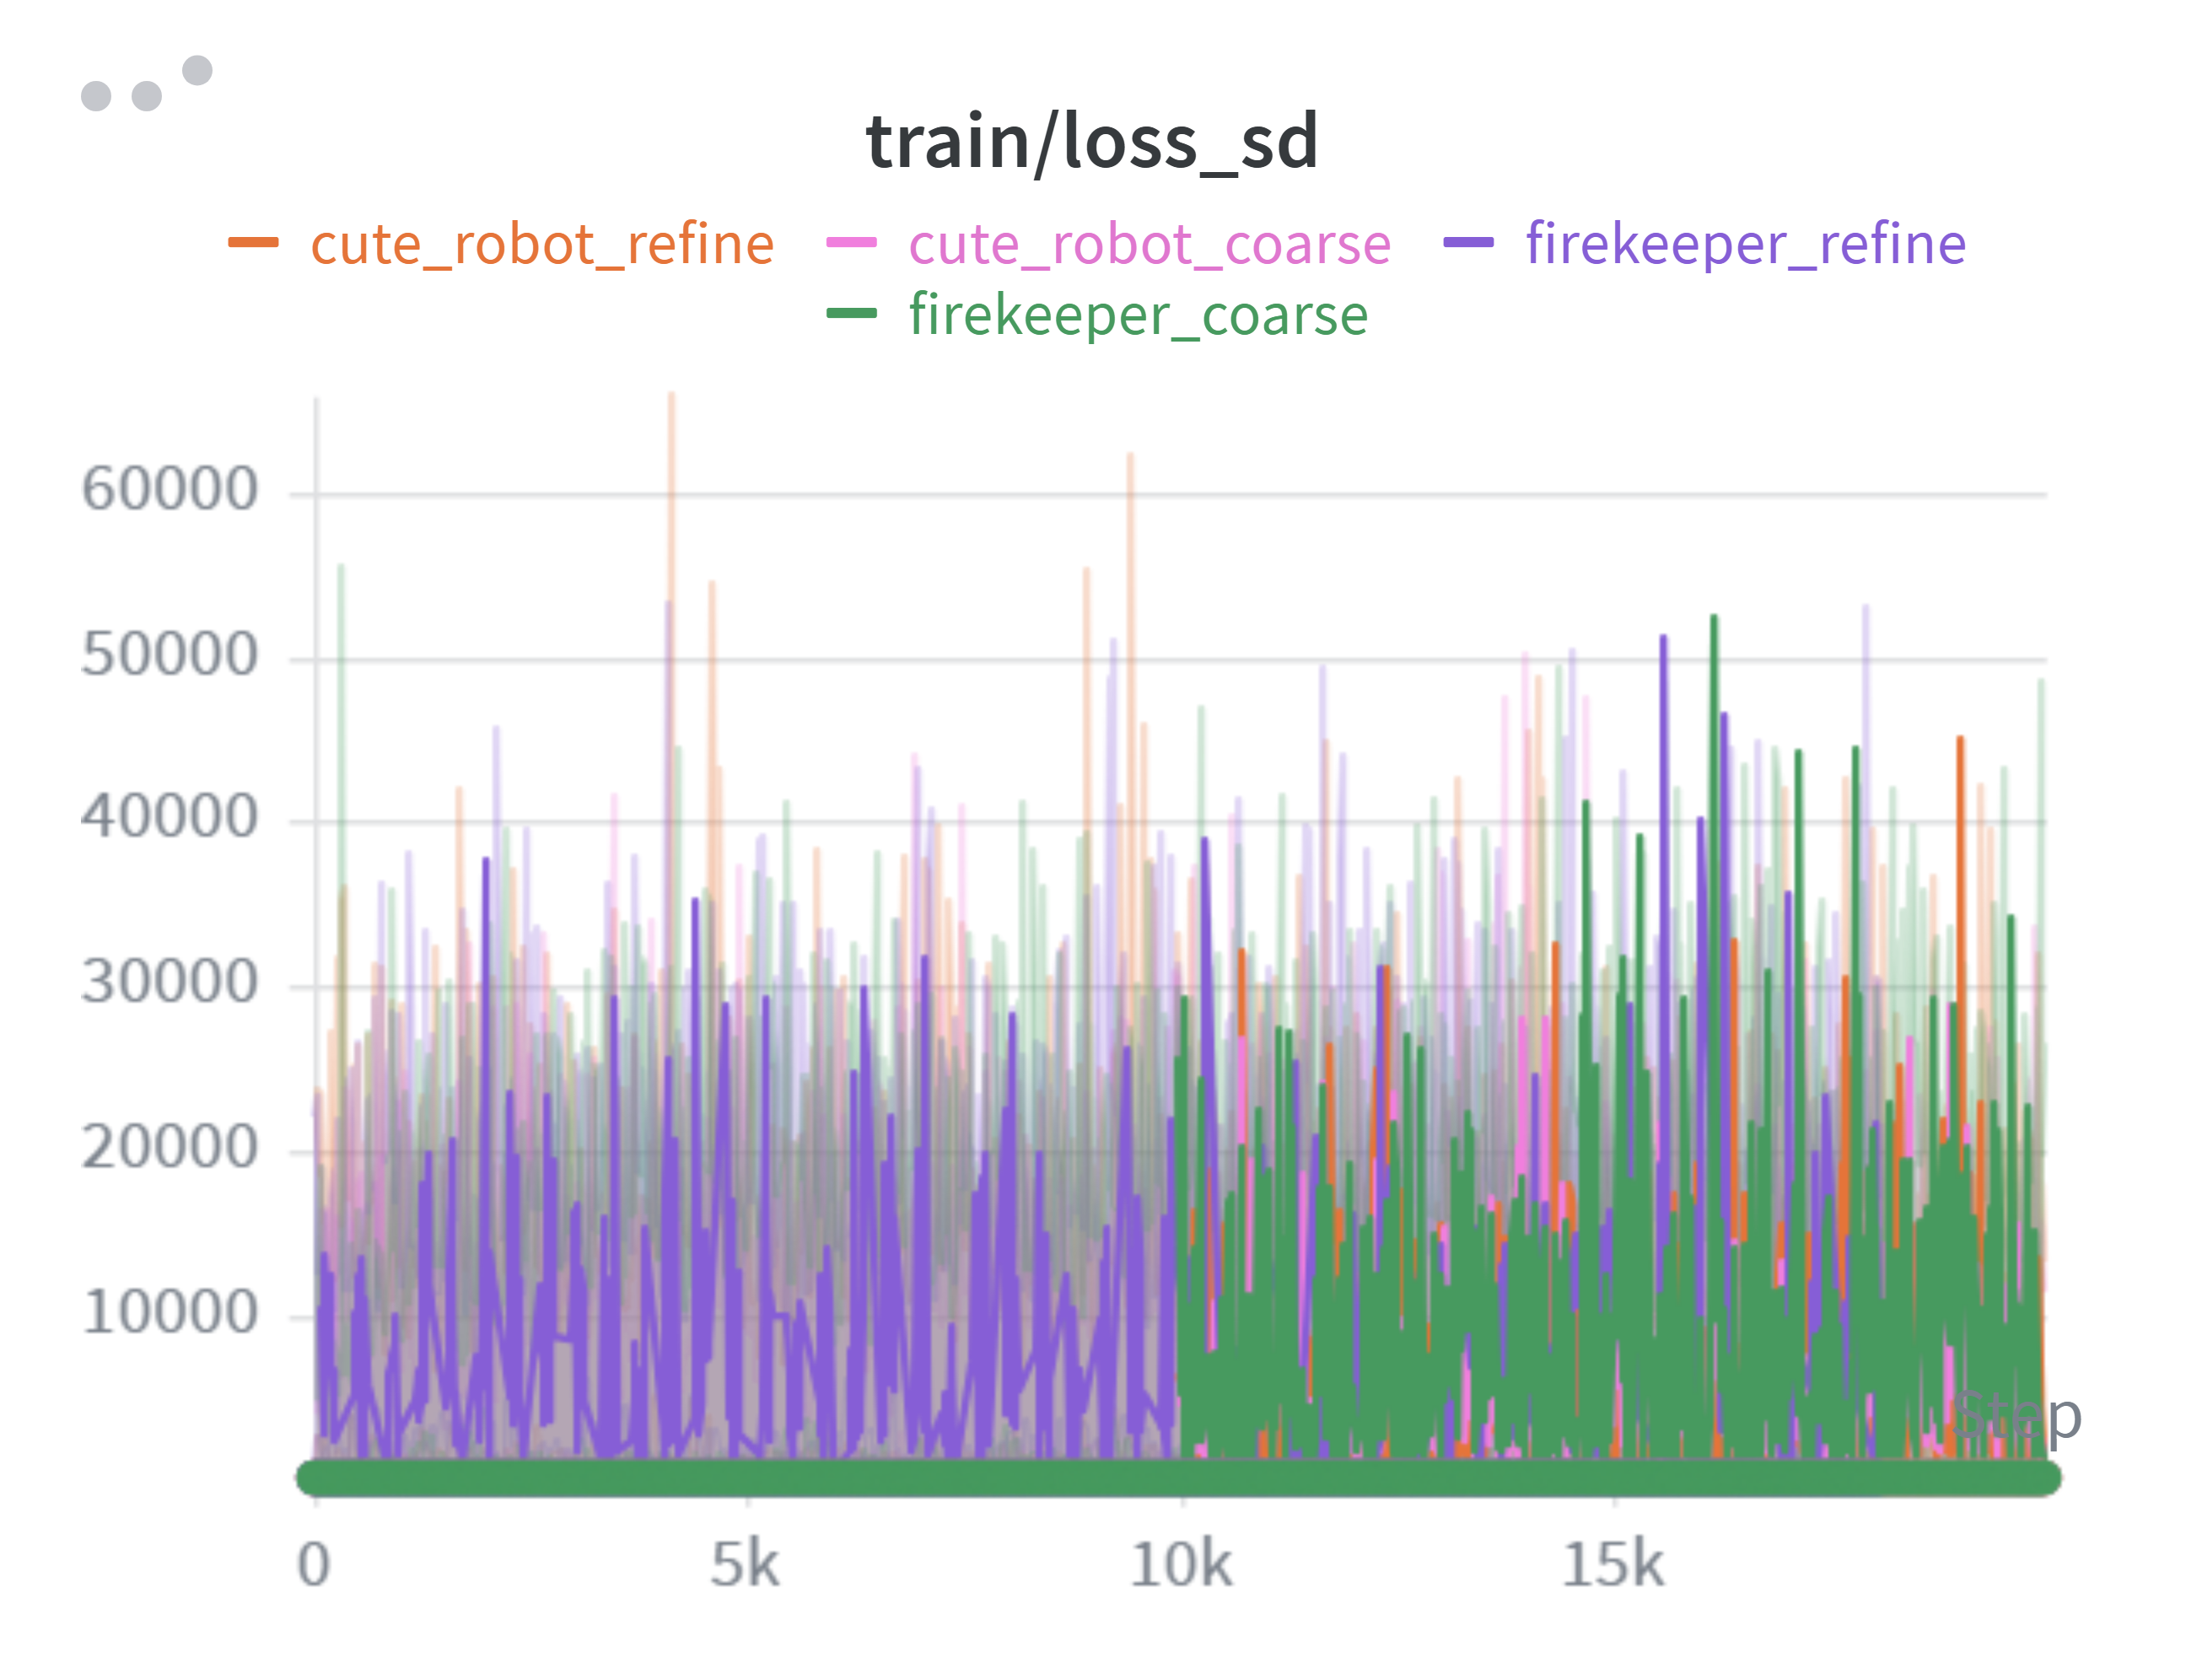
\includegraphics[width=\linewidth]{figures/task1/objectC/losses/loss_sd.png}
		\caption{SDS loss}
	\end{subfigure}
	\hfill
	\begin{subfigure}[t]{0.32\textwidth}
		\centering
		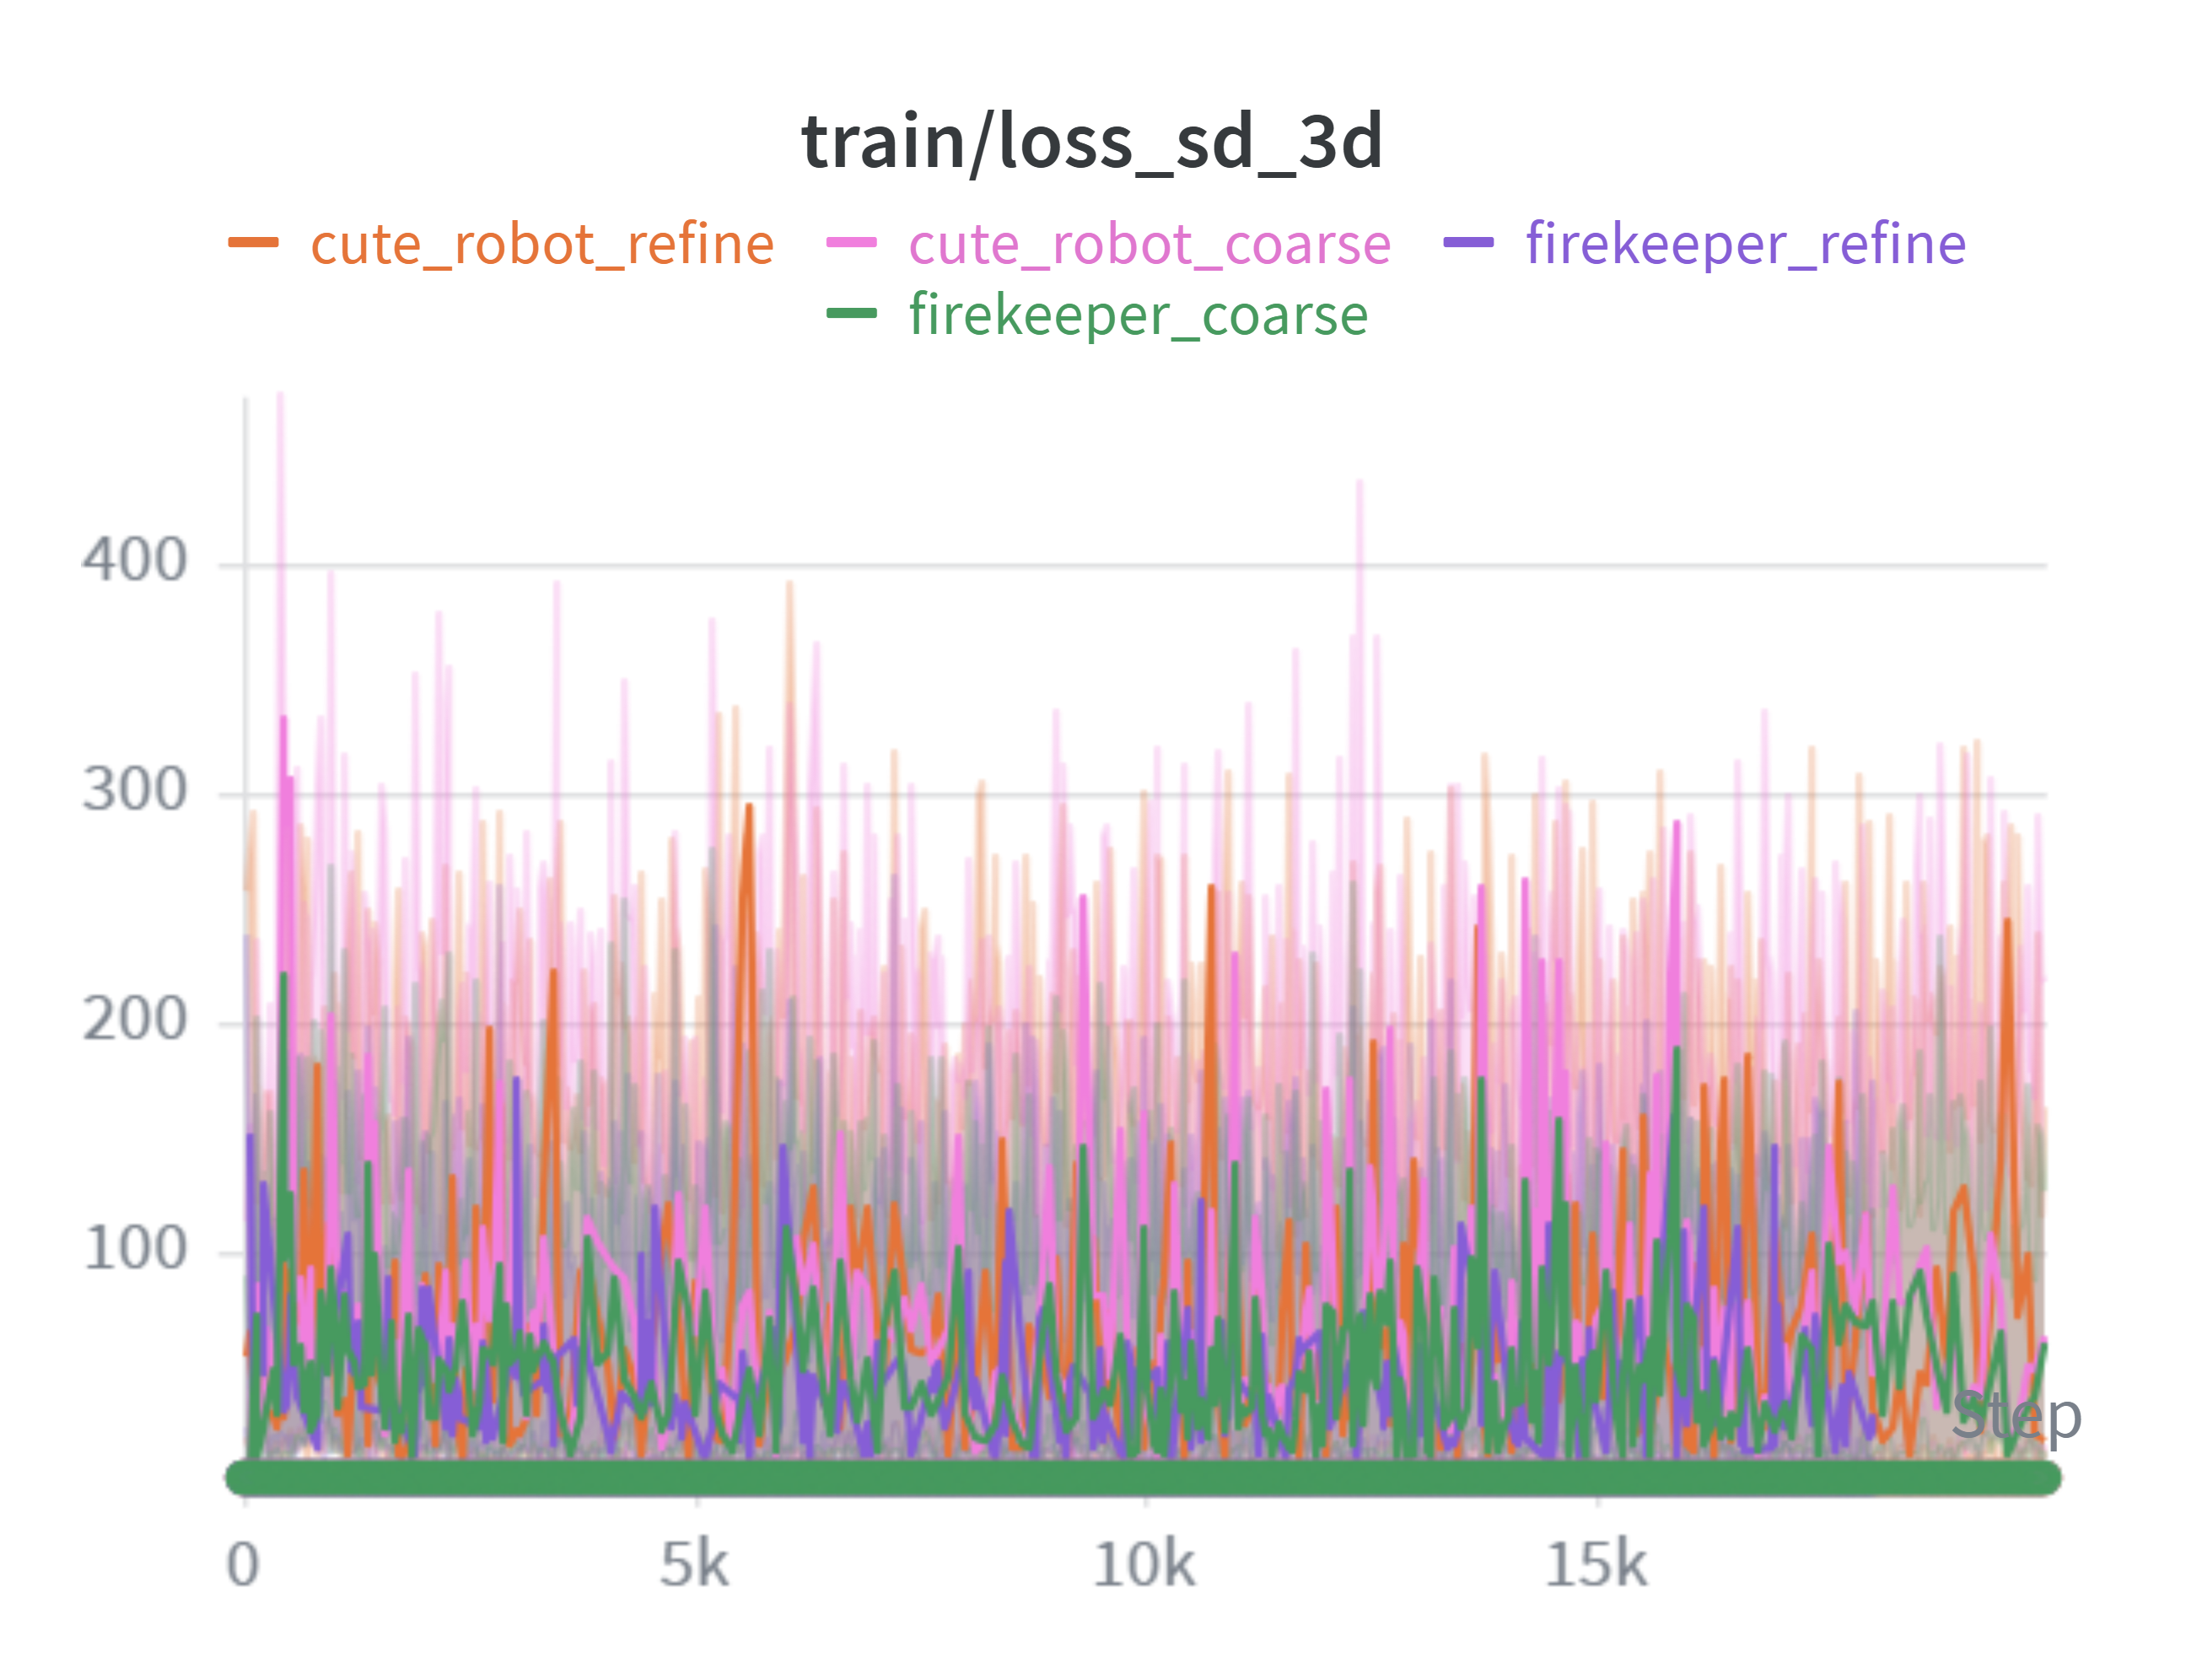
\includegraphics[width=\linewidth]{figures/task1/objectC/losses/loss_sd_3d.png}
		\caption{3D SDS loss}
	\end{subfigure}
	\hfill
	\begin{subfigure}[t]{0.32\textwidth}
		\centering
		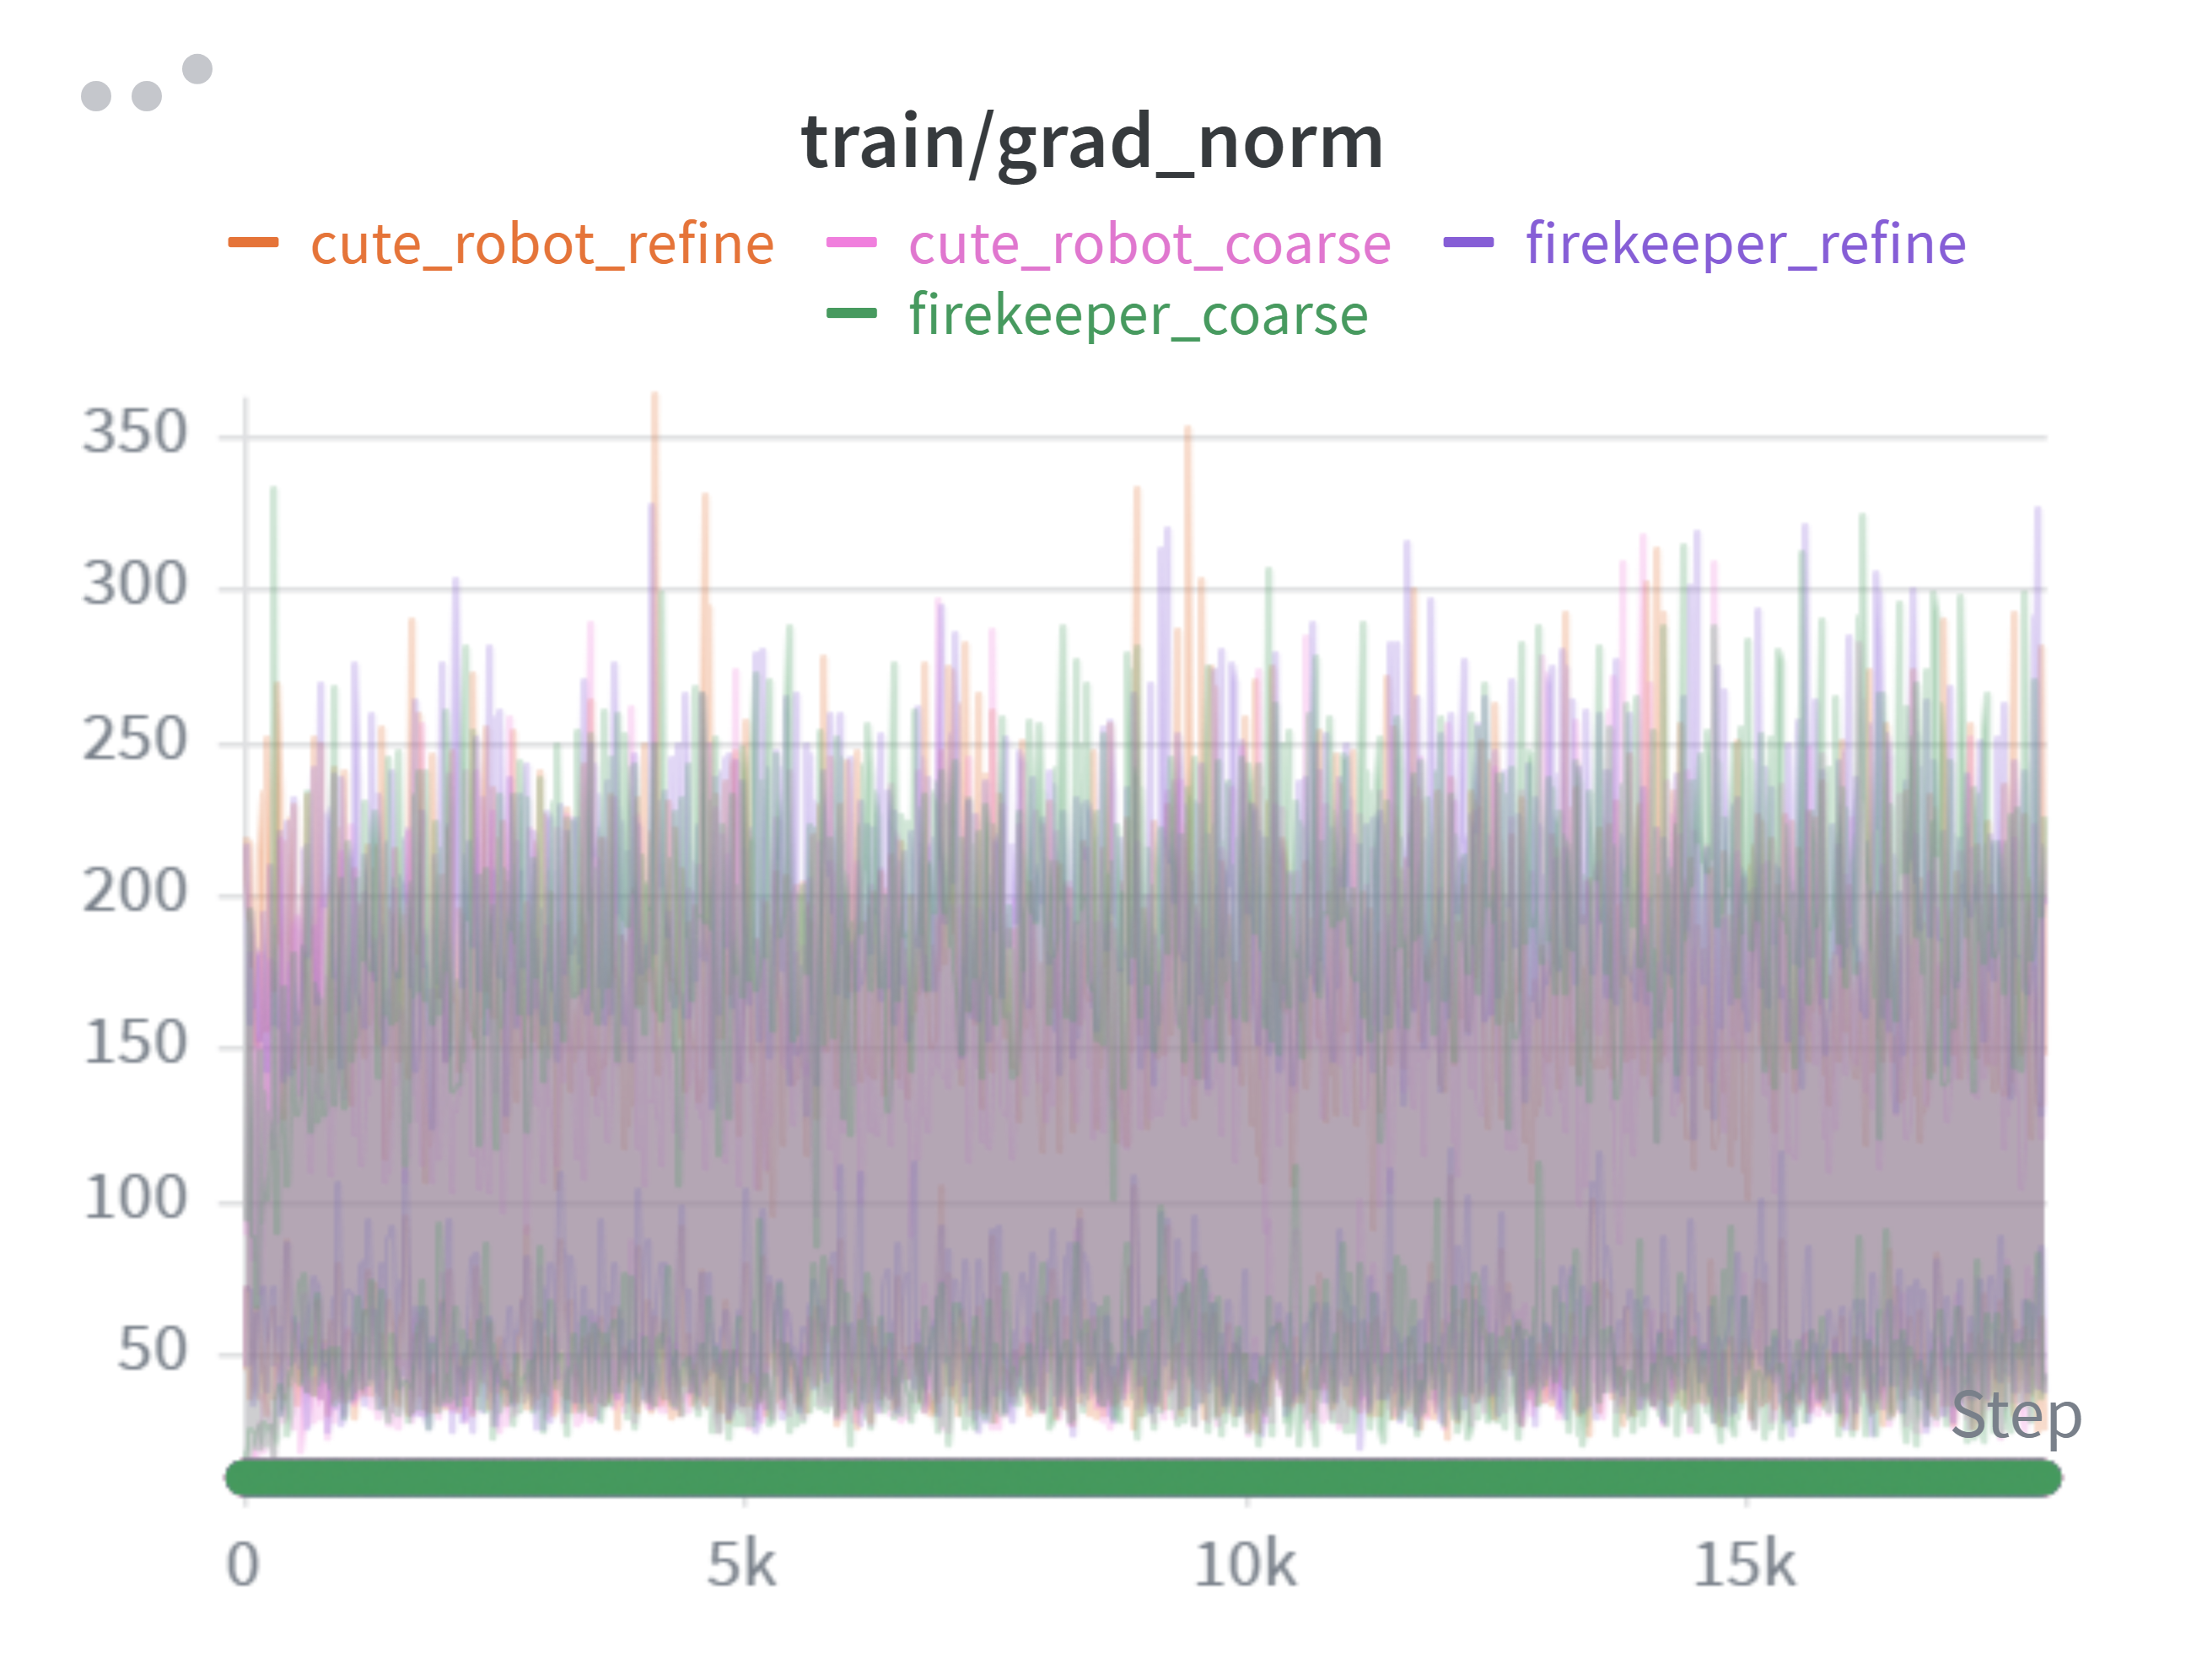
\includegraphics[width=\linewidth]{figures/task1/objectC/losses/grad_norm.png}
		\caption{Gradient norm}
	\end{subfigure}
	
	\vspace{0.5cm}
	
	%==================== 第二组：Regularization ====================
	\begin{subfigure}[t]{0.32\textwidth}
		\centering
		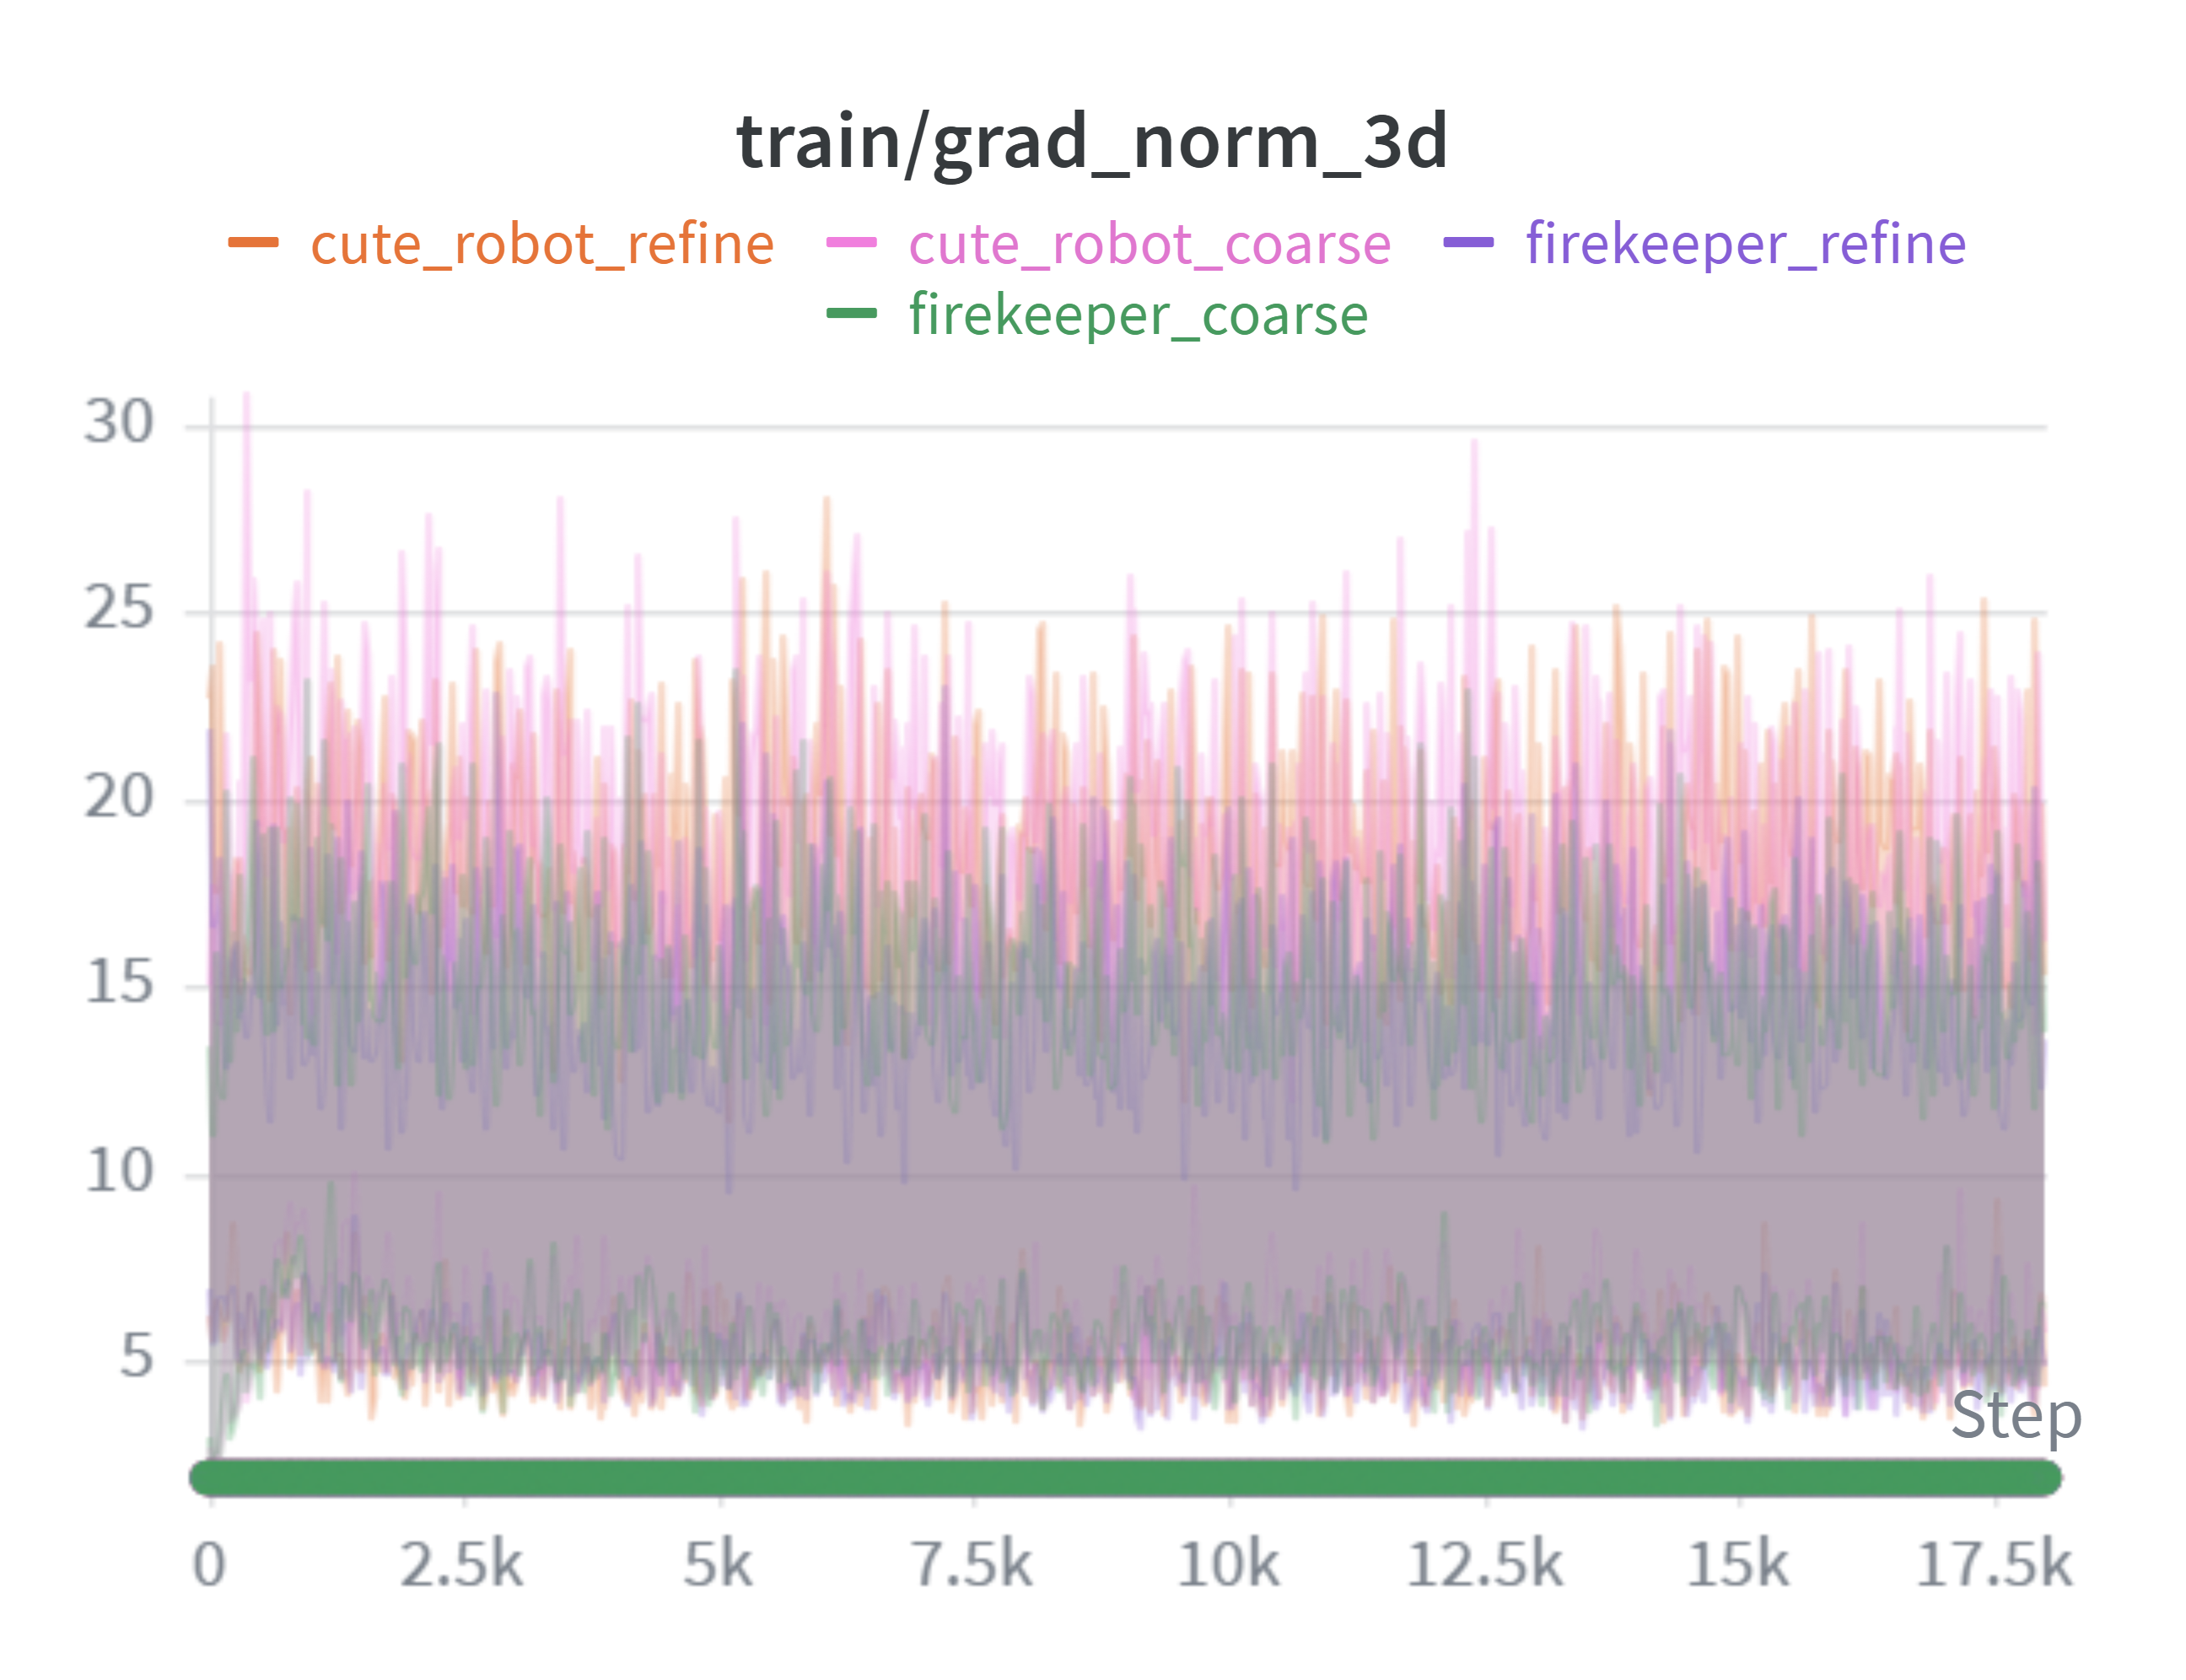
\includegraphics[width=\linewidth]{figures/task1/objectC/losses/grad_norm_3d.png}
		\caption{3D gradient norm}
	\end{subfigure}
	\hfill
	\begin{subfigure}[t]{0.32\textwidth}
		\centering
		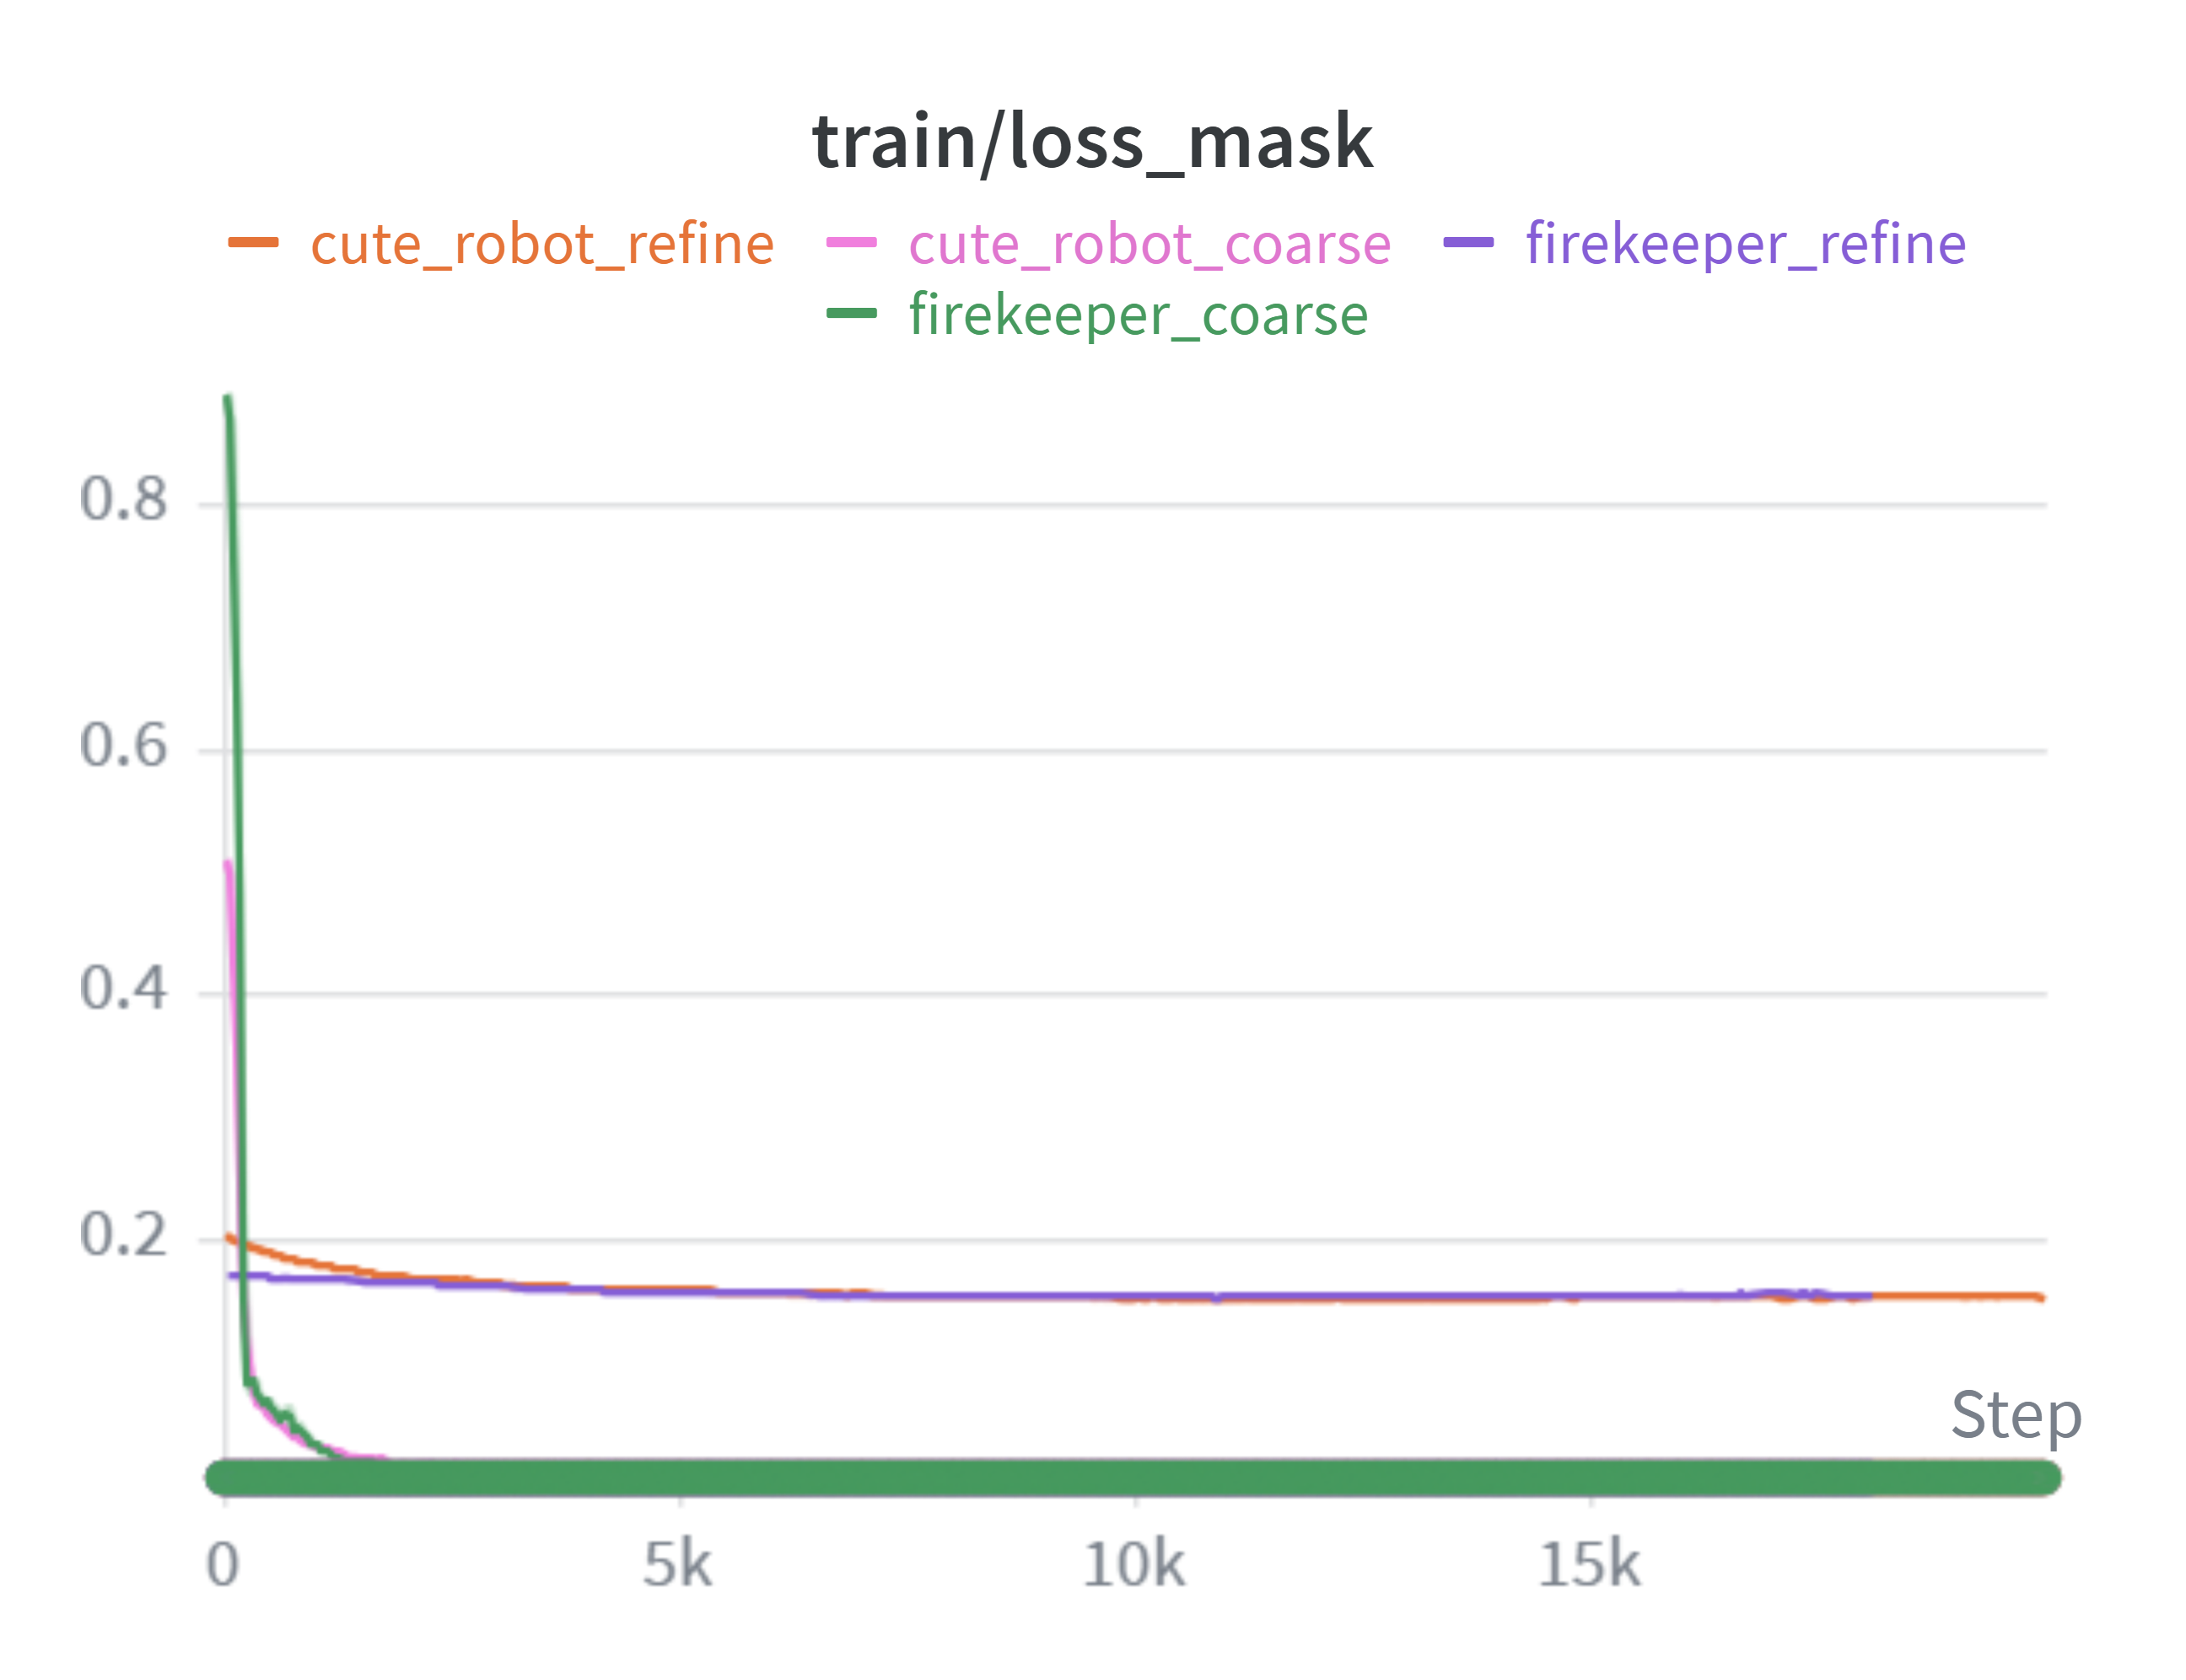
\includegraphics[width=\linewidth]{figures/task1/objectC/losses/loss_mask.png}
		\caption{Mask loss}
	\end{subfigure}
	\hfill
	\begin{subfigure}[t]{0.32\textwidth}
		\centering
		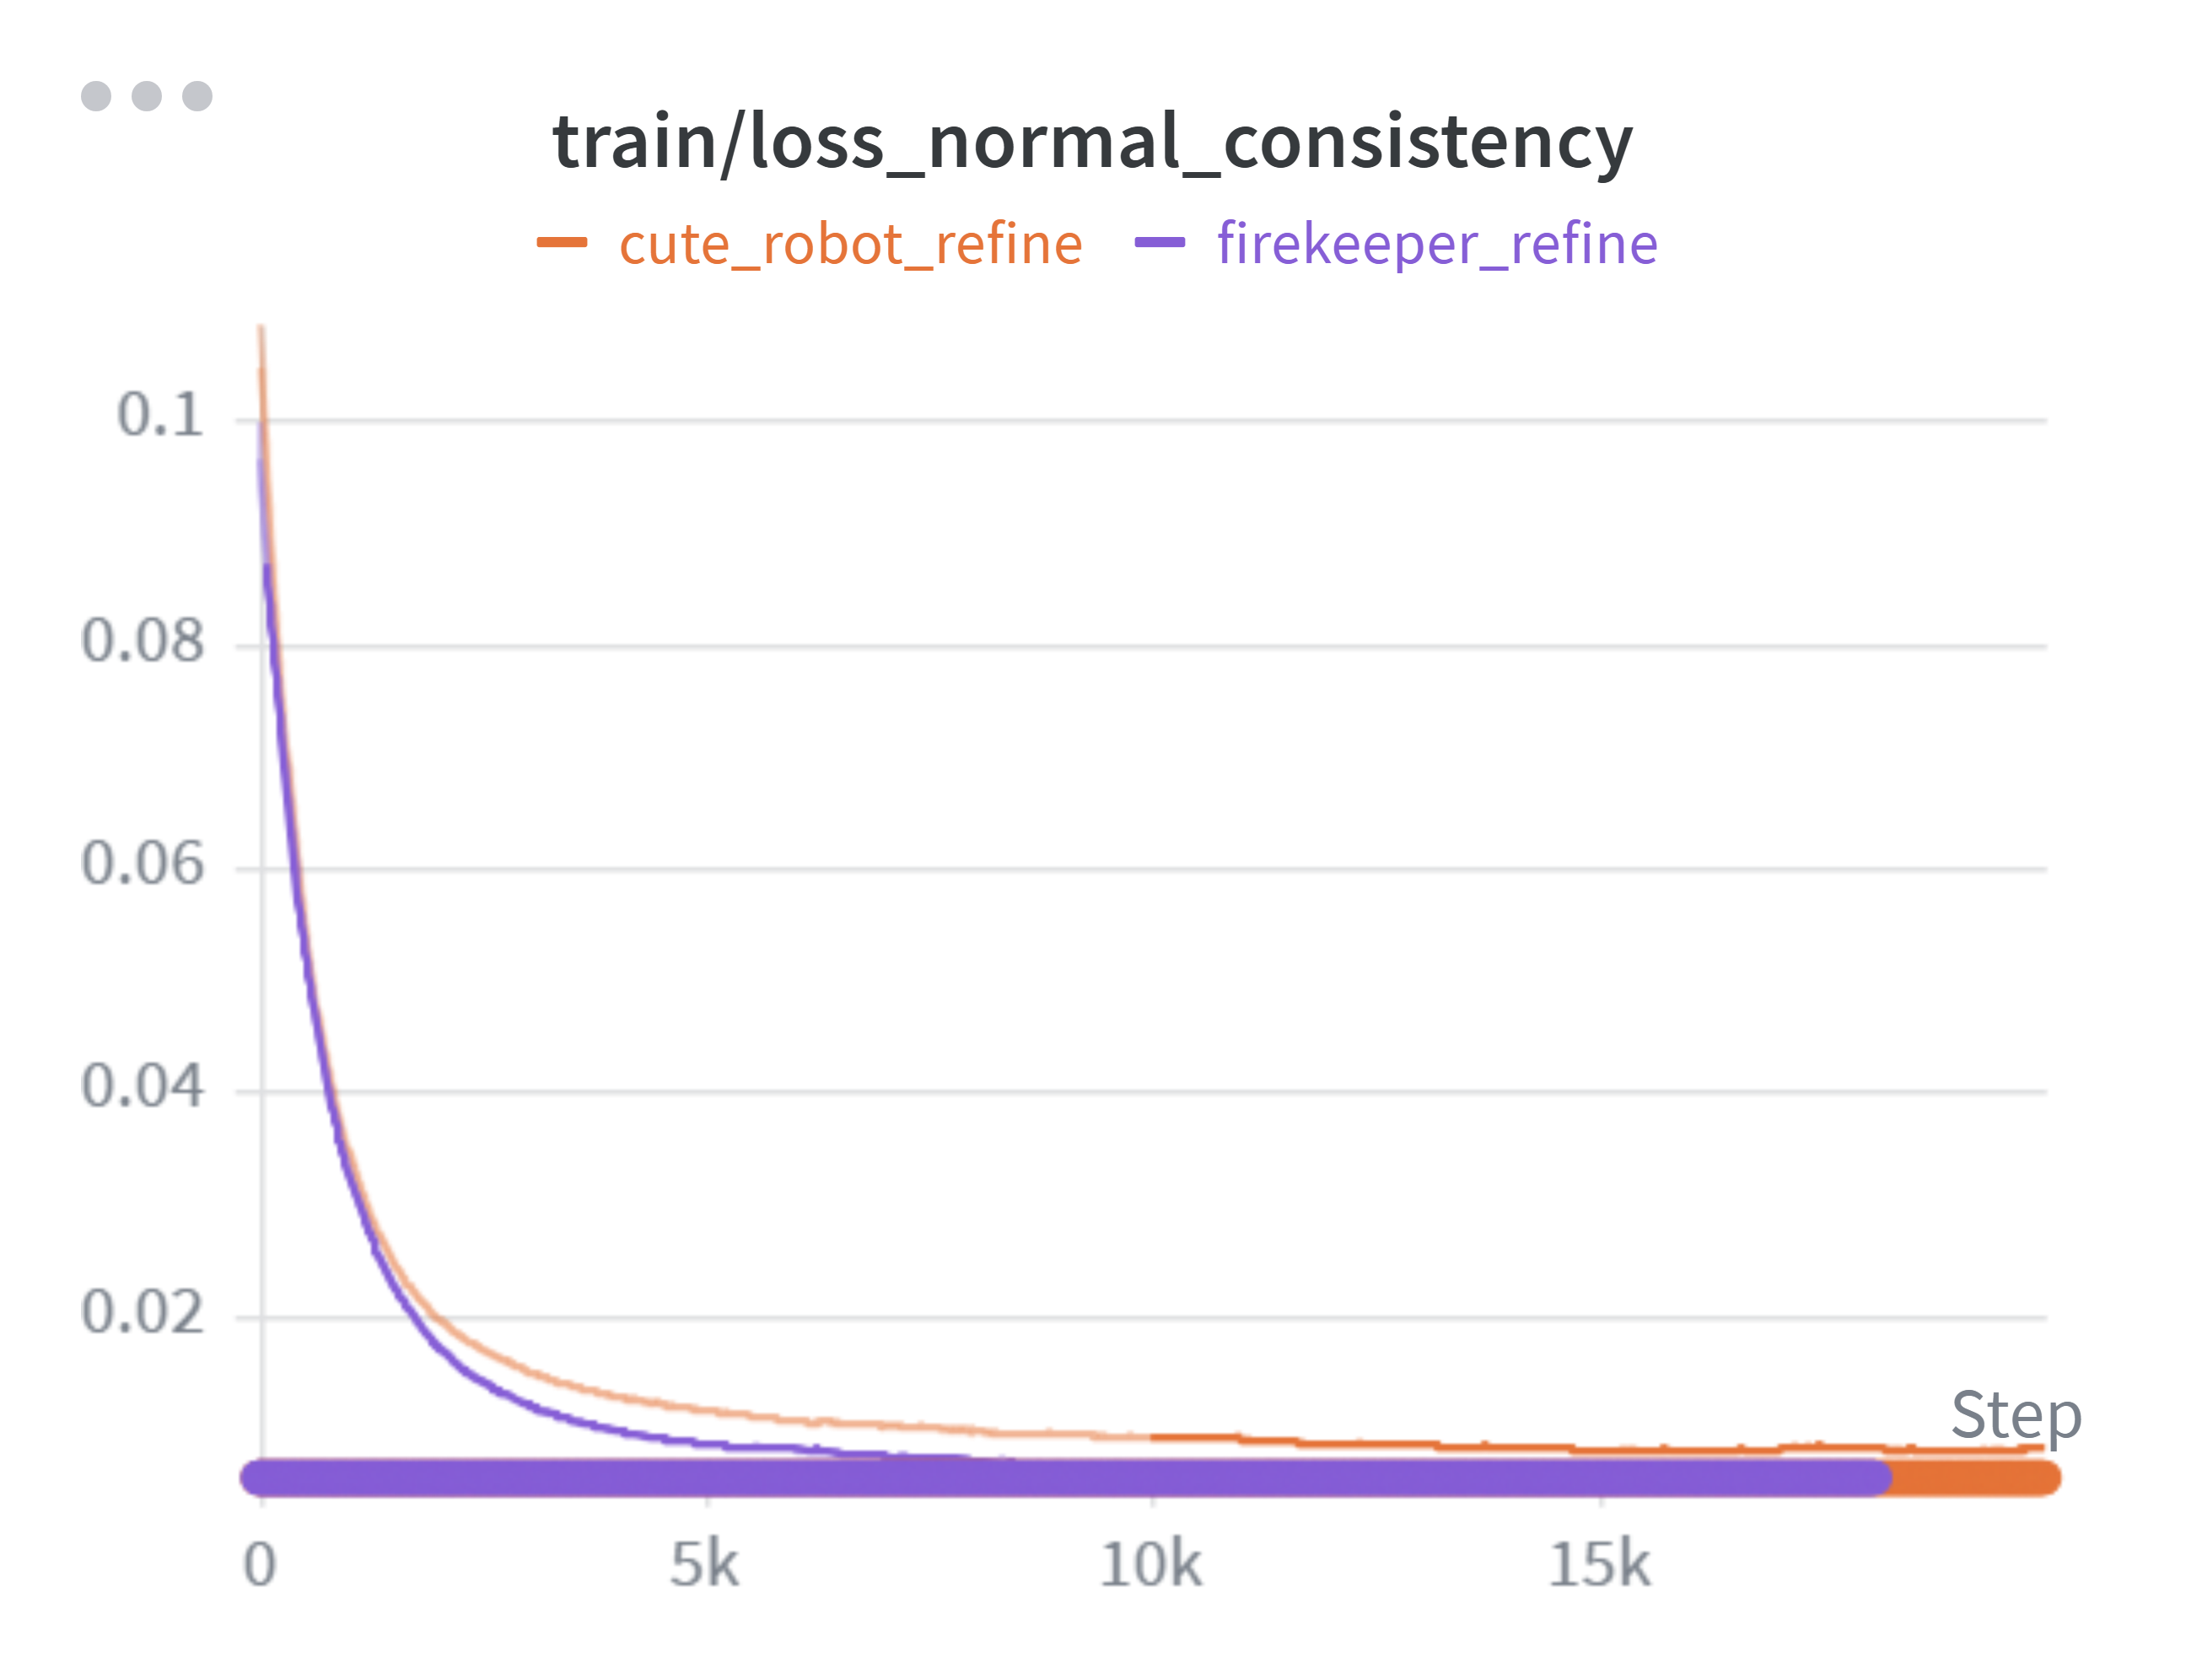
\includegraphics[width=\linewidth]{figures/task1/objectC/losses/loss_normal_consistency.png}
		\caption{Normal consistency loss}
	\end{subfigure}
	
	\vspace{0.5cm}
	
	%==================== 第三组：Reconstruction ====================
	\begin{subfigure}[t]{0.45\textwidth}
		\centering
		
\includegraphics[width=\linewidth]{figures/task1/objectC/losses/rgb_loss.png}
		\caption{RGB reconstruction loss}
	\end{subfigure}
	
	\caption{Training losses and optimization statistics for Object C.}
	\label{fig:objectC_losses}
\end{figure*}


We can see that the visualization results of both models have good and smooth shape and color distribution.

As for the training dynamics, here are our analysis:

Opaque Loss demonstrates a similar pattern as Object B, but with no obvious shakes. This may because the picture offers enough geometry features for the model so that it can easily build the rough but accurate outfit.

Sparsity Loss has a similar behavior as Object B.


The SDS Loss and 3D SDS Loss exhibit large fluctuations and high variance, which can be interpreted similarly as the SDS loss of Object B.

The gradient norm remains within a stable range overall. Although there are shakes, no persistent gradient explosion or vanishing occurs. This indicates that the training process is generally stable and the optimizer can effectively control parameter updates.

The Mask Loss decreases rapidly in the early stage of training and gradually converges to a low value, indicating that the model can quickly learn the separation between foreground and background regions, which helps improve the accuracy of geometric structures.

The Normal Consistency Loss exhibits a clear rapid decay trend, indicating that the normal consistency of the mesh surface continuously increases. This constraint effectively reduces local noise and discontinuous surfaces, making the generated results smoother.

The RGB Reconstruction Loss decreases and finally stabilizes, demonstrating that the model's texture and color reconstruction capabilities are continuously improving, and the difference between the rendered results and the target image keeps decreasing.


\subsection{Background Scene Visualization}
In this section, 185 pictures of garden(picking $\frac{1}{4}$ of the original resolution for efficiency) are trained. It takes about \textbf{1:12:42hour} to extract pose with COLMAP and \textbf{19:30min}(20000 epochs) to train.

One of the original pictures and the rendering results are as follow:
\begin{figure}[H]
	\centering
	

	\begin{subfigure}{0.25\textwidth}
		\centering
		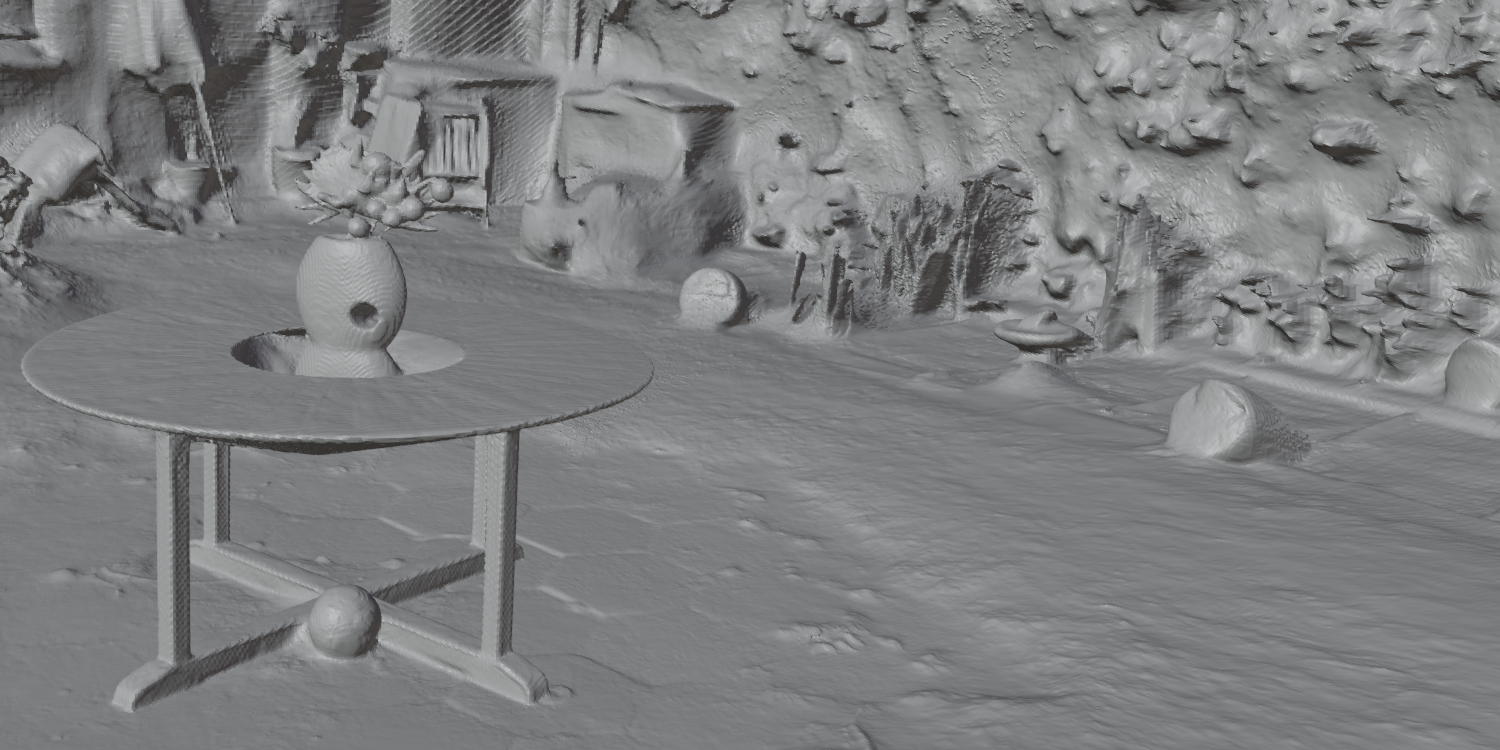
\includegraphics[width=\linewidth]{figures/task1/background/garden_mesh.png}
		\caption{Garden Mesh}
	\end{subfigure}
	\hfill
	\begin{subfigure}{0.25\textwidth}
		\centering
		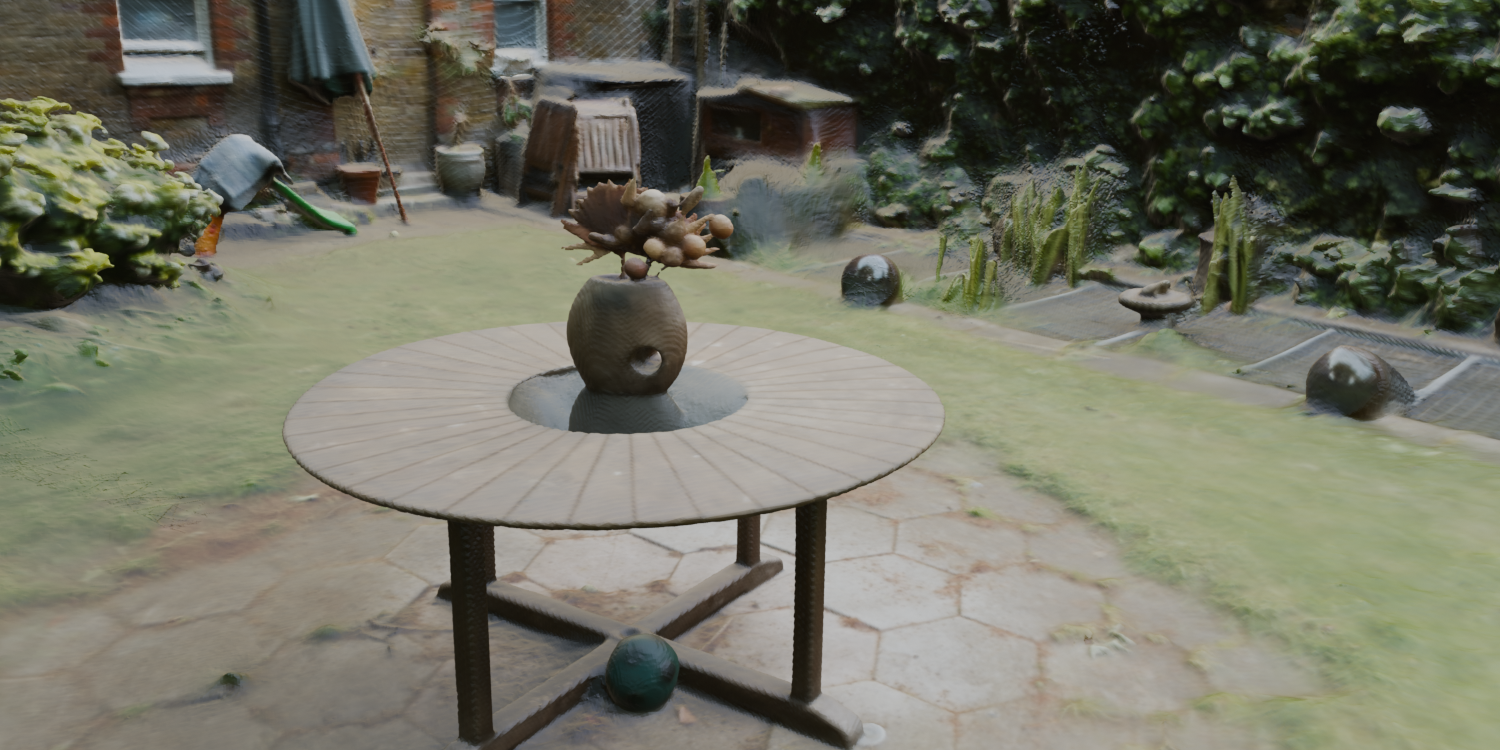
\includegraphics[width=\linewidth]{figures/task1/background/garden_color.png}
		\caption{Garden Color}
	\end{subfigure}
	\hfill
	\begin{subfigure}{0.25\textwidth}
		\centering
		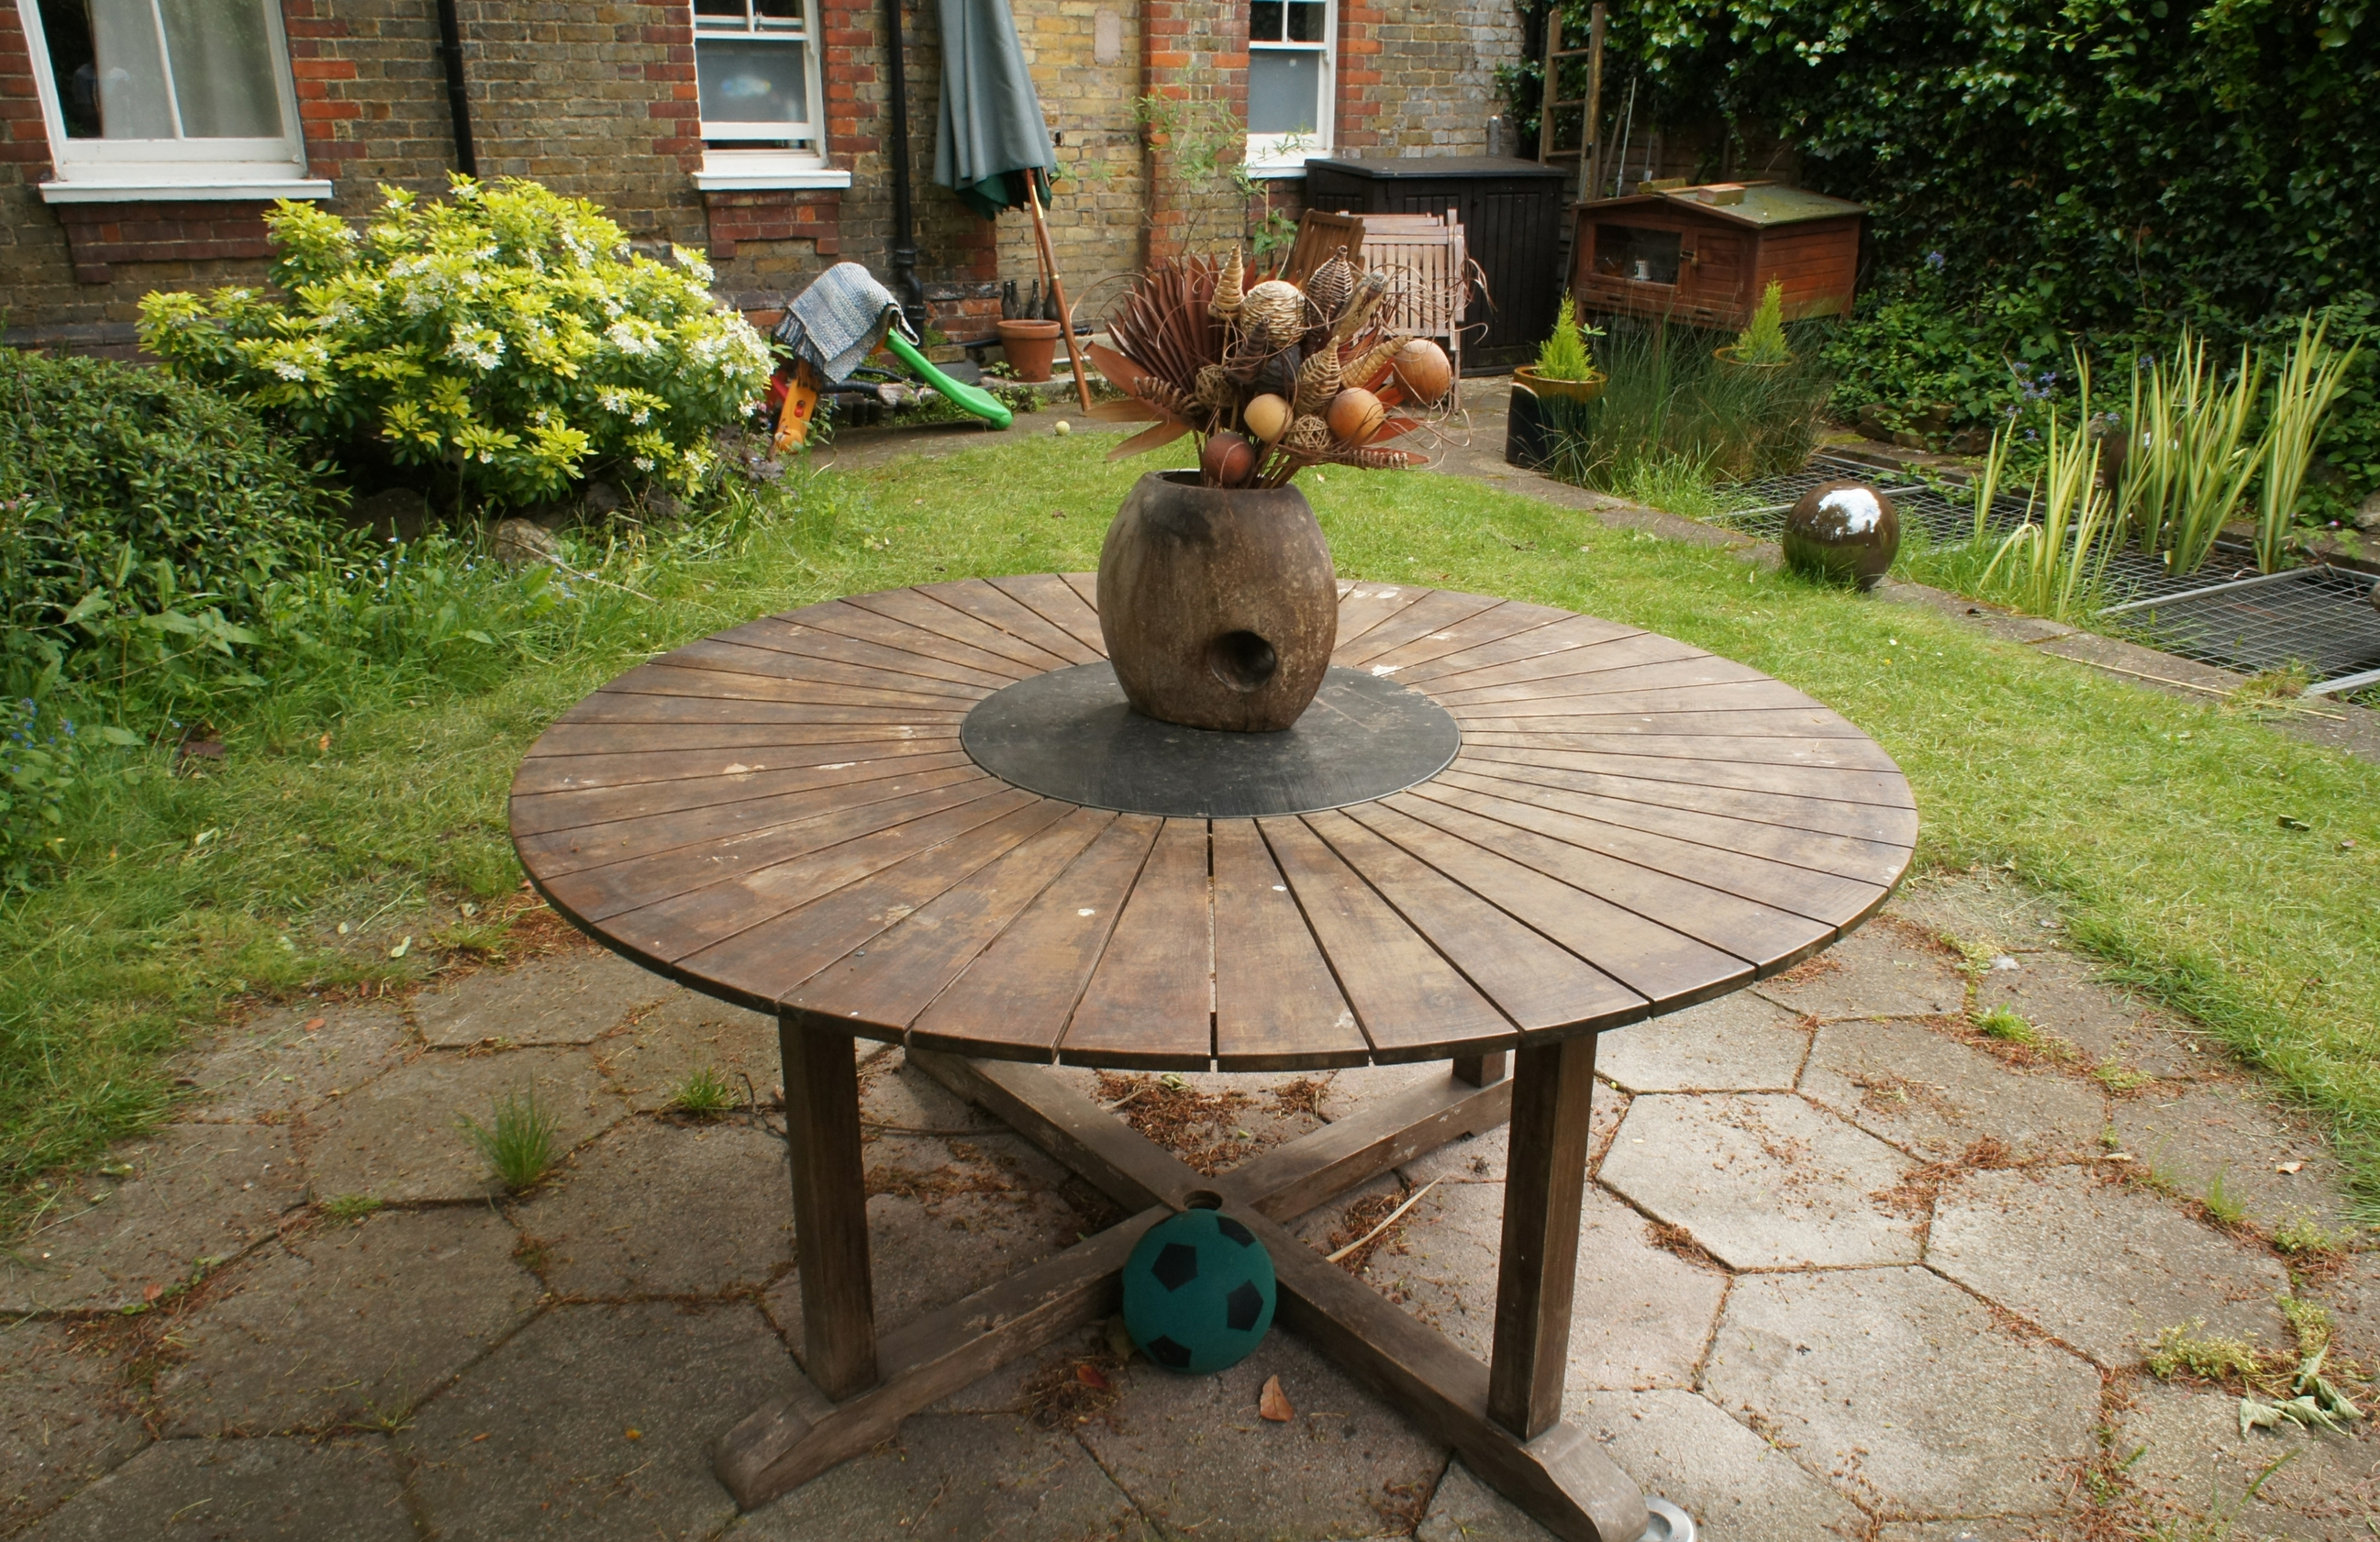
\includegraphics[width=\linewidth]{figures/task1/background/garden.jpg}
		\caption{Original Garden}
	\end{subfigure}
	
	\vspace{0.6cm}
	
	
\end{figure}
In this part, 2 meshes are exported(bounded and unbounded), where the unbounded mesh is in a form of a whole box. The box has an irregular outer shell and sky because these parts are not included in the images, while the rest of the model looks very good.


The detailed quality analysis will be shown later.



The training dynamics are as follow:

\begin{figure}[H]
	\centering
	
	% 第一行
	\begin{subfigure}{0.4\textwidth}
		\centering
		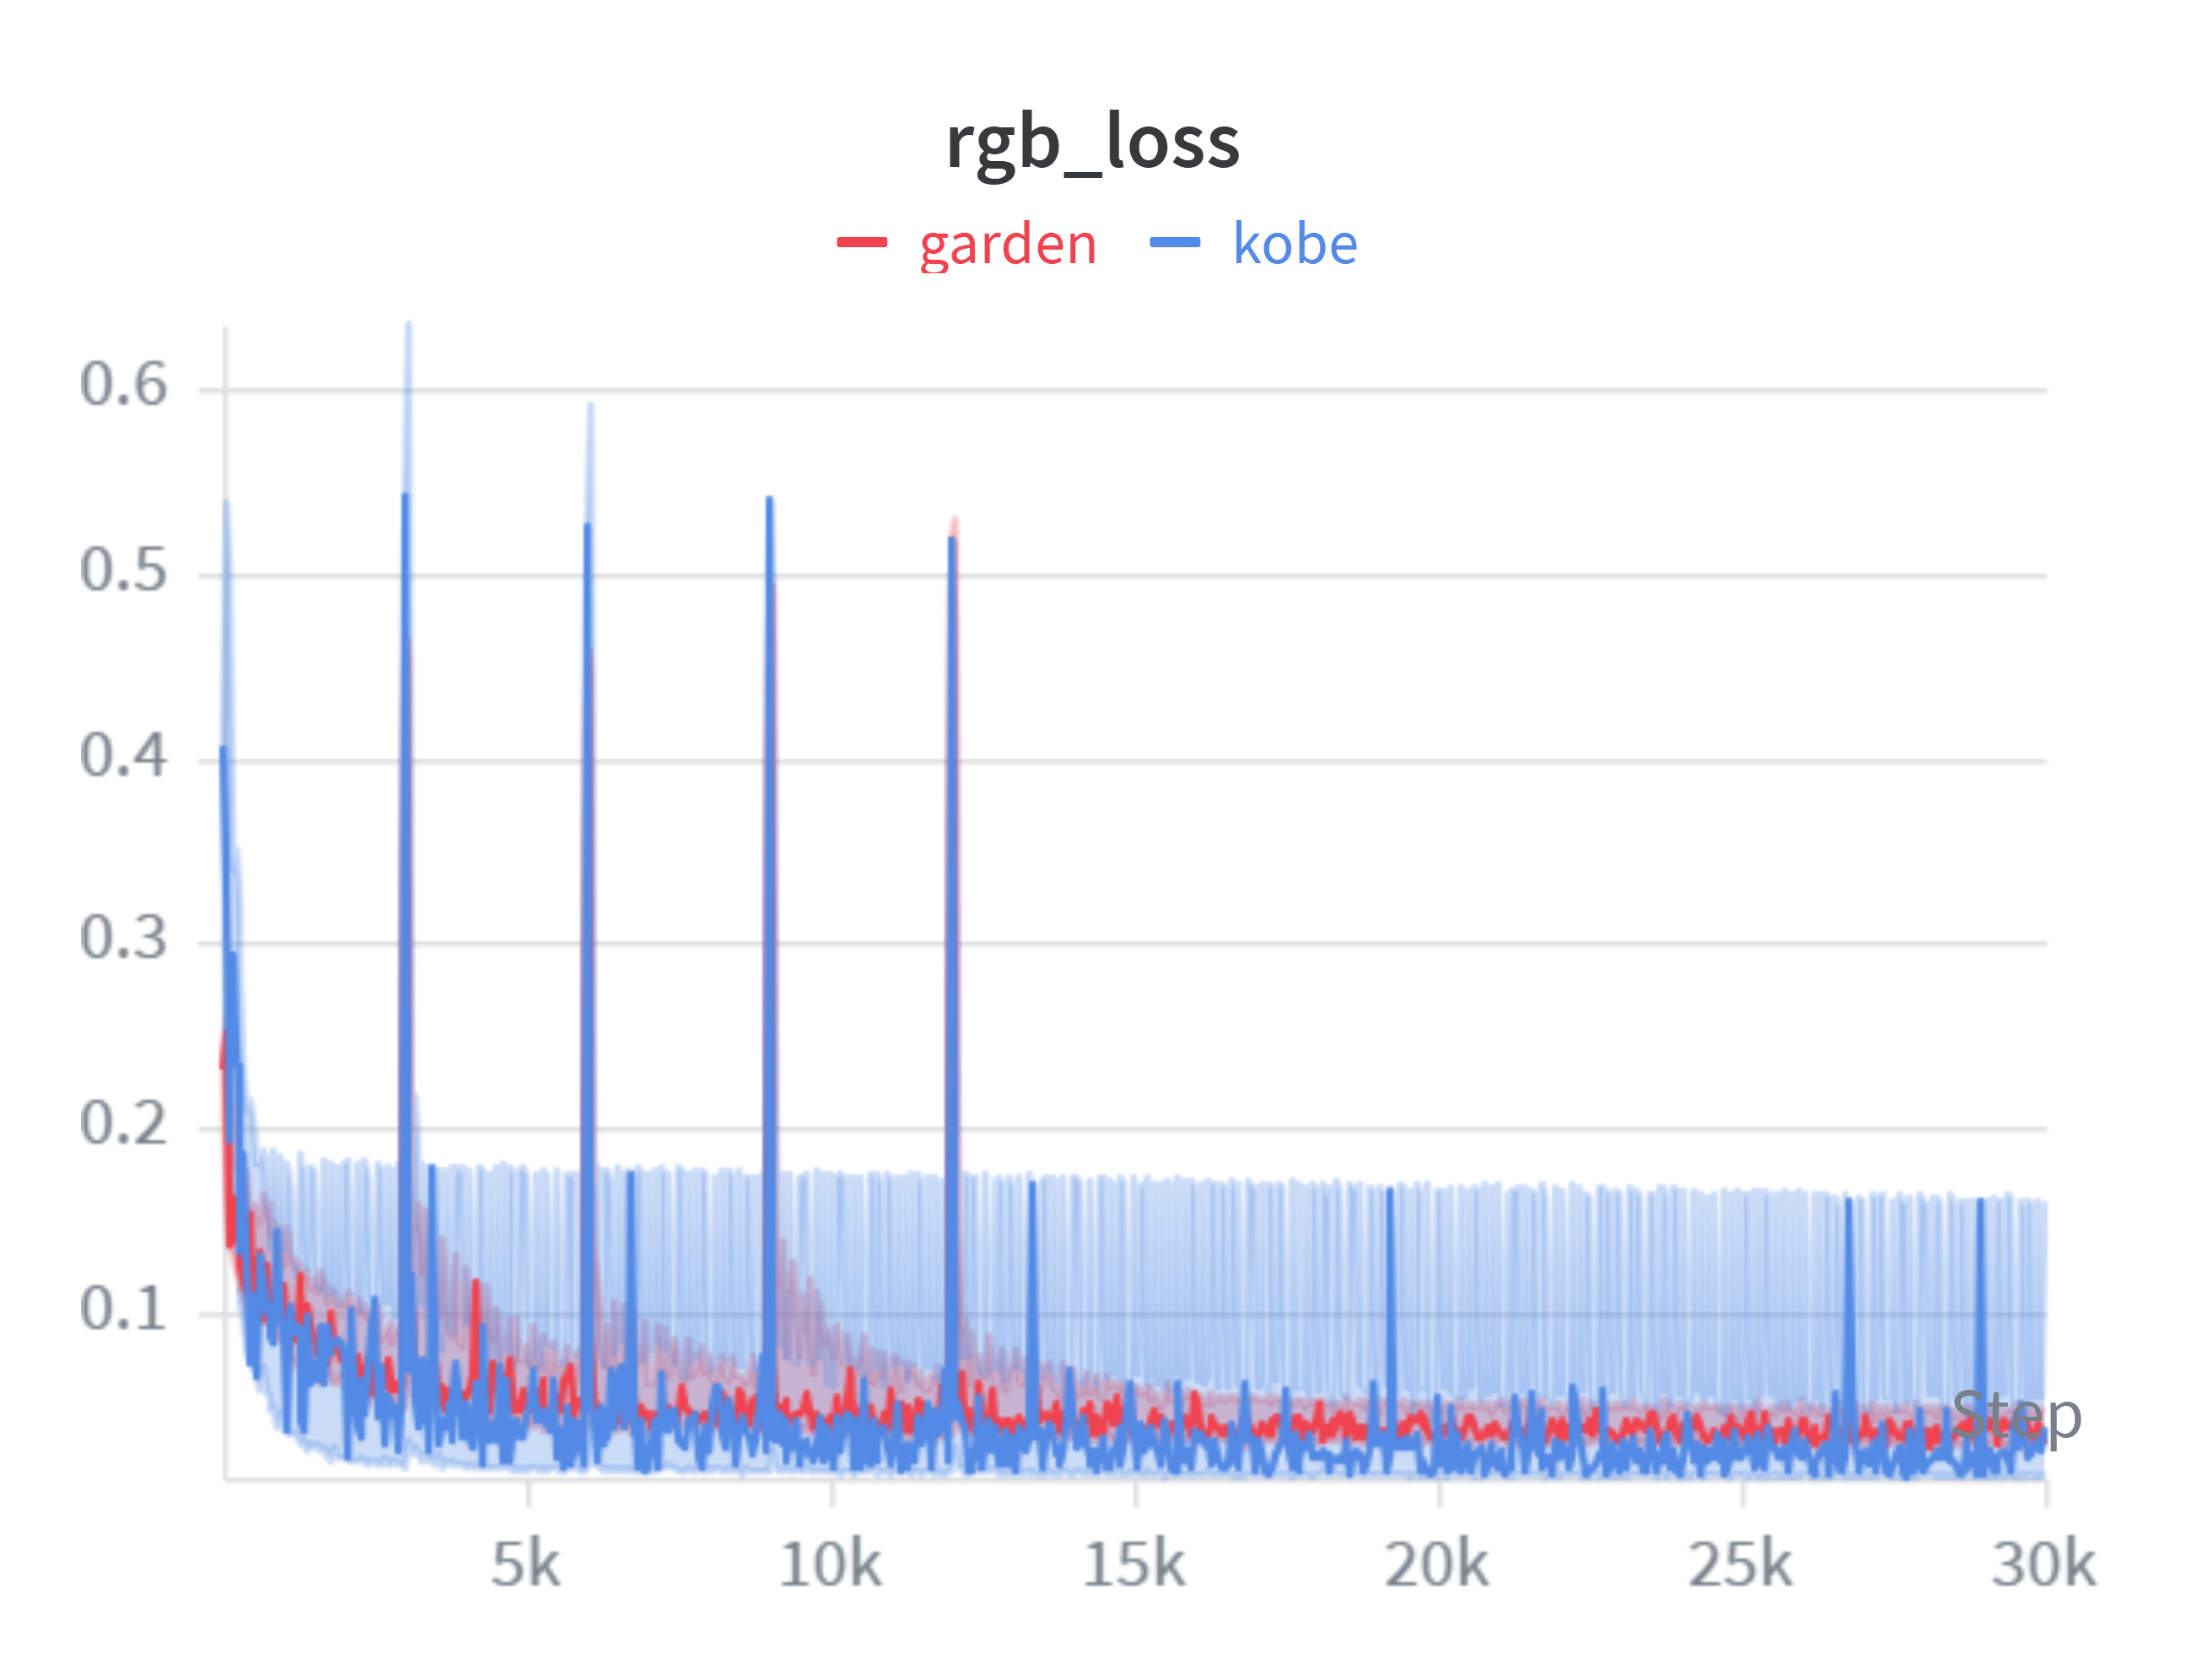
\includegraphics[width=\linewidth]{figures/task1/background/rgb_loss.png}
		\caption{RGB Loss}
	\end{subfigure}
	\hfill
	\begin{subfigure}{0.4\textwidth}
		\centering
		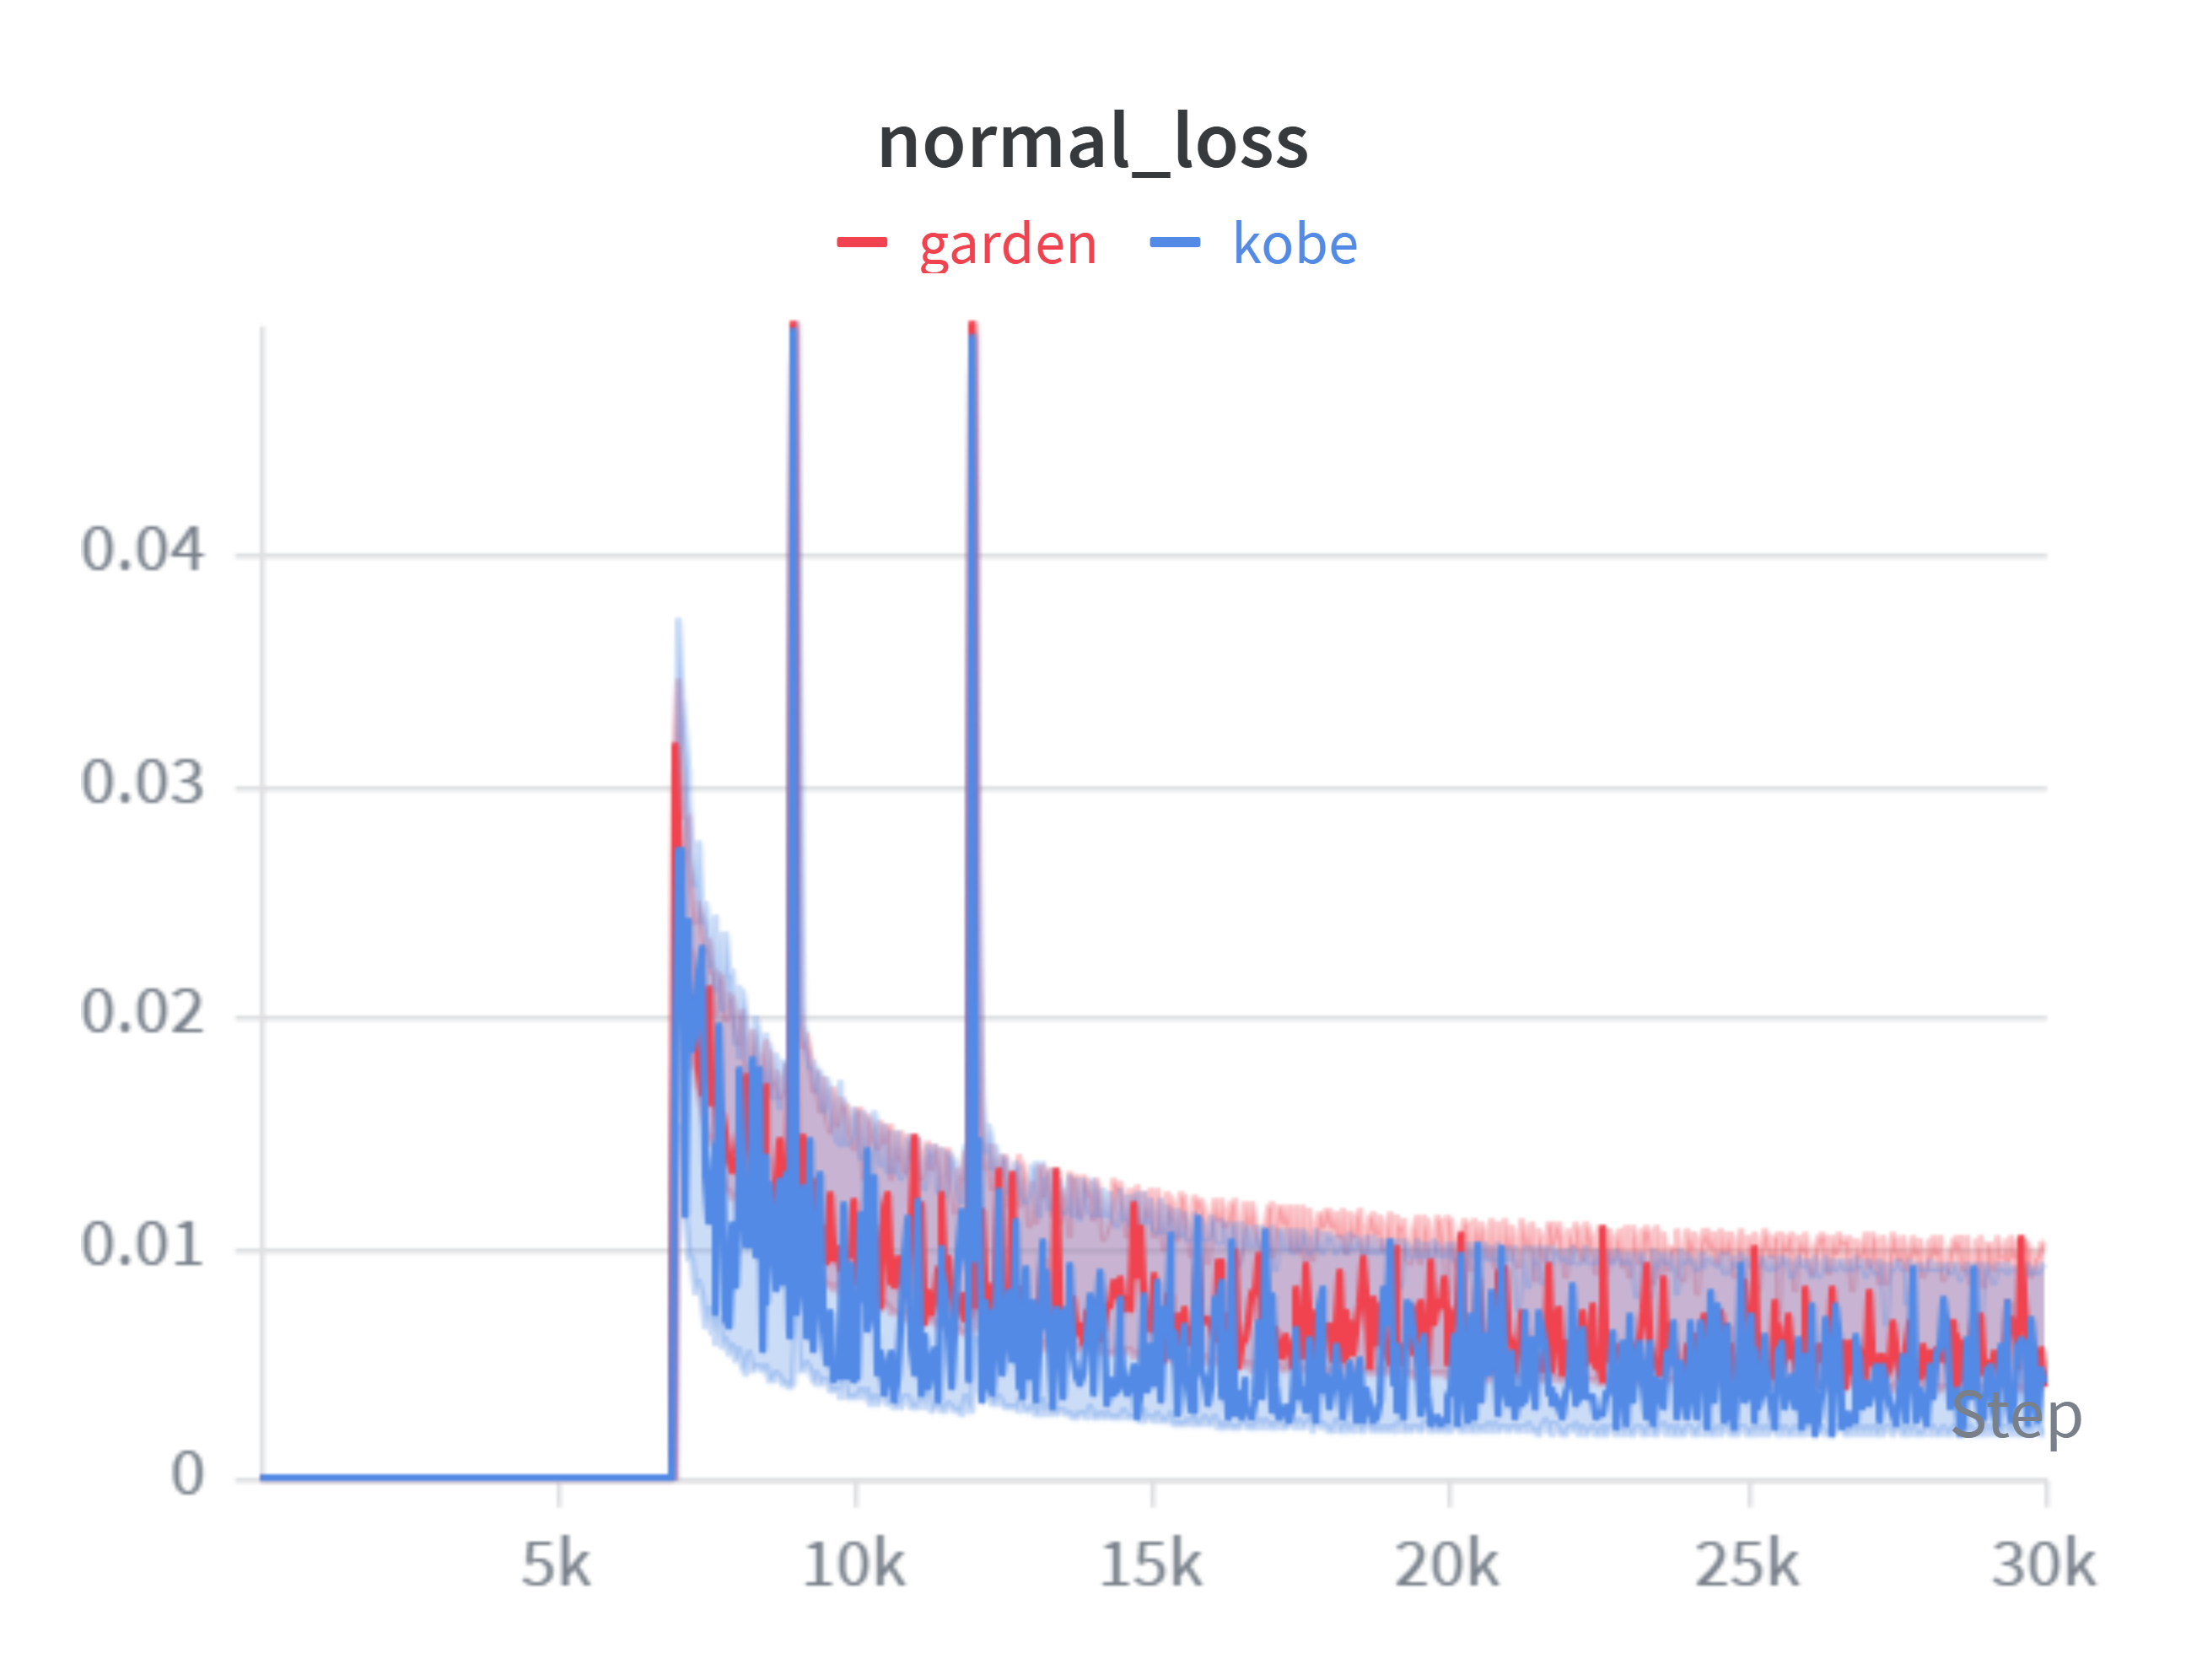
\includegraphics[width=\linewidth]{figures/task1/background/normal_loss.png}
		\caption{Normal Loss}
	\end{subfigure}

	
	\caption{Training Dynamics}
	\label{fig:2DGS Dynamics}

\end{figure}

Both loss curves generally show a downward trend, and the red curve (Garden) is more stable and has fewer peaks than the blue curve (Kobe). This is likely because the Garden has 185 images, twice the dataset of Kobe, thus capturing color and normal information more accurately. Also, Garden captures way more feature points after COLMAP as is shown in Figure~\ref{figure:Feature Points}





\subsection{Quality Accessment}
In this part, all the 3D resources' quality are compared from different perspectives.
\subsubsection{Quantitative indicators}
\begin{table}[H]
	\centering
	\caption{Quantitative Evaluation of Reconstructed Objects and Background}
	\begin{tabular}{c|c|c|c|c}
		\hline
		\textbf{Object} & \textbf{PSNR $\uparrow$} & \textbf{SSIM $\uparrow$} & \textbf{LPIPS $\downarrow$} & \textbf{Training Time(min)} \\
		\hline
		A-Kobe   & 30.94 & 0.9569 & 0.2245 & 55 \\
		\hline
		B-Astronaut & - & - & - & 20 \\
		B-Bunny  & - & - & - &  20\\
		\hline
		C-Firekeeper & 11.669 & 0.1588 & 0.5905 &  60\\
		C-Robot & 8.5543 & 0.5913 & 0.4767 &  60\\
		\hline
		BG-Garden & 30.31 & 0.9080 & 0.1242 & 92 \\
		\hline
	\end{tabular}
	\label{tab:quantitative_results}
\end{table}

In this section, PSNR(Peak Signal-to-Noise Ratio),SSIM(Structural Similarity Inde),LPIPS(Learned Perceptual Ima`ge Patch Similarity) are introduced to access the quality of models. Specifically, Object Bs have no ground truth picture, so we didn't access them this way. \textbf{Also, Object Cs have only 1 picture and the rendering image is manually generated by us, so the accessment is not accurate and can only be taken for reference.}

We can see that Object A and Background Garden have obsessive advantages over Object Cs in geometry accuracy and  mesh details.


For the training time, Object B is the fastest, Object Cs all takes about an hour.
Specifically, Object A(COLMAP+2DGS) is variable.


Considering the training dynamic of Figure~\ref{figure:Feature Points}. We can see that the Garden has 128395 points compared with 5829 points of Kobe at the beginning of the training. This is because of the huge and high resolution dataset of Garden,which helps capture massive amounts of points during the COLMAP part. This takes time(1:12:42hour), but allows faster 2DGS(19:30min). 
\begin{figure}[h]
	\centering
	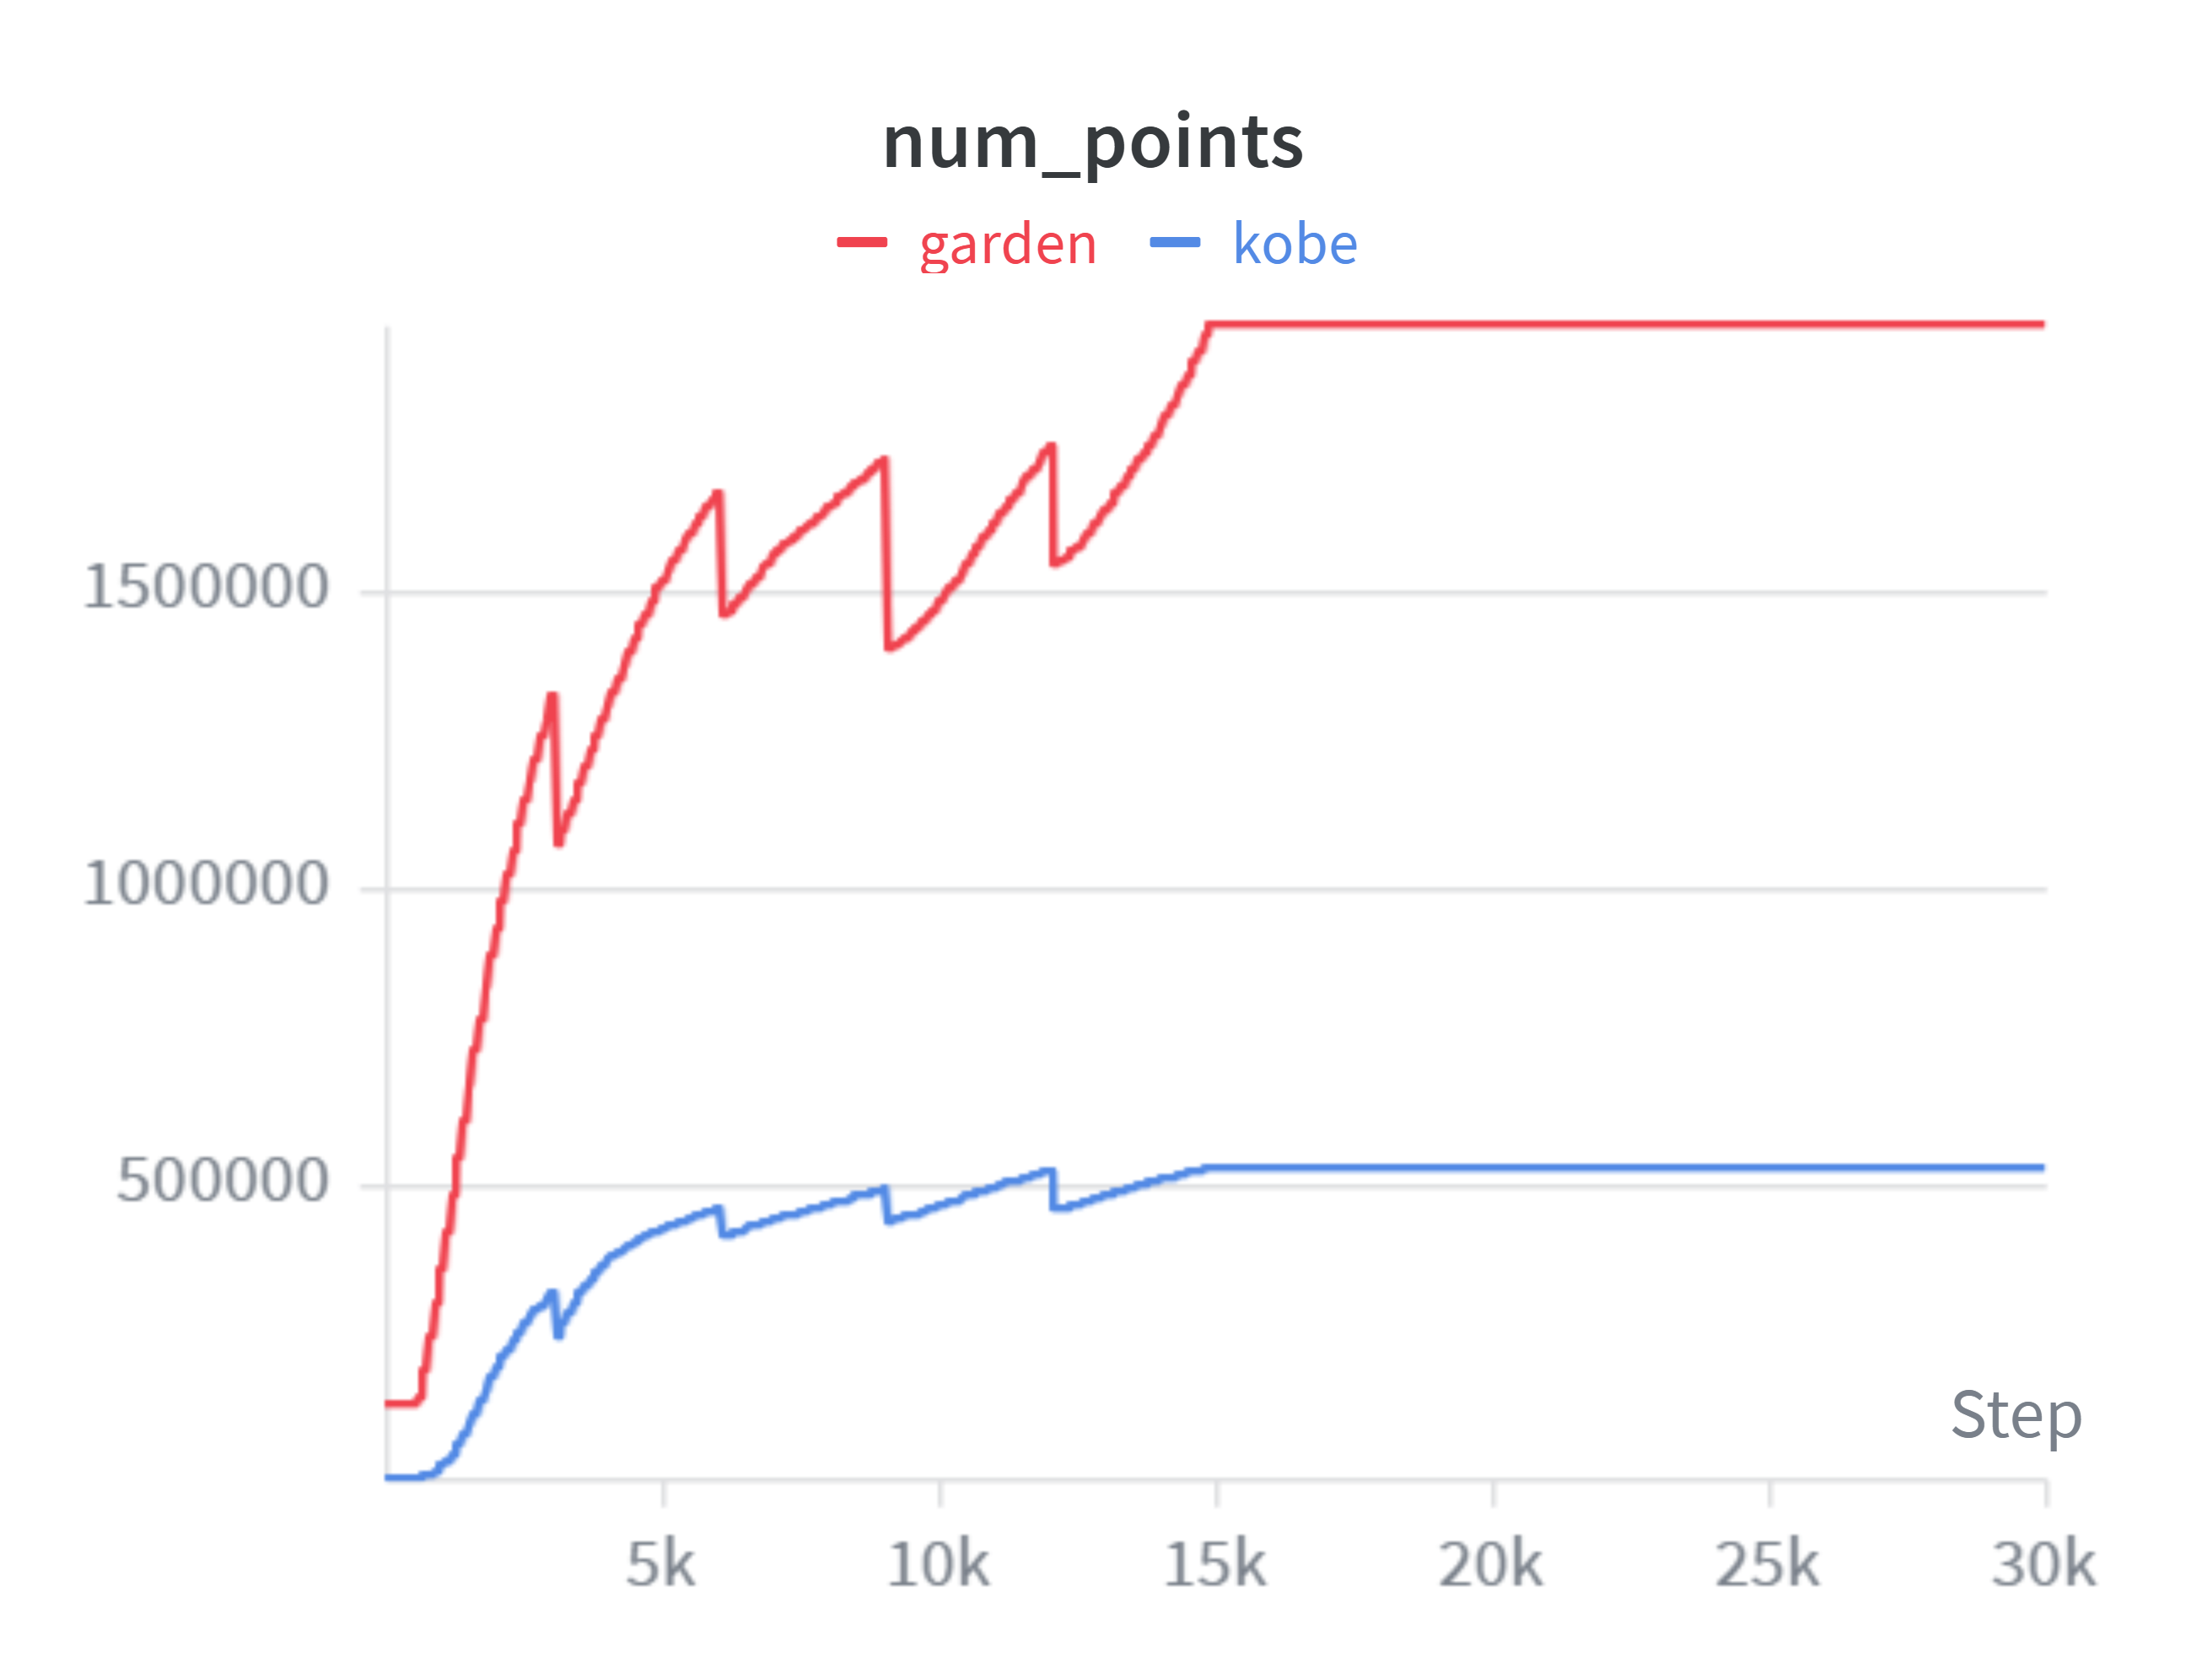
\includegraphics[width=0.4\linewidth]{figures/task1/background/num_points.png}
	\caption{Feature Points}
	\label{figure:Feature Points}
\end{figure}	


\subsubsection{Visual Evaluation}
Considering the different dataset(prompt) of different object, we also try to access the results directly through human eye,which contains some irregular meshes.This can be seen in the videos we offered in the appendix.

For Object A and Background Garden, the visualization looks good and the overall details fit very well except for the places where the pictures don't cover(outside the scene/sky/under the table).

For Object Bs, it's easy to see that the color distribution is not that appropriate as they're in the real world as Figure~\ref{Astronaut Color} Also the details are rough and unsmooth when taking a close look.

For Object Cs, the color distributions are better than Object Bs. The modeling of the front and back are relatively good. However, the side view is worse than the real view, often appearing thinner. This is because the model only receives a frontal photo of the object, making it difficult to accurately judge the thickness:Figure~\ref{fig:firekeeper_vertical} and Figure~\ref{fig:Robot_vertical}. Figure~\ref{fig:objectC_failures} show some of their flaws:
\begin{figure}[h]
	\centering
	
	% 第一组：Firekeeper
	\begin{minipage}{0.45\textwidth}
		\centering
		\textbf{Firekeeper} \\[1ex]
		\begin{subfigure}{0.45\textwidth}
			\centering
			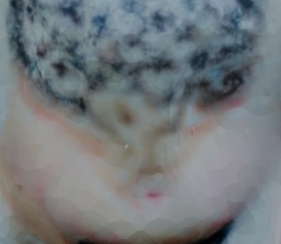
\includegraphics[width=\linewidth]{figures/task1/objectC/firekeeper_wrong_1.png}
			\caption{Mask lacks detail}
		\end{subfigure}
		\hfill
		\begin{subfigure}{0.45\textwidth}
			\centering
			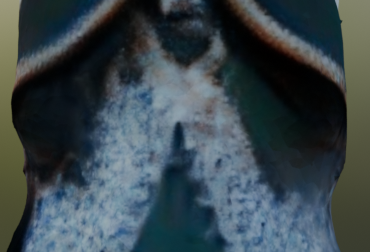
\includegraphics[width=\linewidth]{figures/task1/objectC/firekeeper_wrong_2.png}
			\caption{Hands mistaken as pattern of clothes}
		\end{subfigure}
	\end{minipage}
	\hfill
	% 第二组：Robot
	\begin{minipage}{0.45\textwidth}
		\centering
		\textbf{Robot} \\[1ex]
		\begin{subfigure}{0.45\textwidth}
			\centering
			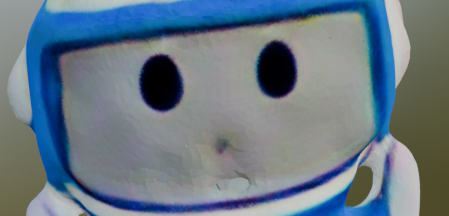
\includegraphics[width=\linewidth]{figures/task1/objectC/robot_wrong_1.png}
			\caption{Poor depth handling}
		\end{subfigure}
		\hfill
		\begin{subfigure}{0.45\textwidth}
			\centering
			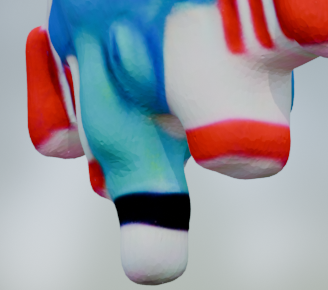
\includegraphics[width=\linewidth]{figures/task1/objectC/robot_wrong_2.png}
			\caption{Joints erased}
		\end{subfigure}
	\end{minipage}
	
	\caption{Failure cases of Object C grouped by subject.}
	\label{fig:objectC_failures}
\end{figure}


\subsection{Fusion Report}

\subsubsection{Fusion Techniques}
Considering that both Object A and Background Scene generate \textbf{point cloud},both Object Bs and Object Cs generate \textbf{mesh}, we export the point cloud as \textbf{gaussian mesh} with the code offered by 2DGS chapter and put all the resources into the Blender.

\subsubsection{Fusion Visualization}
Figure~\ref{fig:Fusion Vis} are some pictures of our fusion results, some include all objects, while some pick one from each category:

\begin{figure}[h]
	\centering
	
	% 第一行：full_1 和 full_2 并排
	\begin{minipage}{0.45\textwidth}
		\centering
		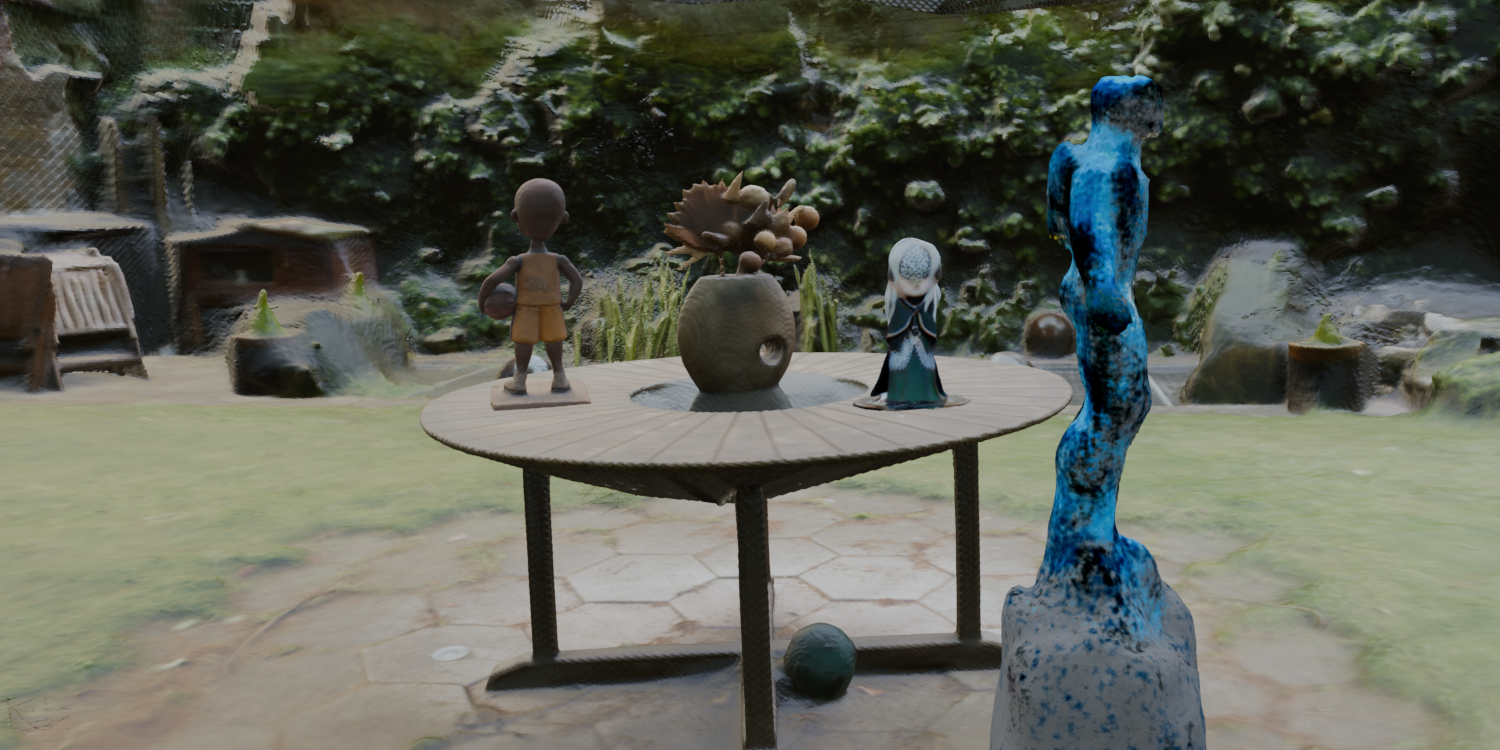
\includegraphics[width=\linewidth]{figures/task1/full_1.png}
	\end{minipage}
	\hfill
	\begin{minipage}{0.45\textwidth}
		\centering
		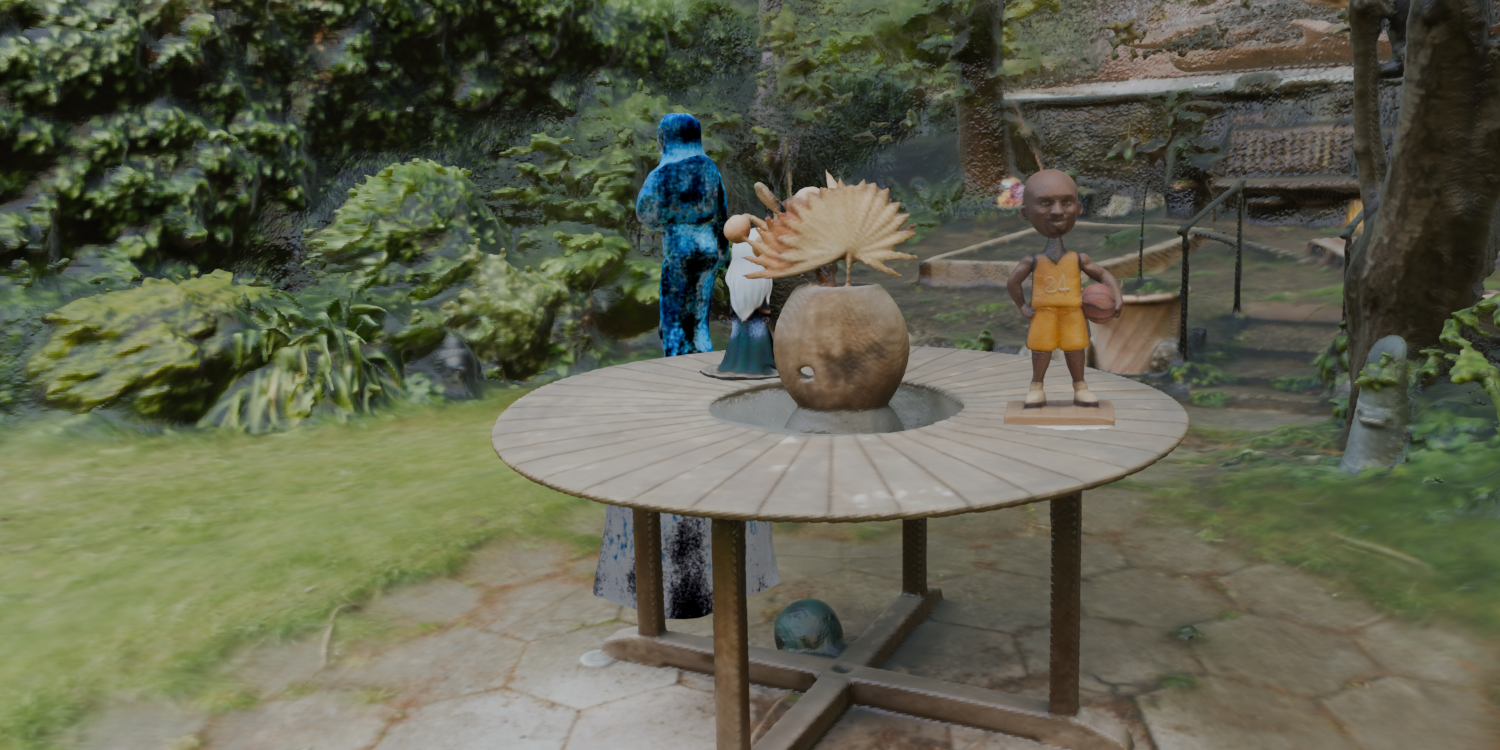
\includegraphics[width=\linewidth]{figures/task1/full_2.png}
	\end{minipage}
	
	\vspace{0.3cm}  % 行间距（可调整）
	
	% 第二行：full_3 和 full_4 并排
	\begin{minipage}{0.45\textwidth}
		\centering
		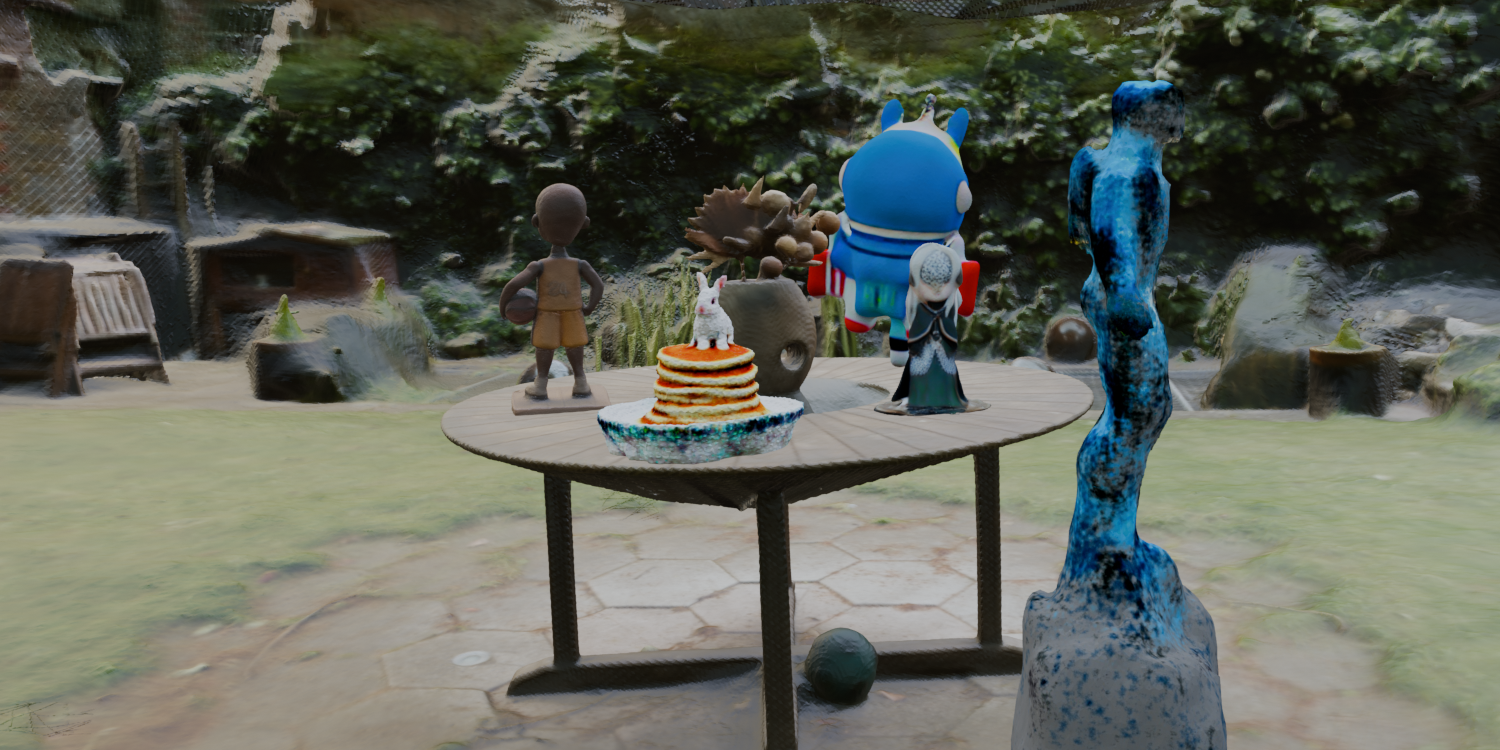
\includegraphics[width=\linewidth]{figures/task1/full_3.png}
	\end{minipage}
	\hfill
	\begin{minipage}{0.45\textwidth}
		\centering
		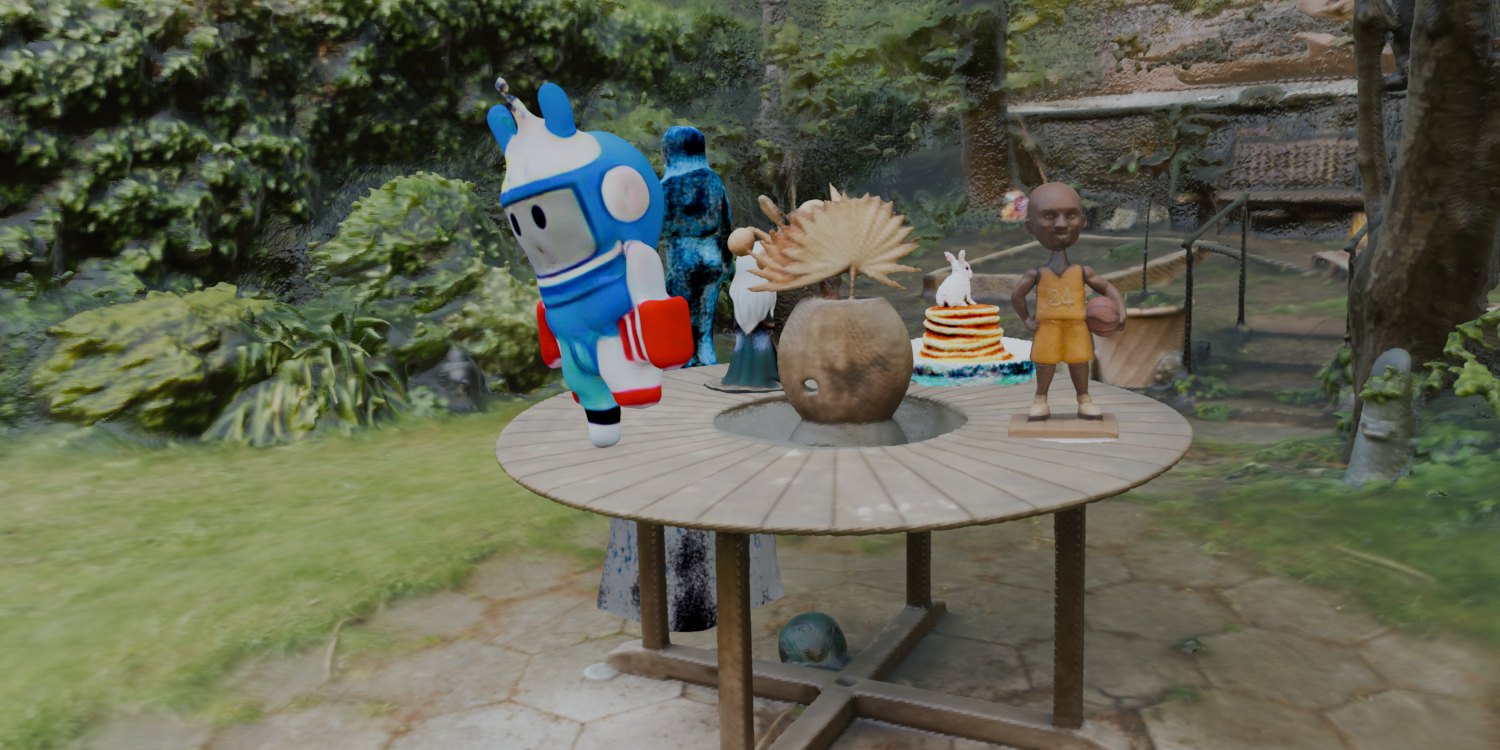
\includegraphics[width=\linewidth]{figures/task1/full_4.png}
	\end{minipage}
	
	\caption{Fusion Visualizations.}
	\label{fig:Fusion Vis}   % 原样保留（包括空格）
\end{figure}

Else, the rendered videos are provided in the appendix (see section~\ref{sec:models}).
\input{sections/task1/Summary.tex}


\section{Task 2: Cross-Environment Generalization of ACT Policies}

Robotic manipulation policies often exhibit strong performance within the environments on which they are trained, yet their performance may degrade significantly when deployed in visually different scenes. Evaluating such cross-environment generalization is therefore an important step toward building robust robot learning systems.

In this task, we investigate the zero-shot transfer capability of Action Chunking with Transformers (ACT) under the visual distribution shifts present in the CALVIN benchmark. Policies are trained using demonstrations collected from one or multiple environments and are subsequently evaluated on the previously unseen Environment D without any additional fine-tuning. We aim to understand whether exposure to a more diverse set of training environments improves robustness to variations in scene appearance, object layouts, and interactive object positions.

To provide a comprehensive assessment, we evaluate policy performance from two complementary perspectives. First, action prediction quality is measured using the Action $L_1$ Error on the full multi-task dataset. Second, practical task execution ability is evaluated through rollout success rates on a task-specific \textit{open drawer} subset in the CALVIN simulator. Together, these experiments provide quantitative evidence regarding the effectiveness of multi-environment training for improving zero-shot cross-environment generalization.

\subsection{Dataset Description}

\subsubsection{Dataset Format}

All experiments were conducted on a processed version of the CALVIN dataset provided by the teaching staff and distributed through Hugging Face. The dataset preserves the original CALVIN environment splits (A, B, C, and D), while the trajectory data are reorganized into a collection of \texttt{.parquet} files for efficient loading and preprocessing.

Each \texttt{.parquet} file corresponds to a complete episode and contains approximately 60 consecutive timesteps. For each timestep, the dataset stores multimodal observations, robot states, expert actions, and auxiliary metadata such as timestamps and episode indices.

In this work, we primarily use the following fields:

\begin{itemize}
    \item \texttt{image}: RGB observation from the static camera.
    \item \texttt{wrist\_image}: RGB observation from the wrist-mounted camera.
    \item \texttt{state}: a 15-dimensional robot state vector.
    \item \texttt{actions}: a 7-dimensional expert action vector.
\end{itemize}

The ACT policy receives both visual observations and robot proprioceptive information as inputs. Specifically, the static camera image, wrist-mounted camera image, and the 15-dimensional state vector are used to represent the current observation of the environment and robot configuration. The 7-dimensional action vector serves as the supervision target during training.

Figure~\ref{fig:data_exploration} shows a visualization of a sample episode from Environment D. The figure includes observations from both cameras, the 15-dimensional state vector at the first frame, and the action trajectory over the first 16 timesteps.

\begin{figure}[h]
    \centering
    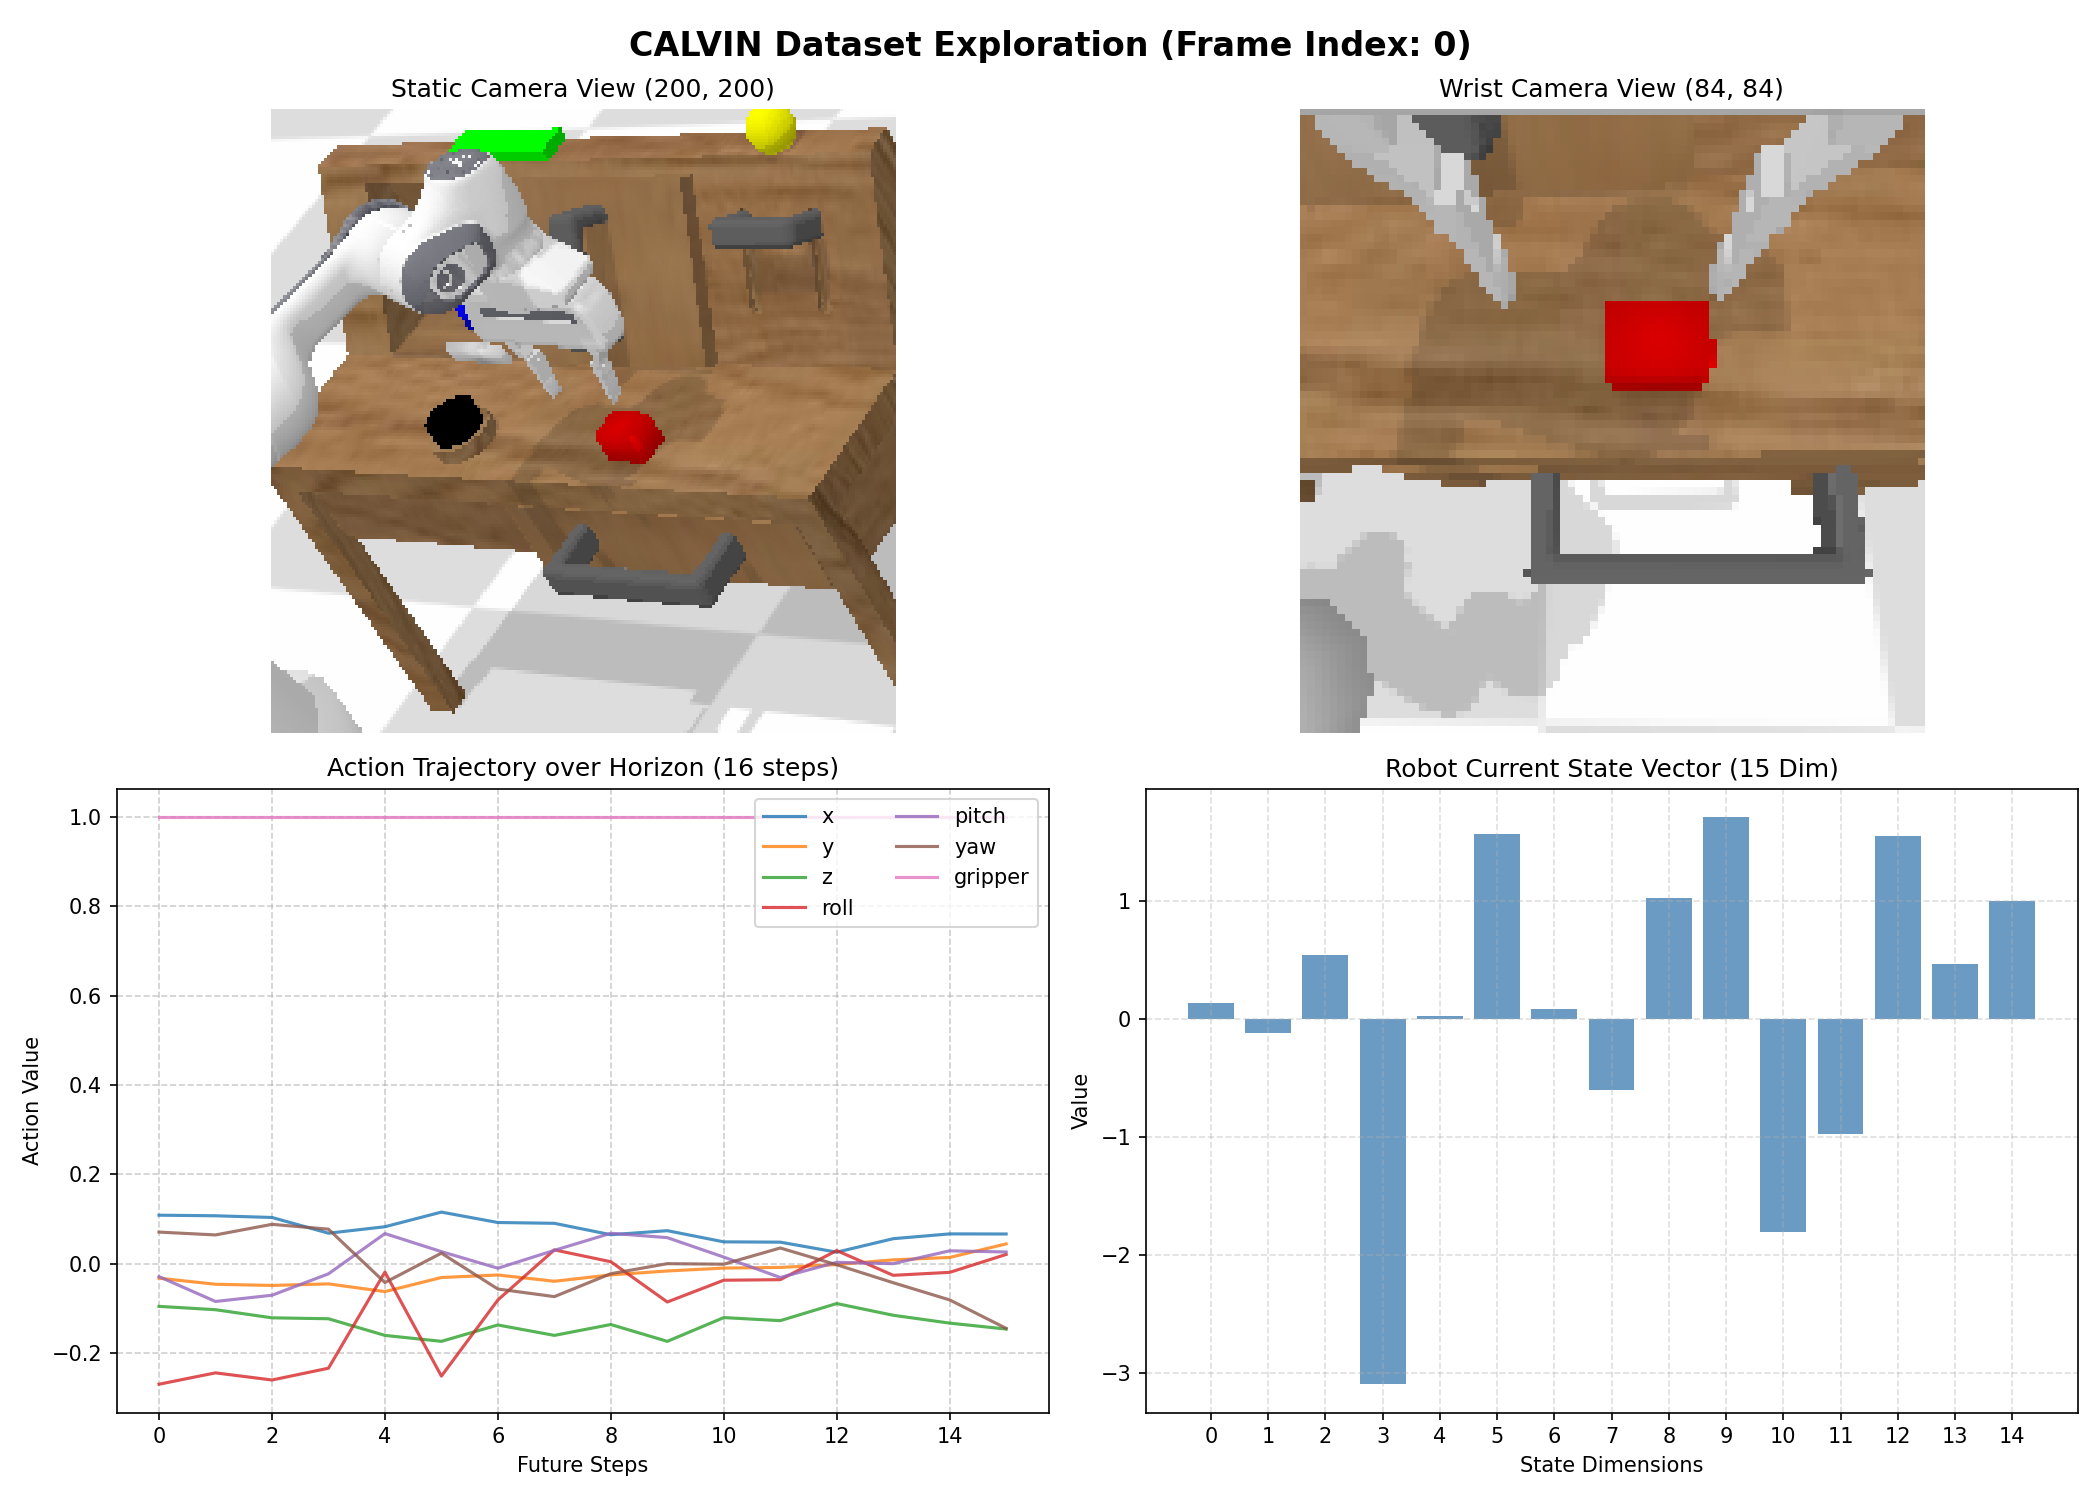
\includegraphics[width=\linewidth]{figures/task2/data_exploration_output_D.png}
    \caption{Visualization of a sample episode from Environment D. The figure shows observations from the static camera and wrist-mounted camera, the 15-dimensional robot state vector at frame 0, and the action trajectory over the first 16 timesteps.}
    \label{fig:data_exploration}
\end{figure}


\subsubsection{Visual Distribution Shift Across Environments}

A central challenge of this project is cross-environment generalization. Although the environments share the same robot platform and a similar set of manipulation tasks, their visual appearances differ substantially.

Figure~\ref{fig:visual_shift} presents representative observations from Environments A, B, C, and D. Differences can be observed in the table textures, object appearances, scene layouts, drawer locations, button positions, and switch placements. These changes create a significant visual distribution shift between training and testing environments.

As a result, a policy trained on one environment may overfit to environment-specific visual features and fail to generalize to unseen scenes. Evaluating policy performance on Environment D therefore provides a practical benchmark for measuring visual robustness and cross-environment transfer capability.

\begin{figure}[h]
    \centering
    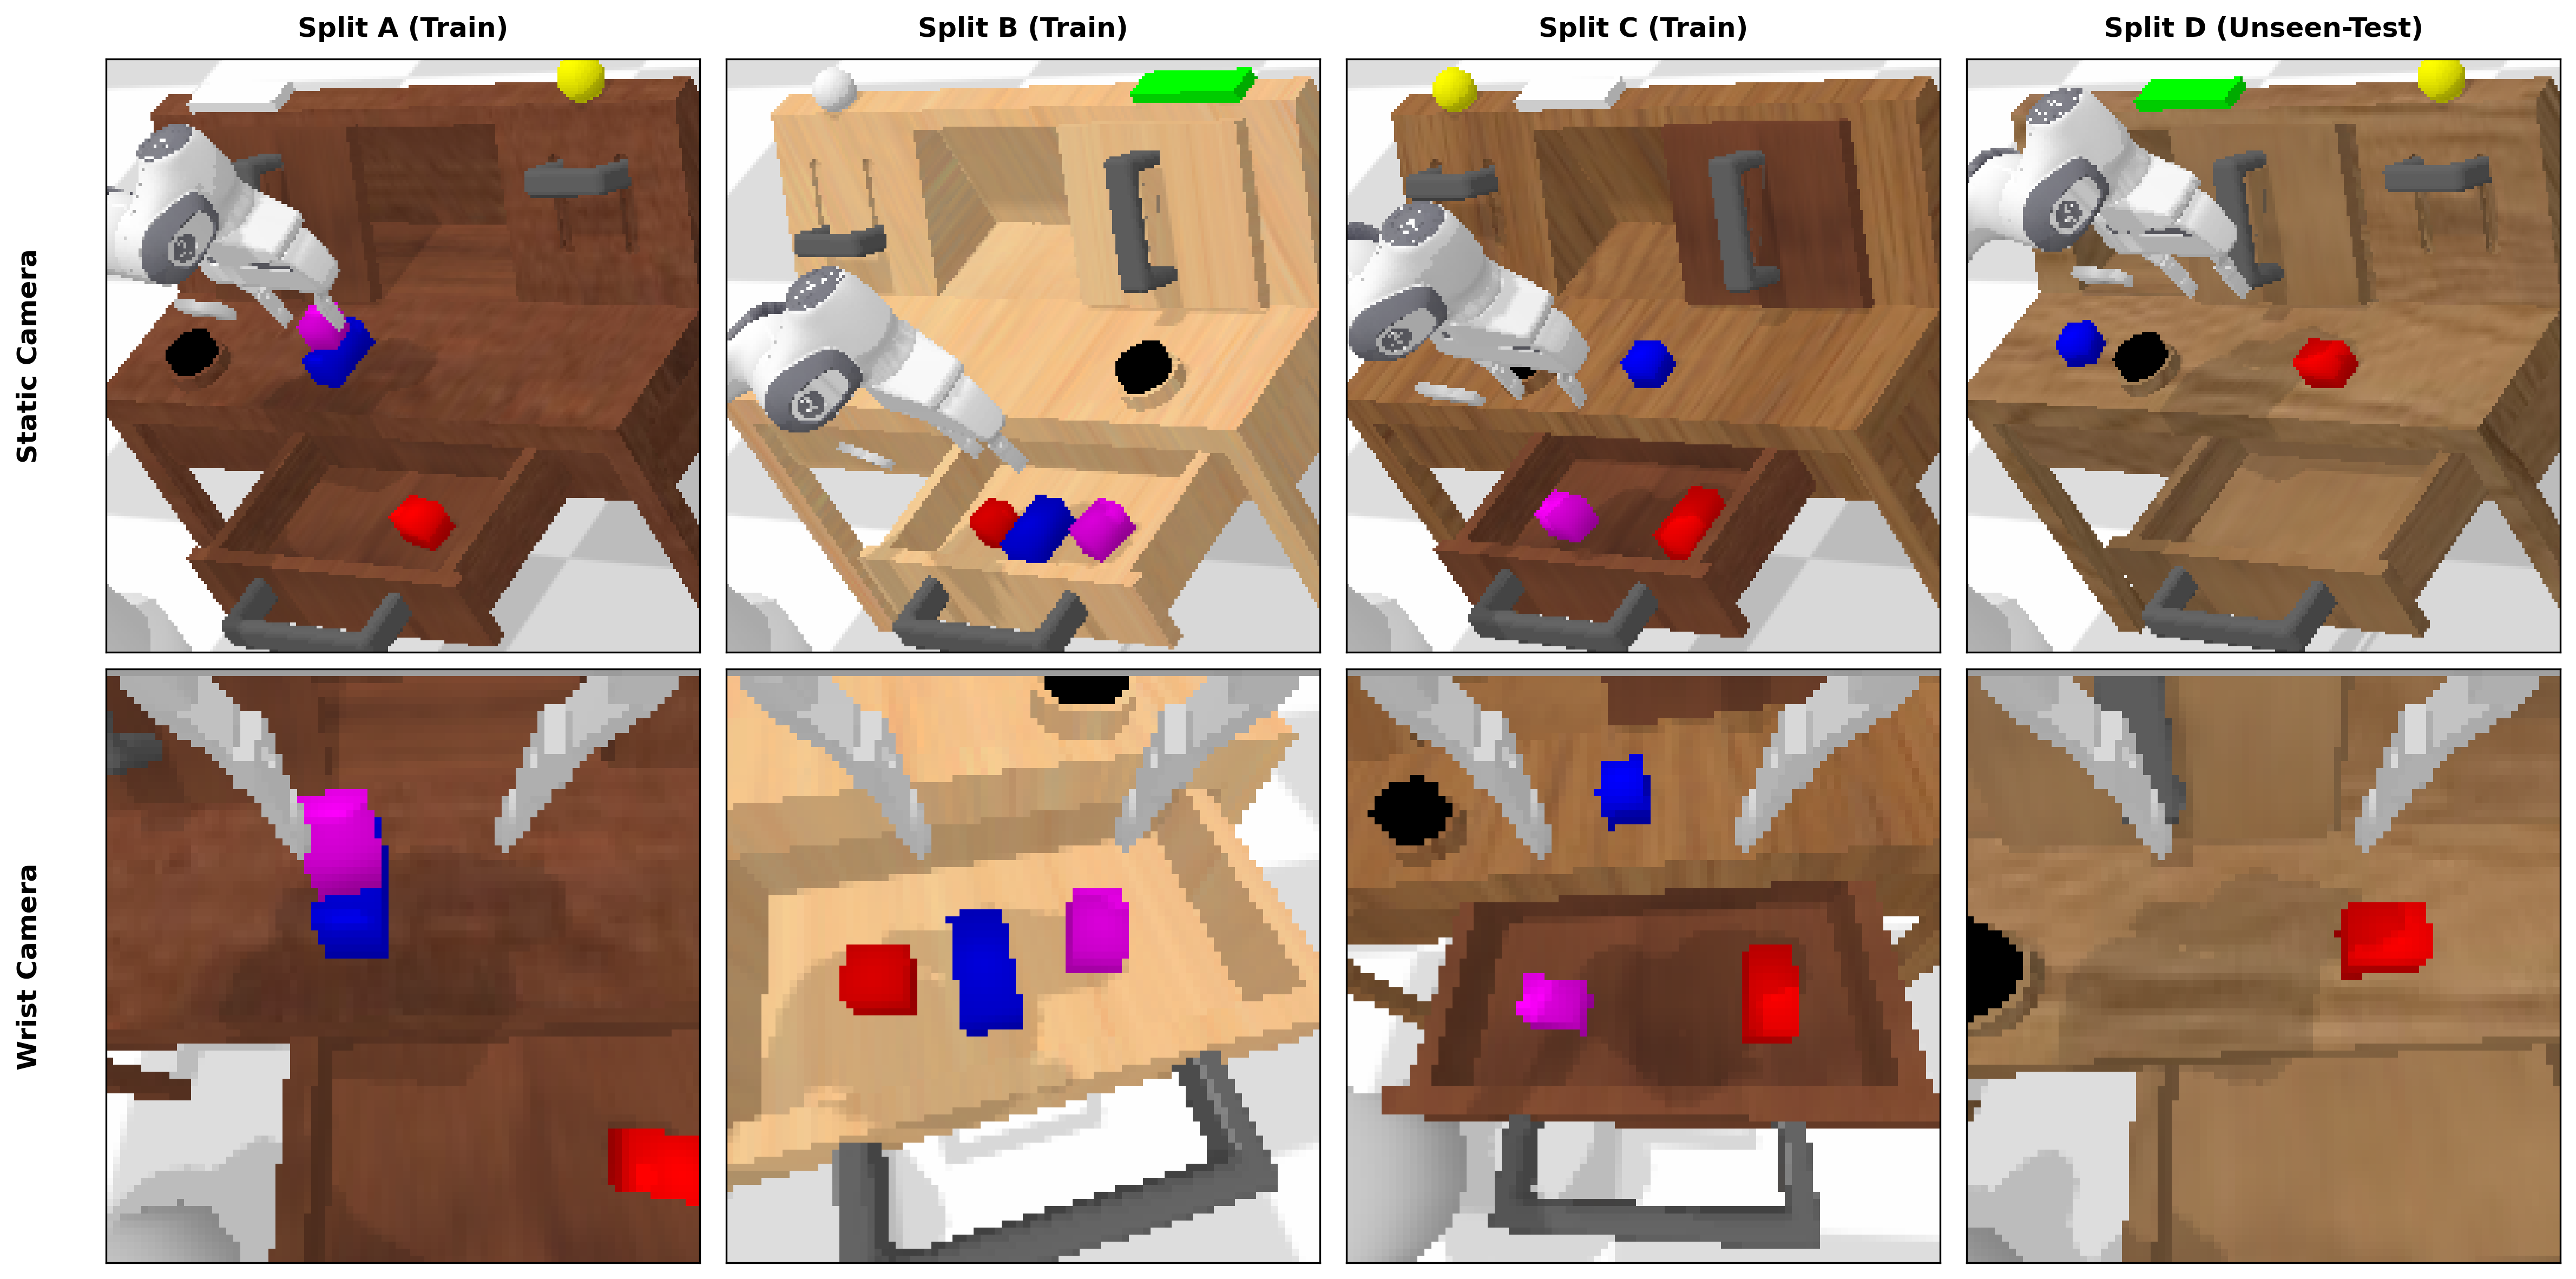
\includegraphics[width=\linewidth]{figures/task2/visual_distribution_shift.png}
    \caption{Representative observations from Environments A, B, C, and D. Variations in scene appearance, object layouts, and interactive object positions introduce substantial visual distribution shifts across environments.}
    \label{fig:visual_shift}
\end{figure}


\subsubsection{Open-Drawer Task Subset}
\label{sec:subset}

Besides the full multi-task dataset, we additionally construct a task-specific subset for success-rate evaluation. Specifically, all trajectories corresponding to the \textit{open drawer} task are extracted from the four environment splits into a filtered dataset.

The motivation for constructing this subset stems from an important difference between our setting and the original CALVIN benchmark. In the original CALVIN framework, policies are conditioned on language instructions that explicitly specify the target task. Consequently, the agent knows which manipulation objective should be executed during rollout.

In contrast, the ACT policy used in this project receives only visual observations and robot state information, without any language input or task identifier. When trained on the full multi-task dataset, the policy observes demonstrations from many different tasks but is not informed which task should be performed at test time. As a result, although action prediction error can still be evaluated offline, task-level success rates become difficult to interpret because the policy lacks explicit task-conditioning information.

To enable meaningful success-rate evaluation, we therefore construct a single-task dataset containing only \textit{open drawer} demonstrations. Under this setting, task ambiguity is removed and the manipulation objective is implicitly specified by the training distribution. This makes it possible to perform rollout-based evaluation and measure task success rate under zero-shot cross-environment transfer.

\subsubsection{Data Preprocessing}

To facilitate ACT training, several preprocessing steps are applied after loading the dataset. The training and validation sets are split at the episode level with a validation ratio of $10\%$ to prevent data leakage between highly correlated frames from the same trajectory. For multi-environment experiments, data from Environments A, B, and C are merged into a unified training set, while Environment D is reserved for zero-shot evaluation.

\subsection{Simulation Environment}

All policy evaluation experiments are conducted in the CALVIN simulation environment. During inference, the trained ACT policy interacts with the simulator in a closed-loop manner: at each timestep, the environment provides visual observations and robot state information, the policy predicts the next action, and the environment executes the action and returns updated observations.

Besides serving as an execution platform, the CALVIN environment provides access to the underlying environment states required for task evaluation. Given a rollout trajectory, these state variables can be used to determine whether a manipulation task has been successfully completed according to predefined task-specific criteria. This functionality enables objective success-rate evaluation and allows quantitative comparison between different policies under zero-shot cross-environment transfer.

\subsection{Method}

\subsubsection{Action Chunking with Transformers}

ACT formulates robot manipulation as a sequence prediction problem. Given the current observations, including visual inputs from the static and wrist cameras as well as the robot state vector, the policy predicts a chunk of future actions instead of only the next action.

Specifically, for an action horizon $H$, the policy outputs a sequence
\[
\mathbf{a}_{t:t+H-1}
=
\left(
\mathbf{a}_t,
\mathbf{a}_{t+1},
\ldots,
\mathbf{a}_{t+H-1}
\right),
\]
where each action consists of three translational components, three rotational components, and one gripper control signal.

Following the original ACT architecture, visual features extracted from the camera observations and proprioceptive robot states are fused and processed by a Transformer-based policy network. Predicting multiple future actions jointly encourages the model to capture longer temporal dependencies and produces smoother action sequences. Action chunking can also improve robustness against visual distribution shifts, and the influence of different horizon lengths is further investigated in the ablation study.

Following the original ACT architecture, visual features extracted from the camera observations and proprioceptive robot states are fused and processed by a Transformer-based policy network. Predicting multiple future actions jointly encourages the model to capture longer temporal dependencies and produces smoother action sequences. Action chunking can also improve robustness against visual distribution shifts, and the influence of different horizon lengths is further investigated in the ablation study.

The training objective consists of an action reconstruction term and a latent regularization term:
\[
\mathcal{L}
=
\mathcal{L}_{\text{action}}
+
\beta \mathcal{L}_{\text{KL}},
\]
where $\mathcal{L}_{\text{action}}$ measures the discrepancy between predicted and expert actions, $\mathcal{L}_{\text{KL}}$ is the Kullback--Leibler divergence term introduced by the conditional VAE formulation, and $\beta$ denotes the KL weight.

During inference, the policy predicts an action chunk at every timestep. Unless otherwise specified, the first predicted action in the chunk is executed:
\[
\hat{\mathbf a}_t
=
\left(\hat{\mathbf a}_{t:t+H-1}\right)_0.
\]

\begin{figure}[h]
    \centering
    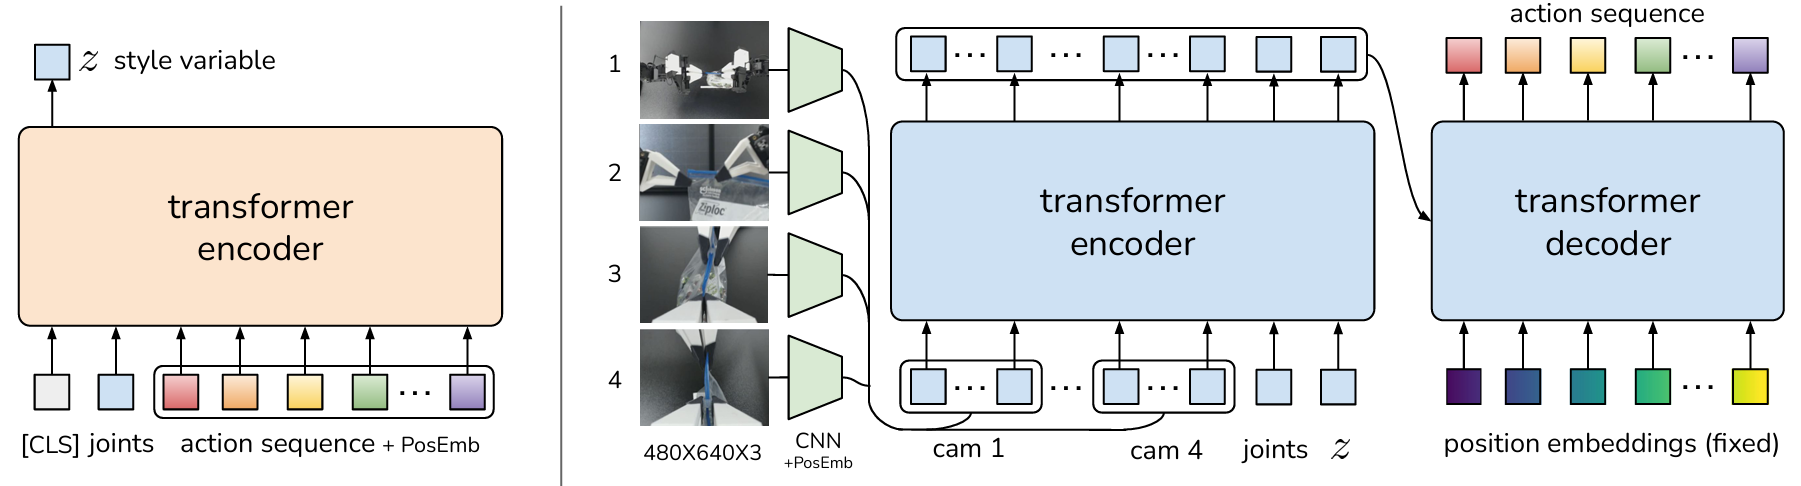
\includegraphics[width=0.95\linewidth]{figures/task2/ACT.png}
    \caption{Overview of the ACT architecture. Given visual observations and robot states, the policy predicts a chunk of future actions using a Transformer-based sequence model.}
    \label{fig:act_architecture}
\end{figure}

\subsubsection{Training Strategy}

We adopt the ACT implementation provided by the LeRobot framework. The policy receives observations from the static camera, wrist camera, and robot state vector, and predicts future action chunks in an end-to-end manner.

Two training settings are considered. The first uses only Environment B for training, corresponding to a single-environment policy. The second combines data from Environments A, B, and C into a unified training set while keeping the network architecture and hyperparameters unchanged. This setting exposes the policy to a broader range of visual appearances and object configurations during training.

Both settings are evaluated on two datasets. The first is the full multi-task CALVIN dataset, which is used to analyze action prediction performance under cross-environment transfer. The second is the task-specific \textit{open drawer} subset introduced in Section~\ref{sec:subset}, which enables closed-loop success-rate evaluation in the simulation environment.

For all experiments, model selection is performed using a validation set sampled from the corresponding training environments. The checkpoint with the best validation performance is retained and subsequently evaluated on the unseen Environment D to assess zero-shot cross-environment generalization.

\subsection{Experimental Setup}

\subsubsection{Training Configurations}

All experiments share a common set of network and optimization hyperparameters unless explicitly stated otherwise. Some later ablation studies modify specific settings, such as the action horizon, to investigate their influence on policy performance.

\begin{table}[h]
\centering
\caption{Default training hyperparameters.}
\label{tab:training_config}
\begin{tabular}{lc}
\toprule
Parameter & Value \\
\midrule
Visual Backbone & ResNet-18 \\
Transformer Hidden Dimension & 512 \\
Feedforward Dimension & 3200 \\
KL Weight & 5 \\
Batch Size & 64 \\
Action Horizon & 4 \\
Optimizer & AdamW \\
Transformer Learning Rate & $1\times10^{-4}$ \\
Backbone Learning Rate & $1\times10^{-5}$ \\
Weight Decay & $1\times10^{-4}$ \\
Learning Rate Scheduler & Cosine Annealing \\
Validation Split Ratio & 10\% \\
Random Seed & 42 \\
\bottomrule
\end{tabular}
\end{table}

Two types of datasets are considered in this work. The full CALVIN dataset is used for action prediction experiments under zero-shot cross-environment transfer, while the filtered \textit{open drawer} subset is used for success-rate evaluation in closed-loop simulation.

\begin{table}[h]
\centering
\caption{Main experimental settings.}
\label{tab:experiment_settings}
\begin{tabular}{lcc}
\toprule
Setting & Training Environments & Epochs \\
\midrule
B & B & 3 \\
ABC & A+B+C & 1 \\
Filtered-B & B (\textit{open drawer}) & 60 \\
Filtered-ABC & A+B+C (\textit{open drawer}) & 20 \\
\bottomrule
\end{tabular}
\end{table}

For the full-dataset experiments, Environment B contains approximately one-third of the training samples available in the combined A+B+C dataset. Therefore, the B and ABC settings use 3 and 1 training epochs, respectively, resulting in a comparable number of optimization steps and ensuring a fair comparison between single-environment and multi-environment training.

For the \textit{open drawer} subset, the amount of available training data is substantially smaller. Consequently, longer training schedules (60 and 20 epochs, respectively) are adopted to ensure sufficient convergence while maintaining a similar ratio of optimization steps between the single-environment and multi-environment settings.

For all experiments, model selection is performed using the validation split from the corresponding training environments. The checkpoint achieving the best validation performance is retained for subsequent evaluation on the unseen Environment D.

\subsubsection{Evaluation Metrics}

Two complementary metrics are adopted to evaluate cross-environment generalization.

\paragraph{Action L1 Error.}
For a predicted action sequence $\hat{\mathbf{a}}$ and the corresponding expert action sequence $\mathbf{a}$, the action prediction error is measured using the average L1 distance

\[
\frac{1}{N}
\sum_{i=1}^{N}
\left|
\hat{\mathbf{a}}_i-\mathbf{a}_i
\right|,
\]

where $N$ denotes the total number of action dimensions across all evaluated timesteps. Lower values indicate better agreement with expert demonstrations. This metric is computed on the held-out Environment D and serves as the primary evaluation criterion for the full multi-task experiments.

\paragraph{Success Rate.}
For the task-specific \textit{open drawer} subset, policy performance is additionally evaluated through closed-loop rollouts in the CALVIN simulator. A rollout is considered successful if the drawer reaches the predefined completion condition within the maximum allowed horizon. Success rate is defined as

\[
\frac{\#\text{Successful Rollouts}}
{\#\text{Total Rollouts}}
\times 100\%.
\]

Compared with action prediction error, success rate directly measures whether the predicted actions can accomplish the intended manipulation task and therefore provides a more practical assessment of policy generalization.


\subsection{Zero-Shot Generalization: Action Prediction Analysis}

This experiment investigates whether multi-environment training can improve the zero-shot generalization capability of ACT under visual distribution shifts. We compare a model trained solely on Environment B with a model trained jointly on Environments A, B, and C. Both models are evaluated on the unseen Environment D using the action prediction metric introduced previously.

\subsubsection{Training Dynamics}

Figure~\ref{fig:full_training_curves} shows the training and validation curves of the two training strategies. For clarity, the vertical axes of the training-loss plots are cropped at $0.5$, since the losses at the beginning of training are substantially larger and would otherwise obscure the later-stage behavior.

The single-environment model consistently achieves a slightly lower training action reconstruction loss than the multi-environment model. This behavior is expected because the B-only setting involves a narrower visual distribution and therefore constitutes an easier learning problem. In contrast, the ABC model must simultaneously fit demonstrations collected from three visually distinct environments.

The KL-divergence curves of the two models almost completely overlap throughout training, indicating that the latent regularization term is largely unaffected by the choice of training environments. Consequently, the difference in total loss is primarily caused by the action reconstruction term.

Interestingly, the validation action error exhibits a different trend. Although the difference is relatively small, the ABC model achieves slightly lower validation error than the B-only model. Since the validation sets are sampled from the same distributions as the corresponding training sets, this observation alone does not demonstrate cross-environment generalization. Nevertheless, it suggests that exposure to multiple environments may improve the robustness of the learned policy.

\begin{figure}[h]
\centering
\begin{subfigure}{0.48\linewidth}
    \centering
    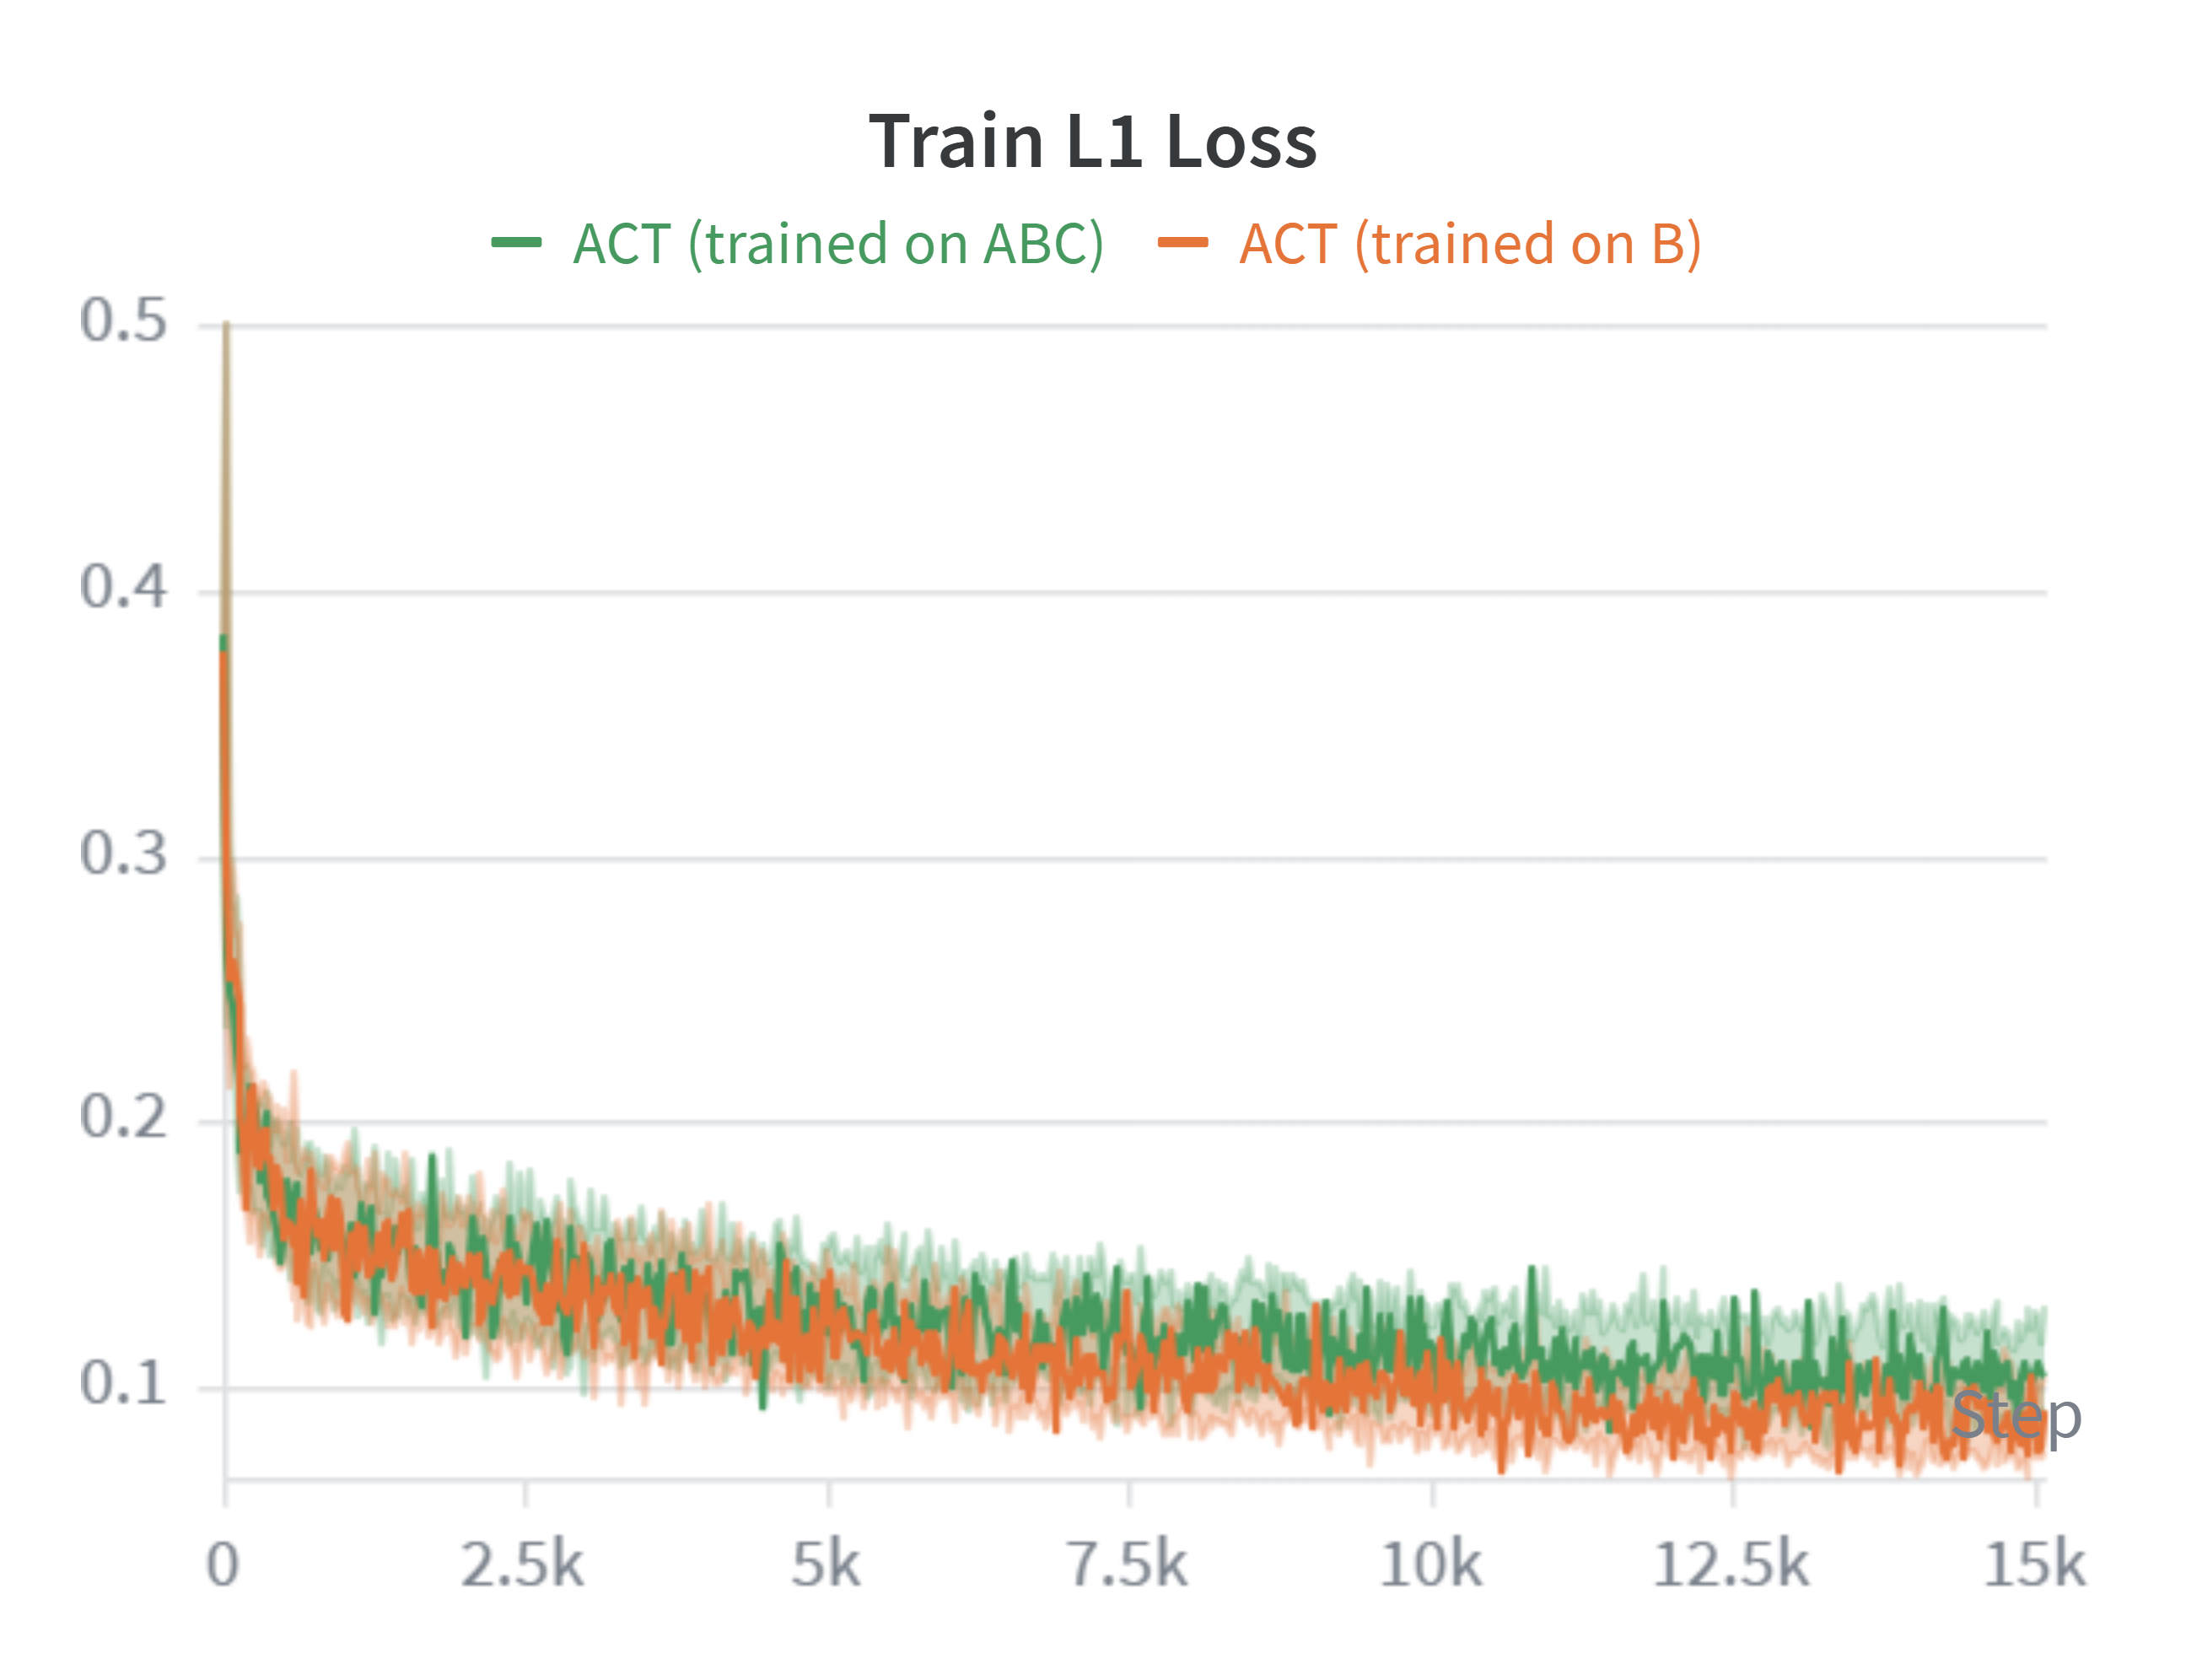
\includegraphics[width=\linewidth]{figures/task2/full_data_train_l1_loss.png}
    \caption{Training Action Loss}
\end{subfigure}
\hfill
\begin{subfigure}{0.48\linewidth}
    \centering
    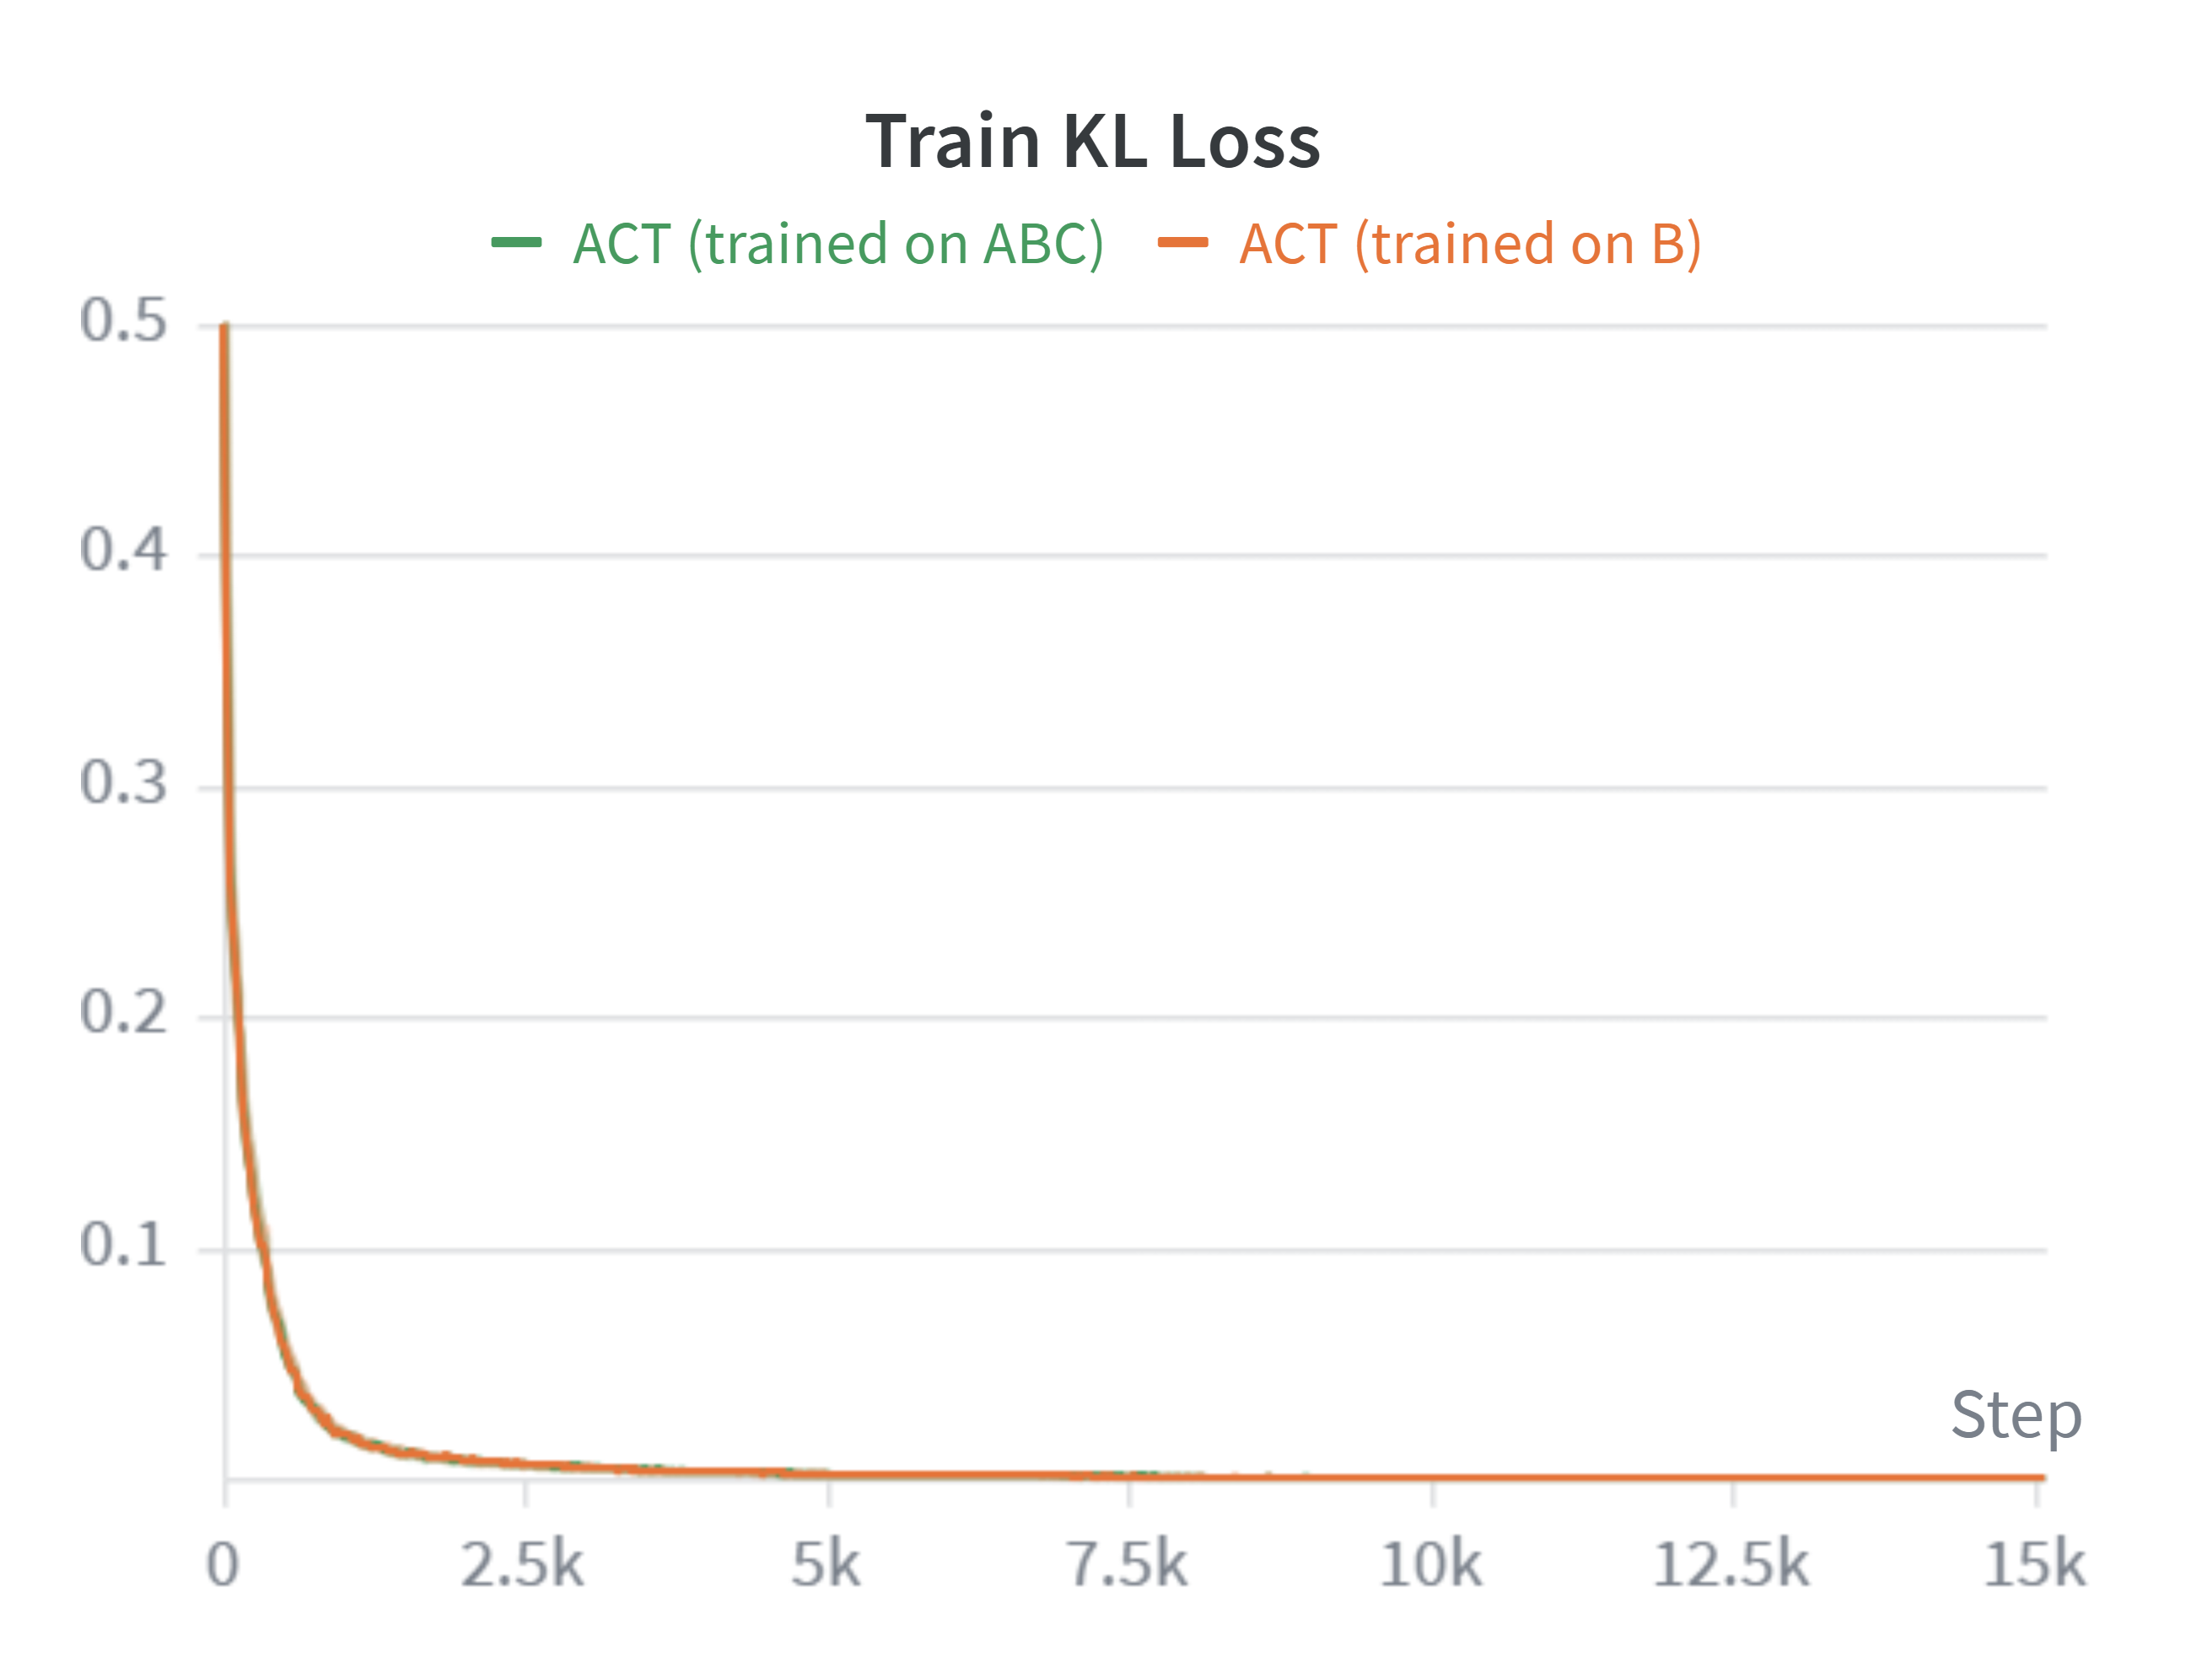
\includegraphics[width=\linewidth]{figures/task2/full_data_train_kl_loss.png}
    \caption{Training KL Loss}
\end{subfigure}

\vspace{0.5em}

\begin{subfigure}{0.48\linewidth}
    \centering
    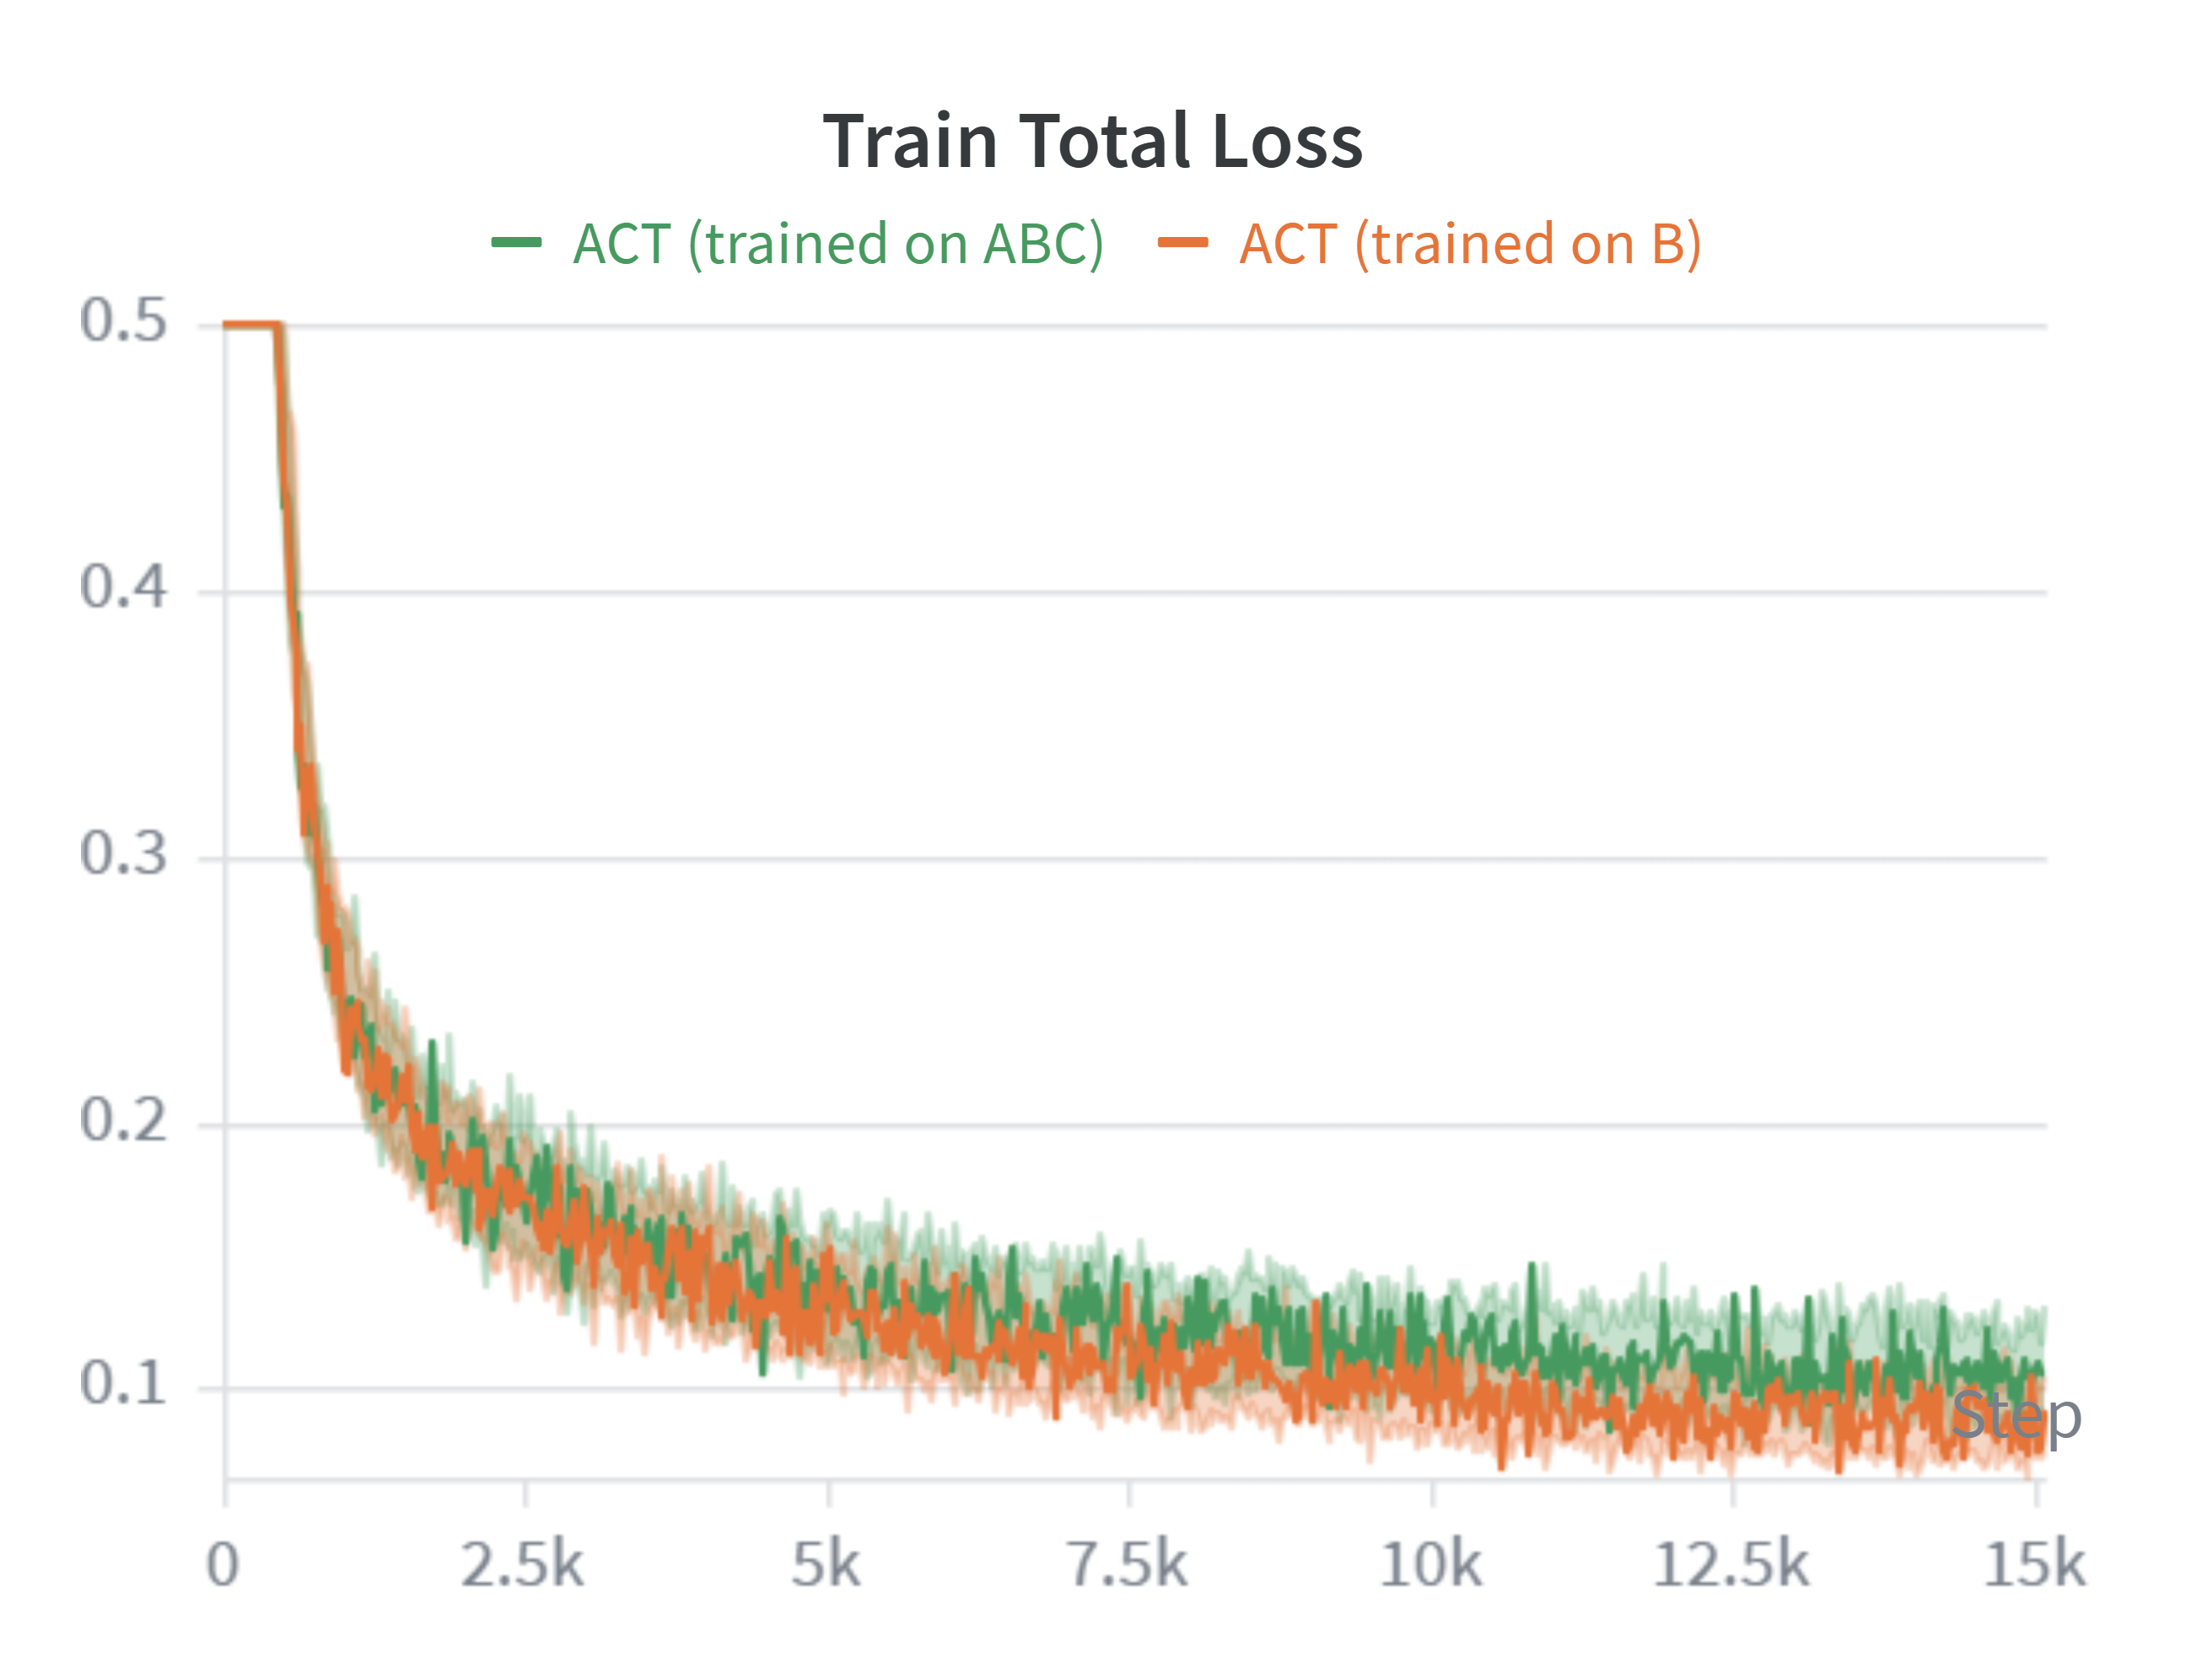
\includegraphics[width=\linewidth]{figures/task2/full_data_train_total_loss.png}
    \caption{Training Total Loss}
\end{subfigure}
\hfill
\begin{subfigure}{0.48\linewidth}
    \centering
    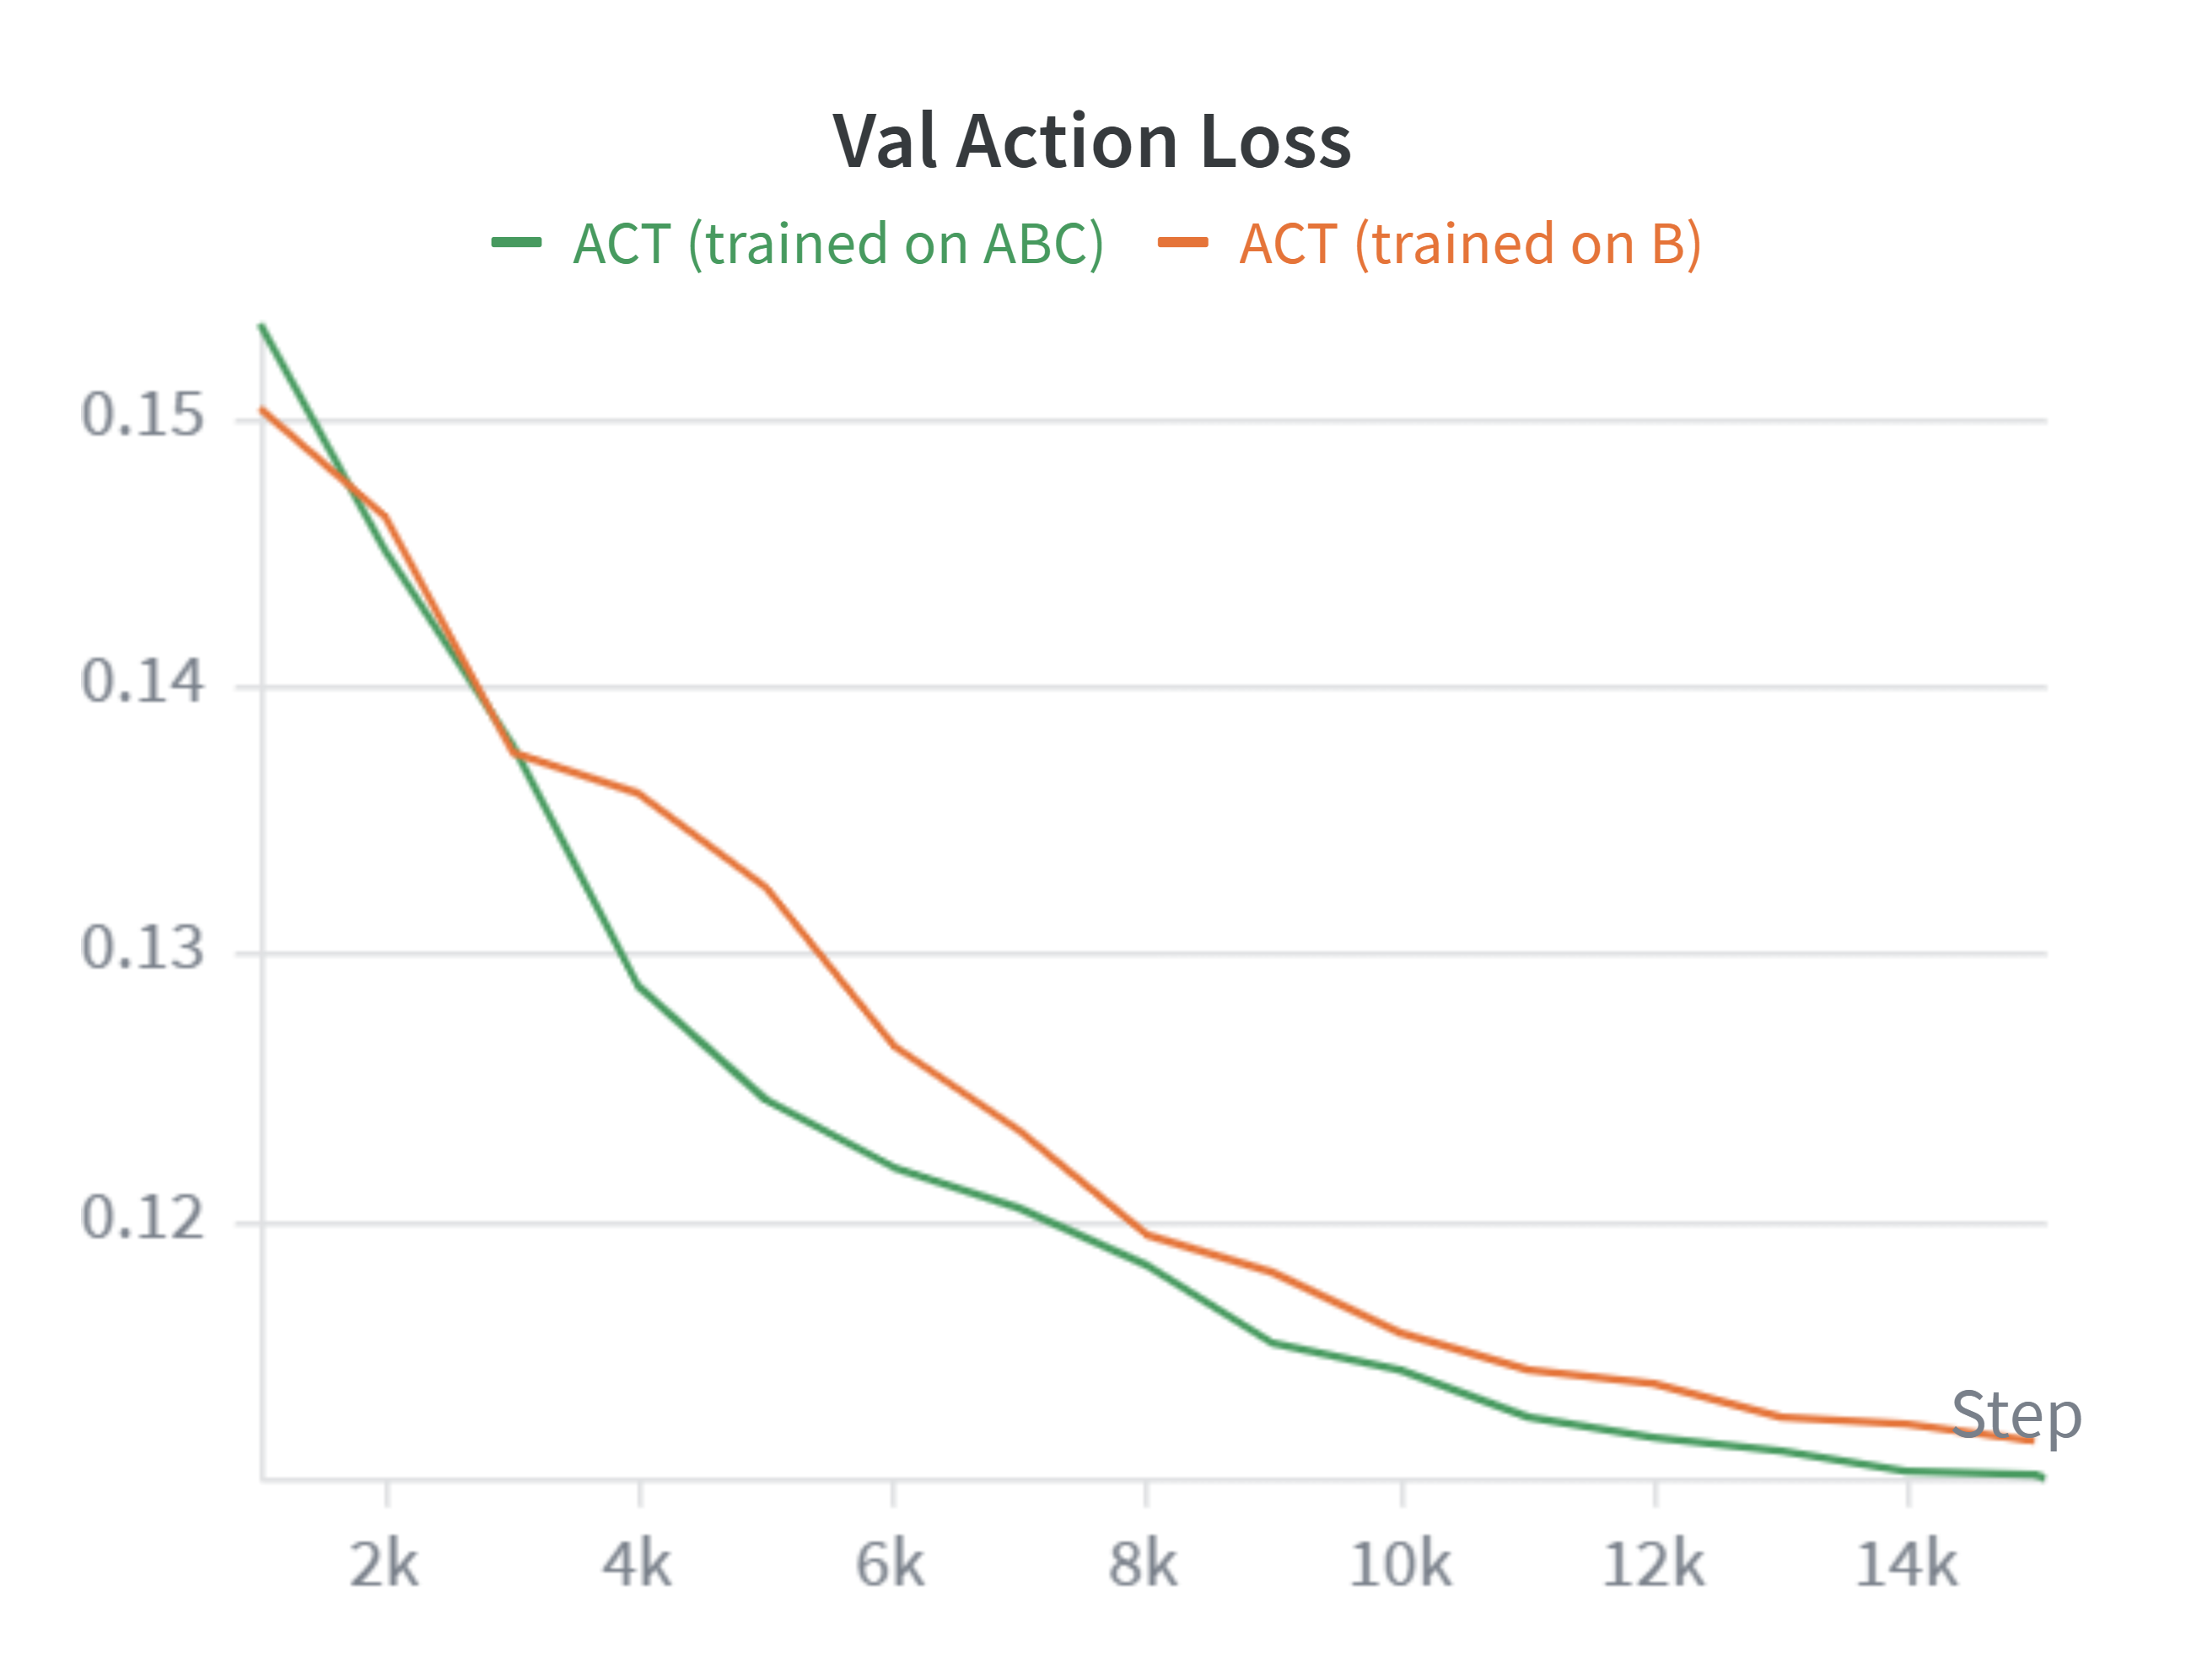
\includegraphics[width=\linewidth]{figures/task2/full_data_val_action_loss.png}
    \caption{Validation Action Error}
\end{subfigure}

\caption{Training and validation curves for the B-only and ABC models. The vertical axes of the three training-loss plots are cropped at $0.5$ for better visualization of the convergence behavior.}
\label{fig:full_training_curves}

\end{figure}

\subsubsection{Zero-Shot Evaluation on Environment D}

The ultimate objective of this task is zero-shot transfer to an unseen environment. Therefore, both models are evaluated on Environment D without any additional fine-tuning.

To ensure a fair comparison, the total number of optimization steps is approximately matched between the two settings. Since the ABC dataset contains roughly three times as many training samples as Environment B alone, the B-only model is trained for 3 epochs while the ABC model is trained for 1 epoch. We additionally conduct a longer-training experiment using 9 epochs for B and 3 epochs for ABC.

\begin{table}[h]
\centering
\caption{Zero-shot action prediction error on Environment D.}
\label{tab:zero_shot_results}
\begin{tabular}{lcc}
\toprule
Training Environments & Epochs & Action L1 Error \\
\midrule
B & 3 & 0.14339 \\
A+B+C & 1 & \textbf{0.12084} \\
\midrule
B & 9 & 0.17009 \\
A+B+C & 3 & \textbf{0.12039} \\
\bottomrule
\end{tabular}
\end{table}

The results reveal a substantial advantage of multi-environment training. Despite achieving a slightly higher training loss, the ABC model consistently outperforms the B-only model on the unseen Environment D.

Under approximately matched optimization budgets, the action error decreases from $0.14339$ to $0.12084$, corresponding to a relative improvement of approximately $15.7\%$. The same trend persists in the longer-training setting, where the ABC model reaches an error of $0.12039$, whereas the B-only model deteriorates to $0.17009$.

A particularly interesting observation is that extending the training duration further reduces the validation loss in both settings, yet yields little or no improvement in zero-shot performance. While the ABC model remains essentially unchanged, the performance of the B-only model deteriorates noticeably. This behavior suggests that prolonged training may lead to overfitting to environment-specific visual characteristics, especially when only a single training environment is available.

Overall, the results support two conclusions. First, training on multiple environments leads to substantially more robust cross-environment performance than training on a single environment. Second, simply increasing the amount of training provides limited benefits for zero-shot transfer and may even be detrimental due to overfitting. Therefore, improving the diversity of training environments appears to be a more effective strategy than extending training duration when the goal is cross-environment generalization.

\subsubsection{Dimension-wise Error Analysis}

To better understand the source of the performance gain, we further analyze the prediction error of each action dimension using the B (3 epochs) and ABC (1 epoch) models.

\begin{table}[h]
\centering
\caption{Dimension-wise action prediction error on Environment D.}
\label{tab:dimension_error}
\begin{tabular}{lcc}
\toprule
Dimension & B & A+B+C \\
\midrule
X (Translation) & 0.17648 & \textbf{0.14822} \\
Y (Translation) & 0.14265 & \textbf{0.11757} \\
Z (Translation) & 0.16361 & \textbf{0.12844} \\
Roll & 0.11668 & \textbf{0.10879} \\
Pitch & 0.13542 & \textbf{0.11471} \\
Yaw & 0.21472 & \textbf{0.17690} \\
Gripper & 0.05418 & \textbf{0.05127} \\
\bottomrule
\end{tabular}
\end{table}

The improvement is observed consistently across all seven action dimensions. The largest gains occur in the translational coordinates and the yaw rotation component, which are also the dimensions exhibiting the highest errors overall.

This observation is consistent with the nature of visual distribution shifts in CALVIN. Variations in object appearance, texture, and scene layout primarily affect the robot's spatial perception of the environment. Consequently, Cartesian positioning and orientation estimation are more sensitive to environment changes than gripper control.

Figure~\ref{fig:dimension_analysis} visualizes the predicted actions and the corresponding action errors on a representative trajectory from Environment D. Although noticeable discrepancies remain, the predicted trajectories generally capture the overall trends of the expert actions. In contrast, the gripper dimension exhibits substantially lower errors than the motion-related dimensions. A possible explanation is that gripper actions are often easier to infer from the current visual observation. For example, the policy may predict a closing action after observing that the gripper is already in a closed state, rather than anticipating the closing action beforehand. This interpretation is supported by the observation that the predicted gripper signals appear to lag slightly behind the expert actions in some segments.

\begin{figure}[h]
\centering
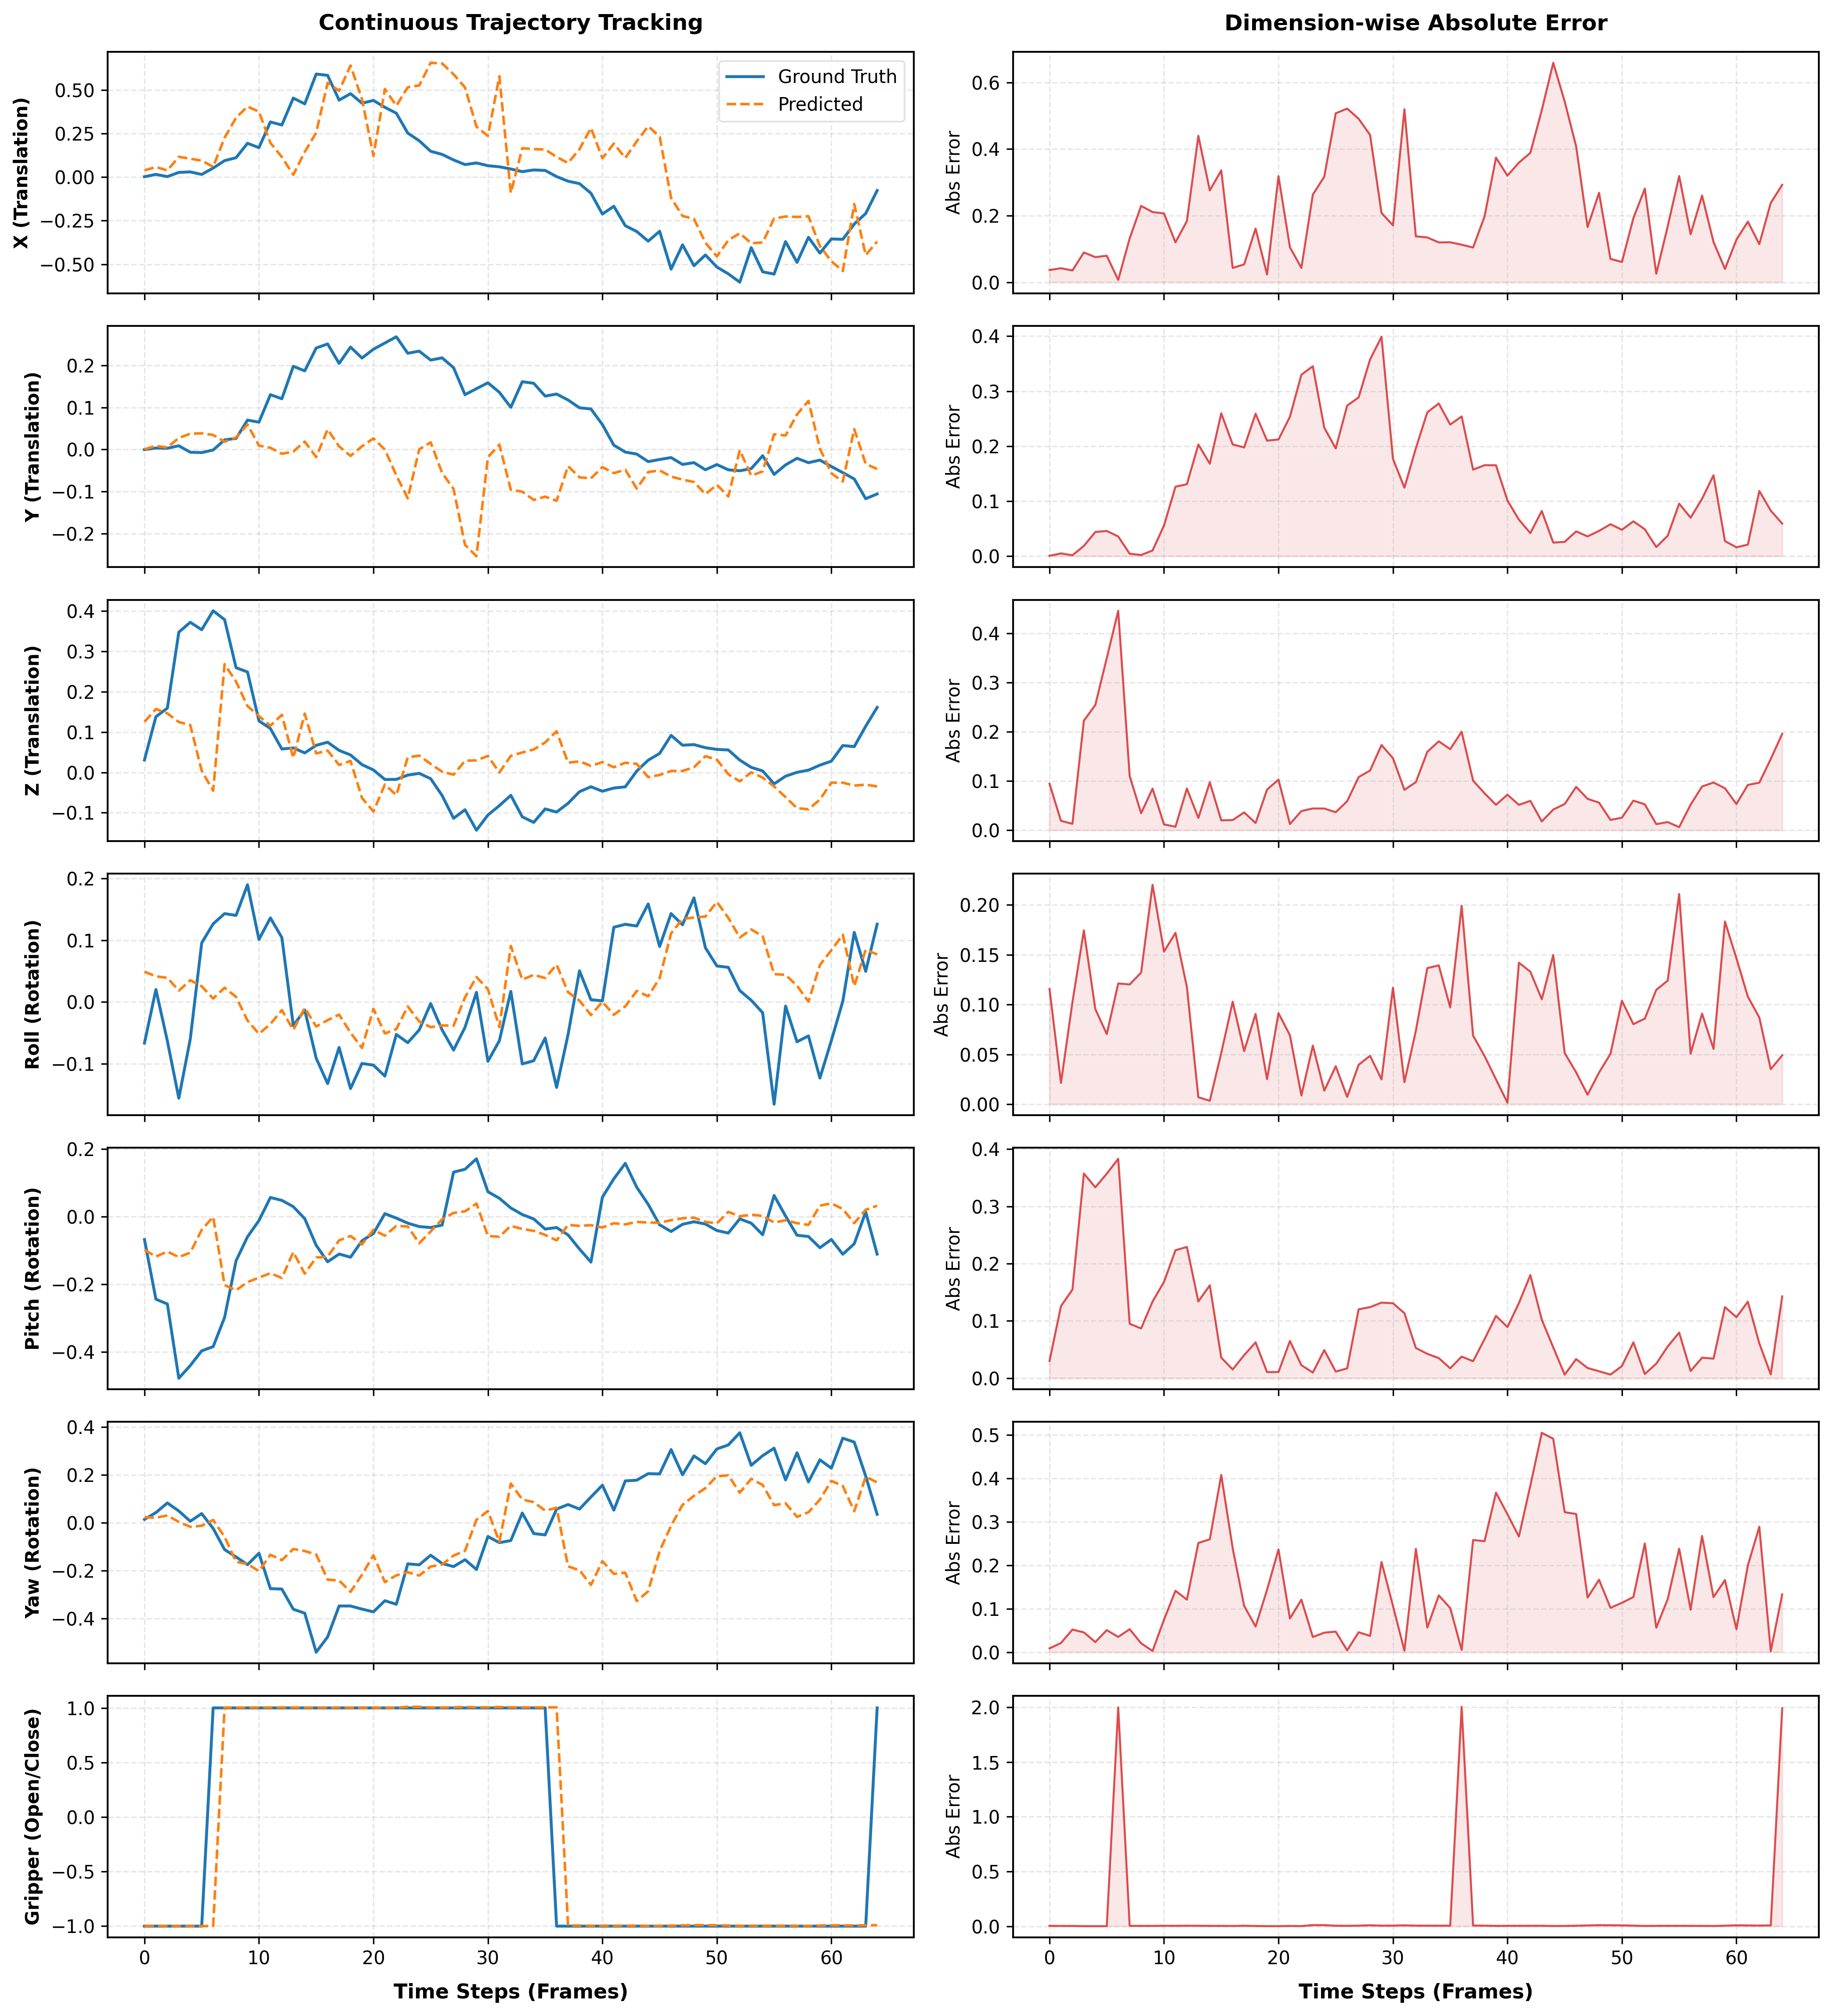
\includegraphics[width=\linewidth]{figures/task2/splitD_episode_000001_dim_analysis.png}
\caption{Dimension-wise prediction analysis on a representative trajectory from Environment D. For each action dimension, the figure shows the expert trajectory, predicted trajectory, and the corresponding absolute prediction error.}
\label{fig:dimension_analysis}
\end{figure}

\subsection{Zero-Shot Generalization: Task Success Rate Analysis}

The previous experiments demonstrated that multi-environment training improves action prediction accuracy under visual distribution shifts. However, action-level metrics do not directly reflect whether a manipulation task can be completed successfully. Therefore, we further evaluate the trained policies on the task-specific \textit{open drawer} subset using closed-loop rollouts in Environment D.

For this experiment, the policies are trained on the filtered \textit{open drawer} dataset described in Section~\ref{sec:subset}. The B-only model is trained for 60 epochs, while the ABC model is trained for 20 epochs. Both models achieve relatively low action prediction errors on the unseen Environment D (0.10769 and 0.09346 respectively), suggesting that the action-level gap between the two policies is modest.

\subsubsection{Success Rate Evaluation}

The success-rate results, however, reveal a dramatically different picture. Over 200 evaluation rollouts in Environment D, the B-only policy fails in every trial, yielding a success rate of $0\%$. In contrast, the ABC policy successfully completes all 200 rollouts, achieving a success rate of $100\%$.

\begin{table}[h]
\centering
\caption{Open-drawer success-rate evaluation in Environment D.}
\label{tab:open_drawer_success}
\begin{tabular}{lcc}
\toprule
Training Setting & Success Rollouts & Success Rate \\
\midrule
Filtered-B & 0 / 200 & 0.0\% \\
Filtered-ABC & 200 / 200 & 100.0\% \\
\bottomrule
\end{tabular}
\end{table}

Interestingly, the difference in task success is far more pronounced than the corresponding difference in action prediction error. The average action error decreases by only about $13.2\%$ (0.10769 $\rightarrow$ 0.09346), yet the success rate improves from $0\%$ to $100\%$. This result highlights a key characteristic of robotic manipulation tasks: small action errors can accumulate over time and eventually lead to task failure when precise physical interactions are required. Consequently, success rate provides a more meaningful evaluation metric than action prediction error alone for assessing practical task performance.

\subsubsection{Analysis of Success and Failure Cases}

To better understand the failure modes, Figure~\ref{fig:open_drawer_success_failure} compares representative successful and failed rollouts. In both cases, the robot initially moves toward the drawer handle, indicating that the high-level task objective has been learned. The critical difference emerges during the grasping phase. In the failed rollout, the gripper stops slightly outside the handle opening and therefore cannot establish a stable grasp. As the arm subsequently moves away from the table, the drawer remains closed. In contrast, the successful rollout positions the gripper inside the handle before executing the pulling motion, allowing the drawer to be opened successfully.

\begin{figure}[h]
    \centering
    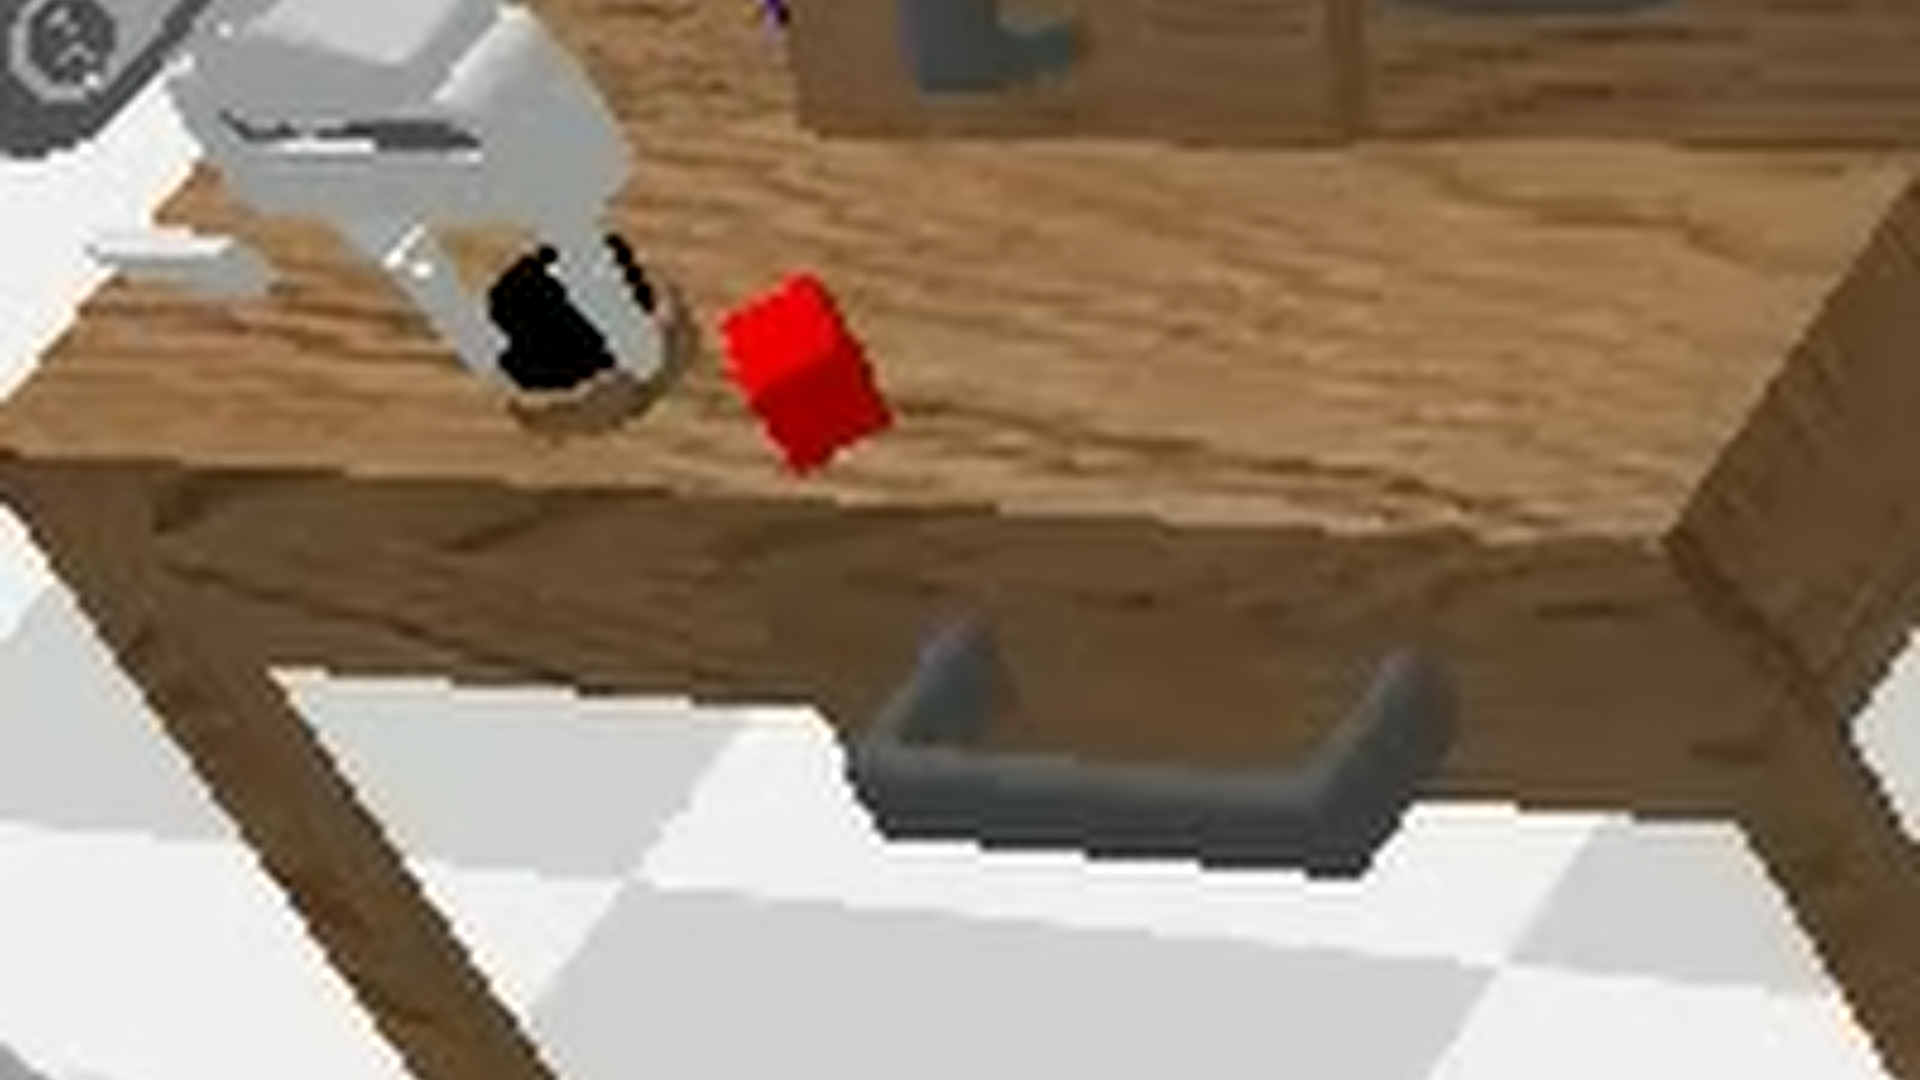
\includegraphics[width=0.24\linewidth]{figures/task2/fail_0.jpg}
    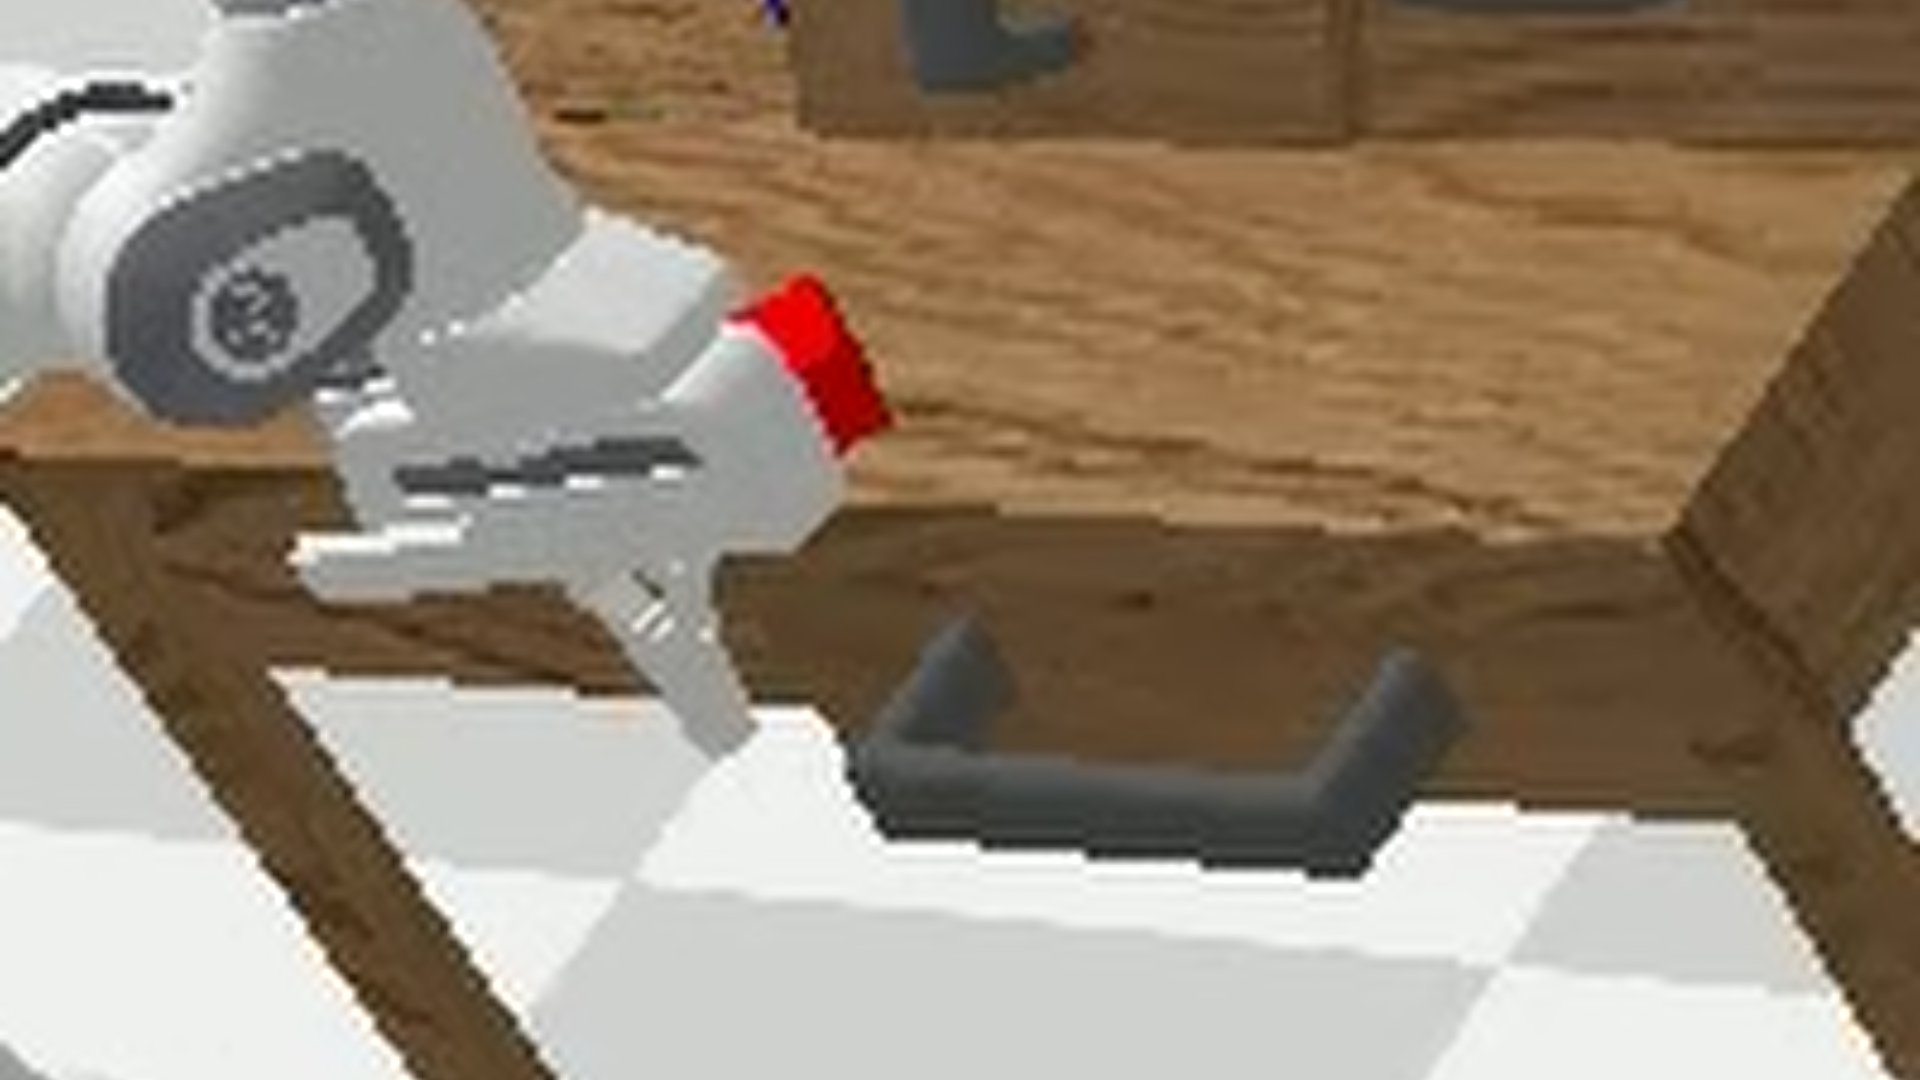
\includegraphics[width=0.24\linewidth]{figures/task2/fail_1.jpg}
    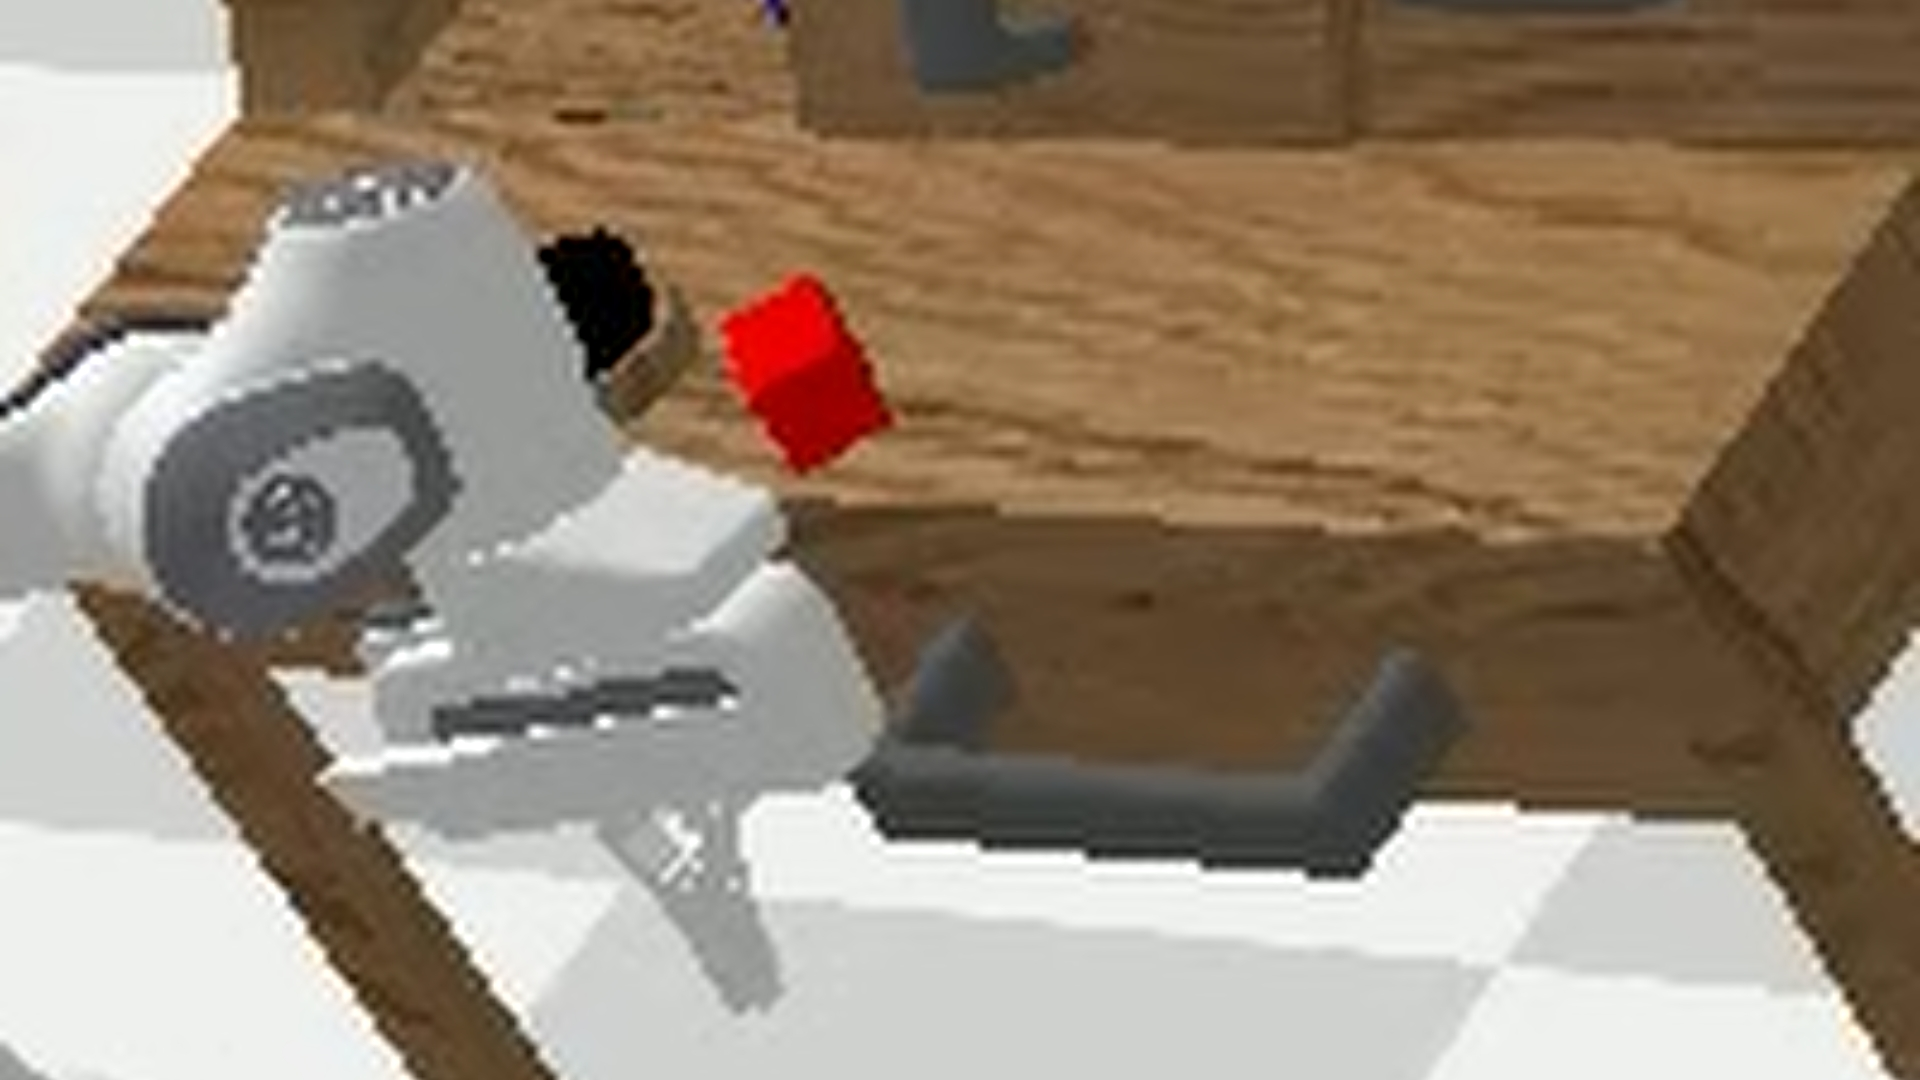
\includegraphics[width=0.24\linewidth]{figures/task2/fail_2.jpg}
    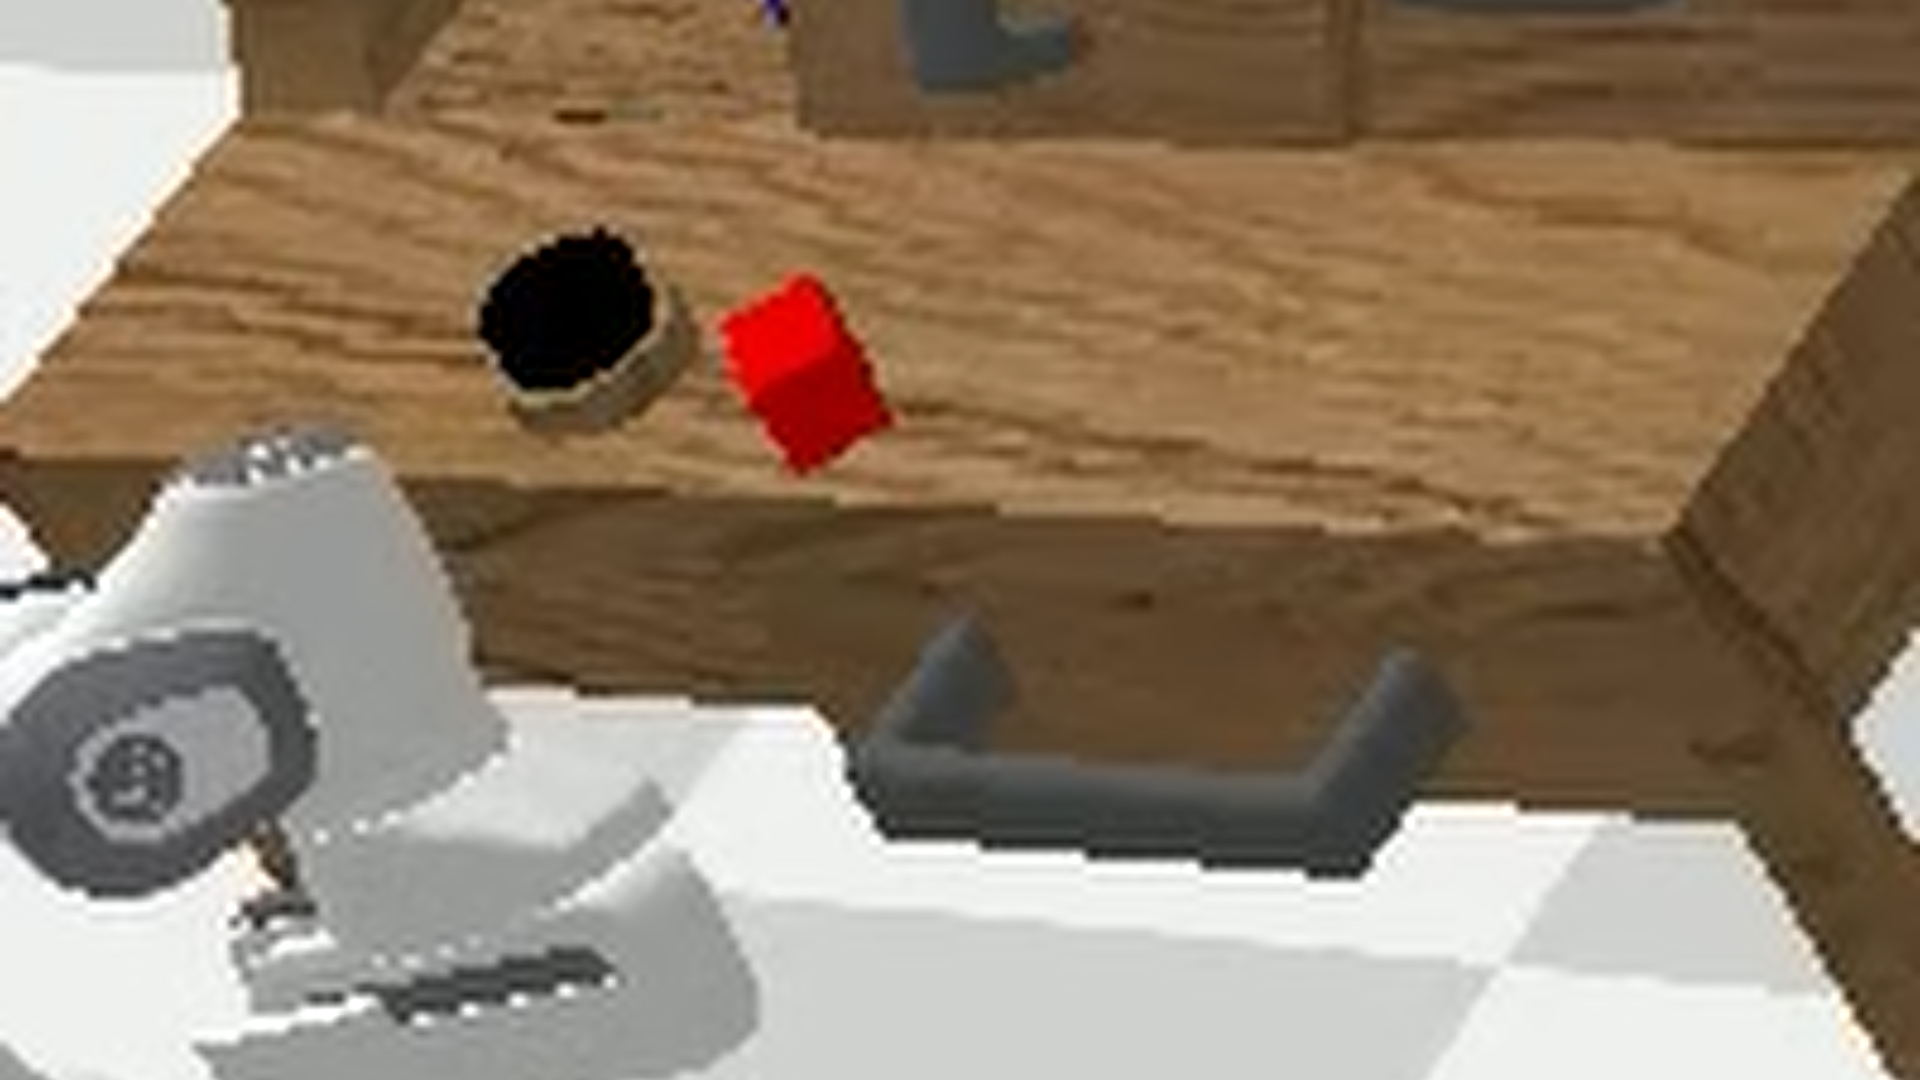
\includegraphics[width=0.24\linewidth]{figures/task2/fail_3.jpg}

    \vspace{0.5em}

    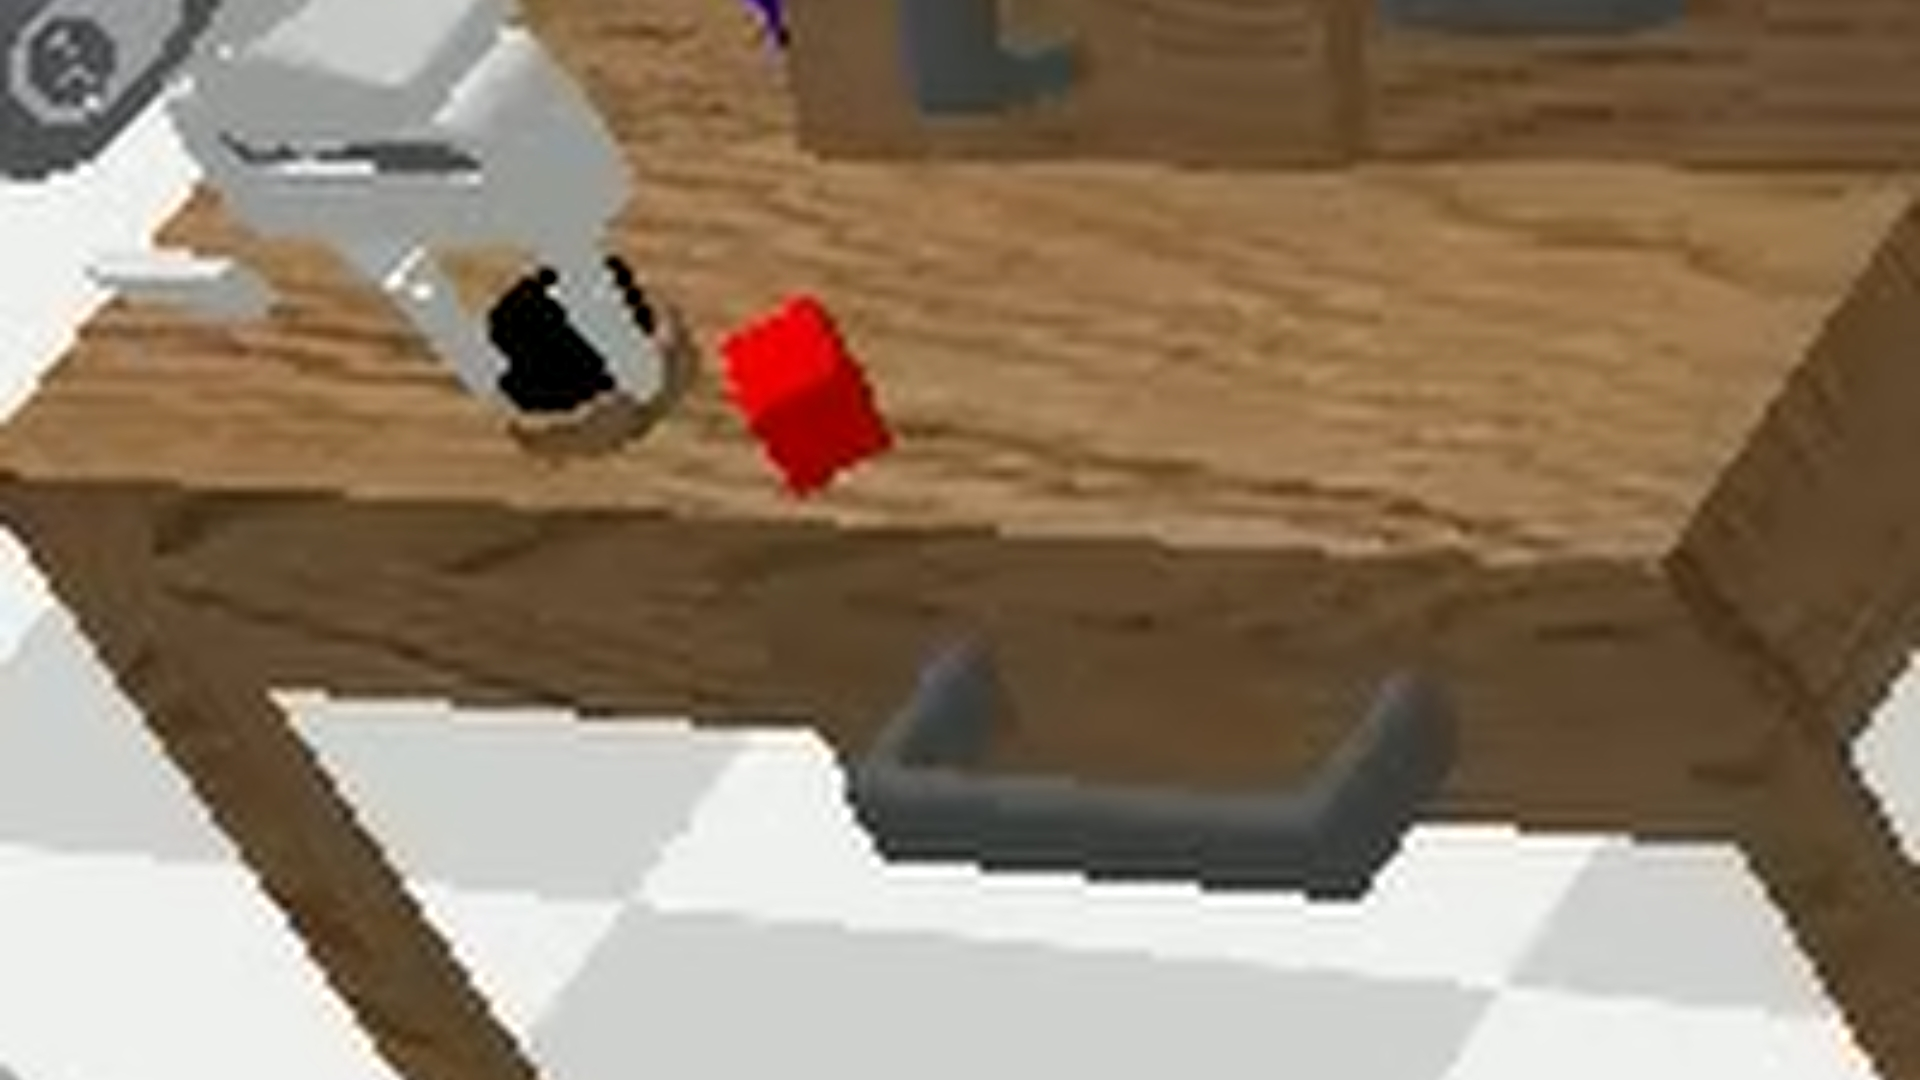
\includegraphics[width=0.24\linewidth]{figures/task2/success_0.jpg}
    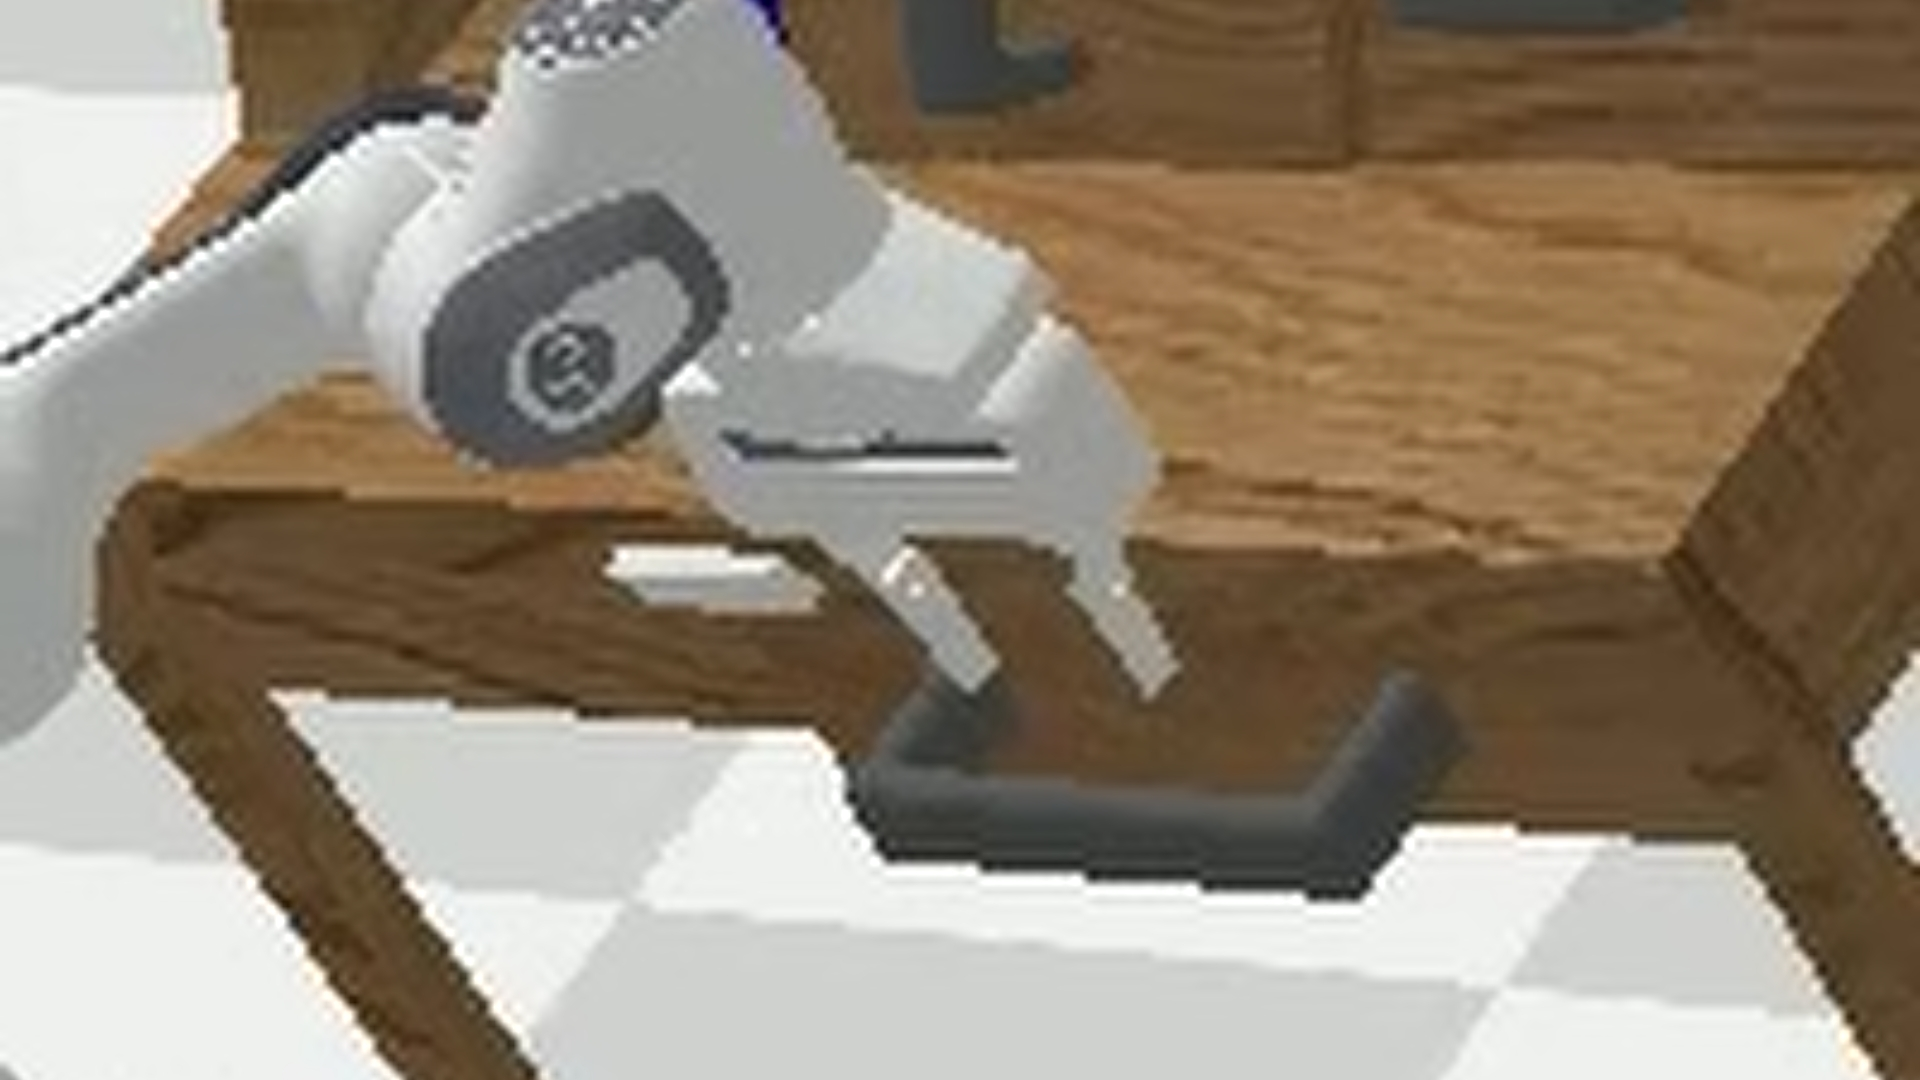
\includegraphics[width=0.24\linewidth]{figures/task2/success_1.jpg}
    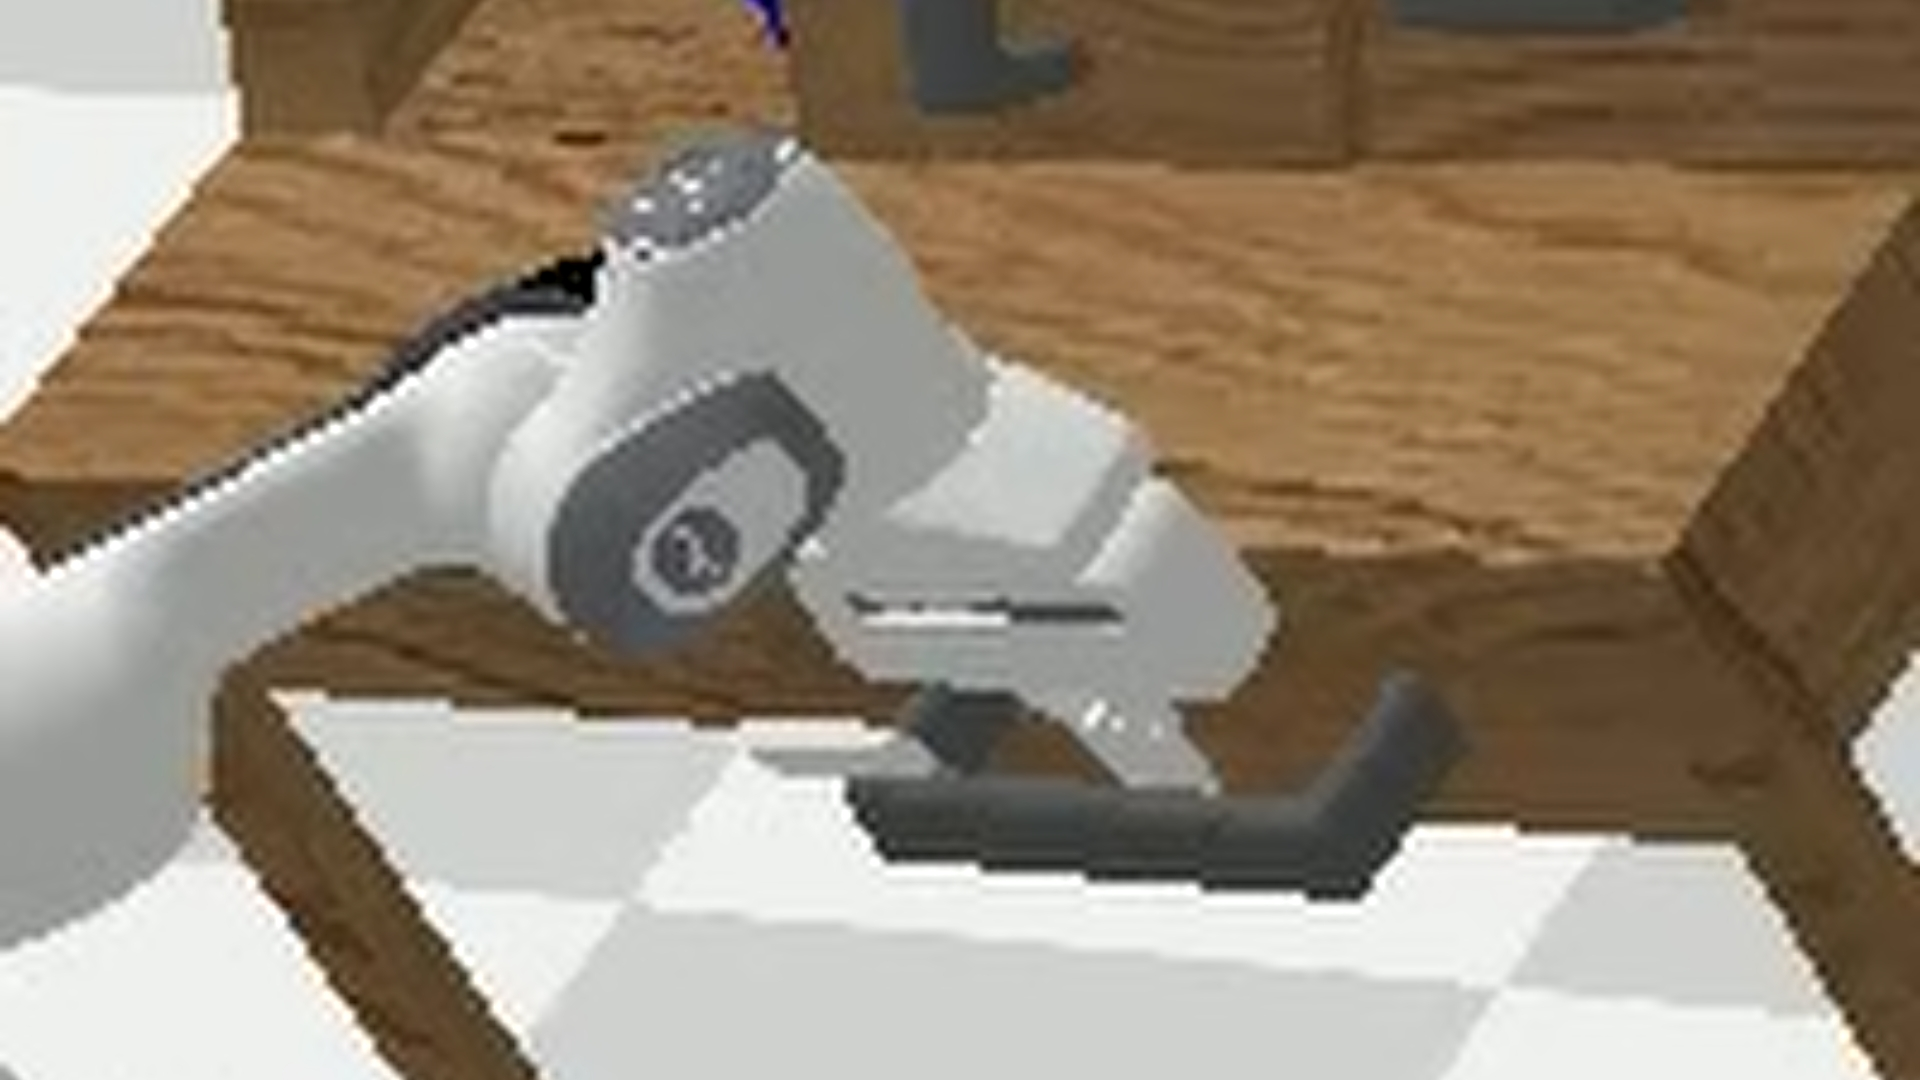
\includegraphics[width=0.24\linewidth]{figures/task2/success_2.jpg}
    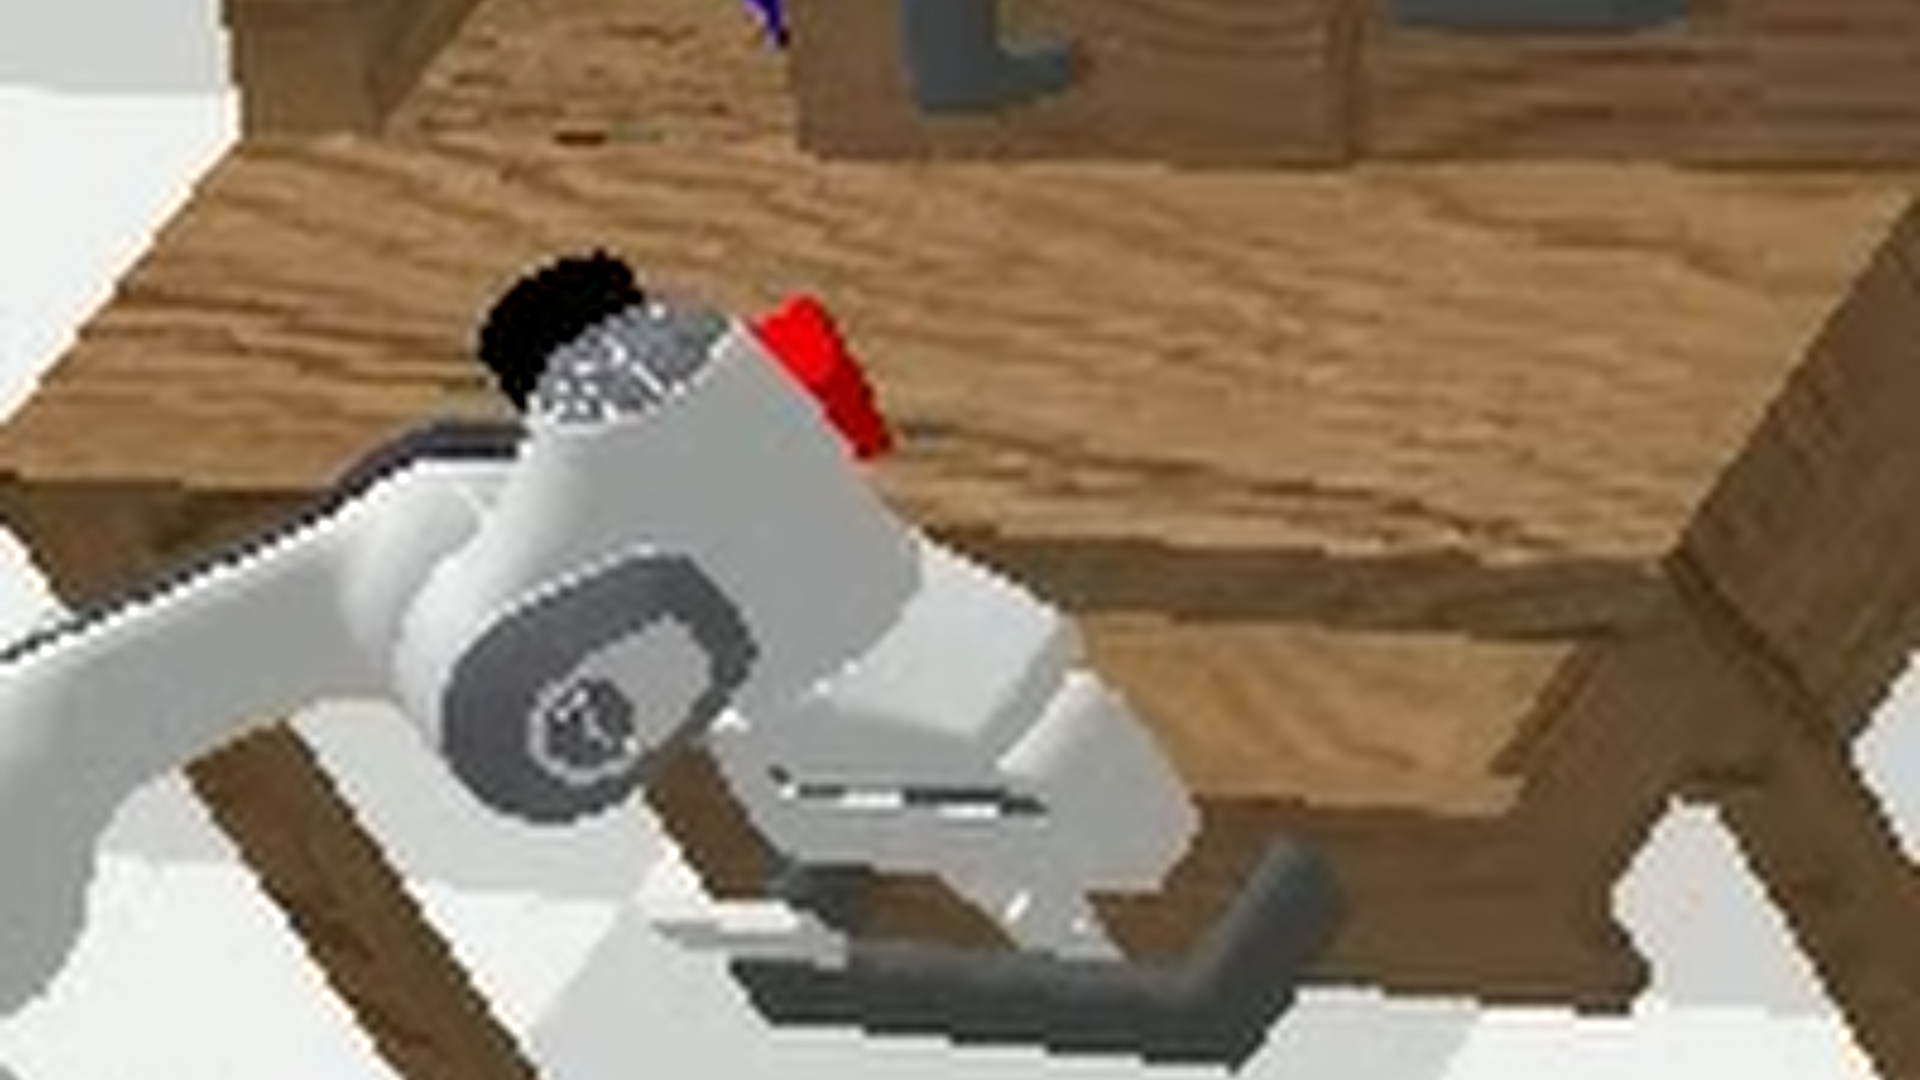
\includegraphics[width=0.24\linewidth]{figures/task2/success_3.jpg}

    \caption{Representative failed (top row) and successful (bottom row) open-drawer rollouts in Environment D. In both rollouts, the gripper approaches the drawer handle correctly, but successful execution requires accurate insertion of the gripper into the handle before the pulling motion.}
    \label{fig:open_drawer_success_failure}
\end{figure}

Overall, the results provide strong evidence that multi-environment training substantially improves robustness to visual distribution shifts. While both policies achieve similar action-level prediction accuracy, only the policy trained on multiple environments generalizes reliably to the unseen Environment D, achieving perfect task completion across all evaluation rollouts.

\subsection{Action Chunking Ablation Study}

To investigate the effect of ACT's action chunking mechanism, we conducted two complementary ablation studies. Specifically, we evaluated the influence of the action horizon on: (i) the Action $L_1$ Error using the full CALVIN dataset, and (ii) the rollout success rate on the \textit{Open Drawer} task subset.

\subsubsection{Evaluation Using Action L1 Error}

Table~\ref{tab} summarizes the Action L1 errors obtained with different action horizons. Figure~\ref{fig} visualizes the corresponding trend.

\begin{table}[h]
\centering
\caption{Effect of action horizon on Action L1 Error in the unseen environment D. Lower is better.}
\label{tab}
\begin{tabular}{c|ccccccc}
\hline
Model & 1 & 2 & 4 & 8 & 16 & 32 & 64 \\
\hline
B & 0.14841 & 0.14760 & \textbf{0.14346} & 0.14591 & 0.14528 & 0.14480 & 0.15069 \\
ABC & 0.12058 & 0.11974 & \textbf{0.11888} & 0.11961 & 0.11999 & 0.12073 & 0.12341 \\
\hline
\end{tabular}
\end{table}

\begin{figure}[h]
\centering
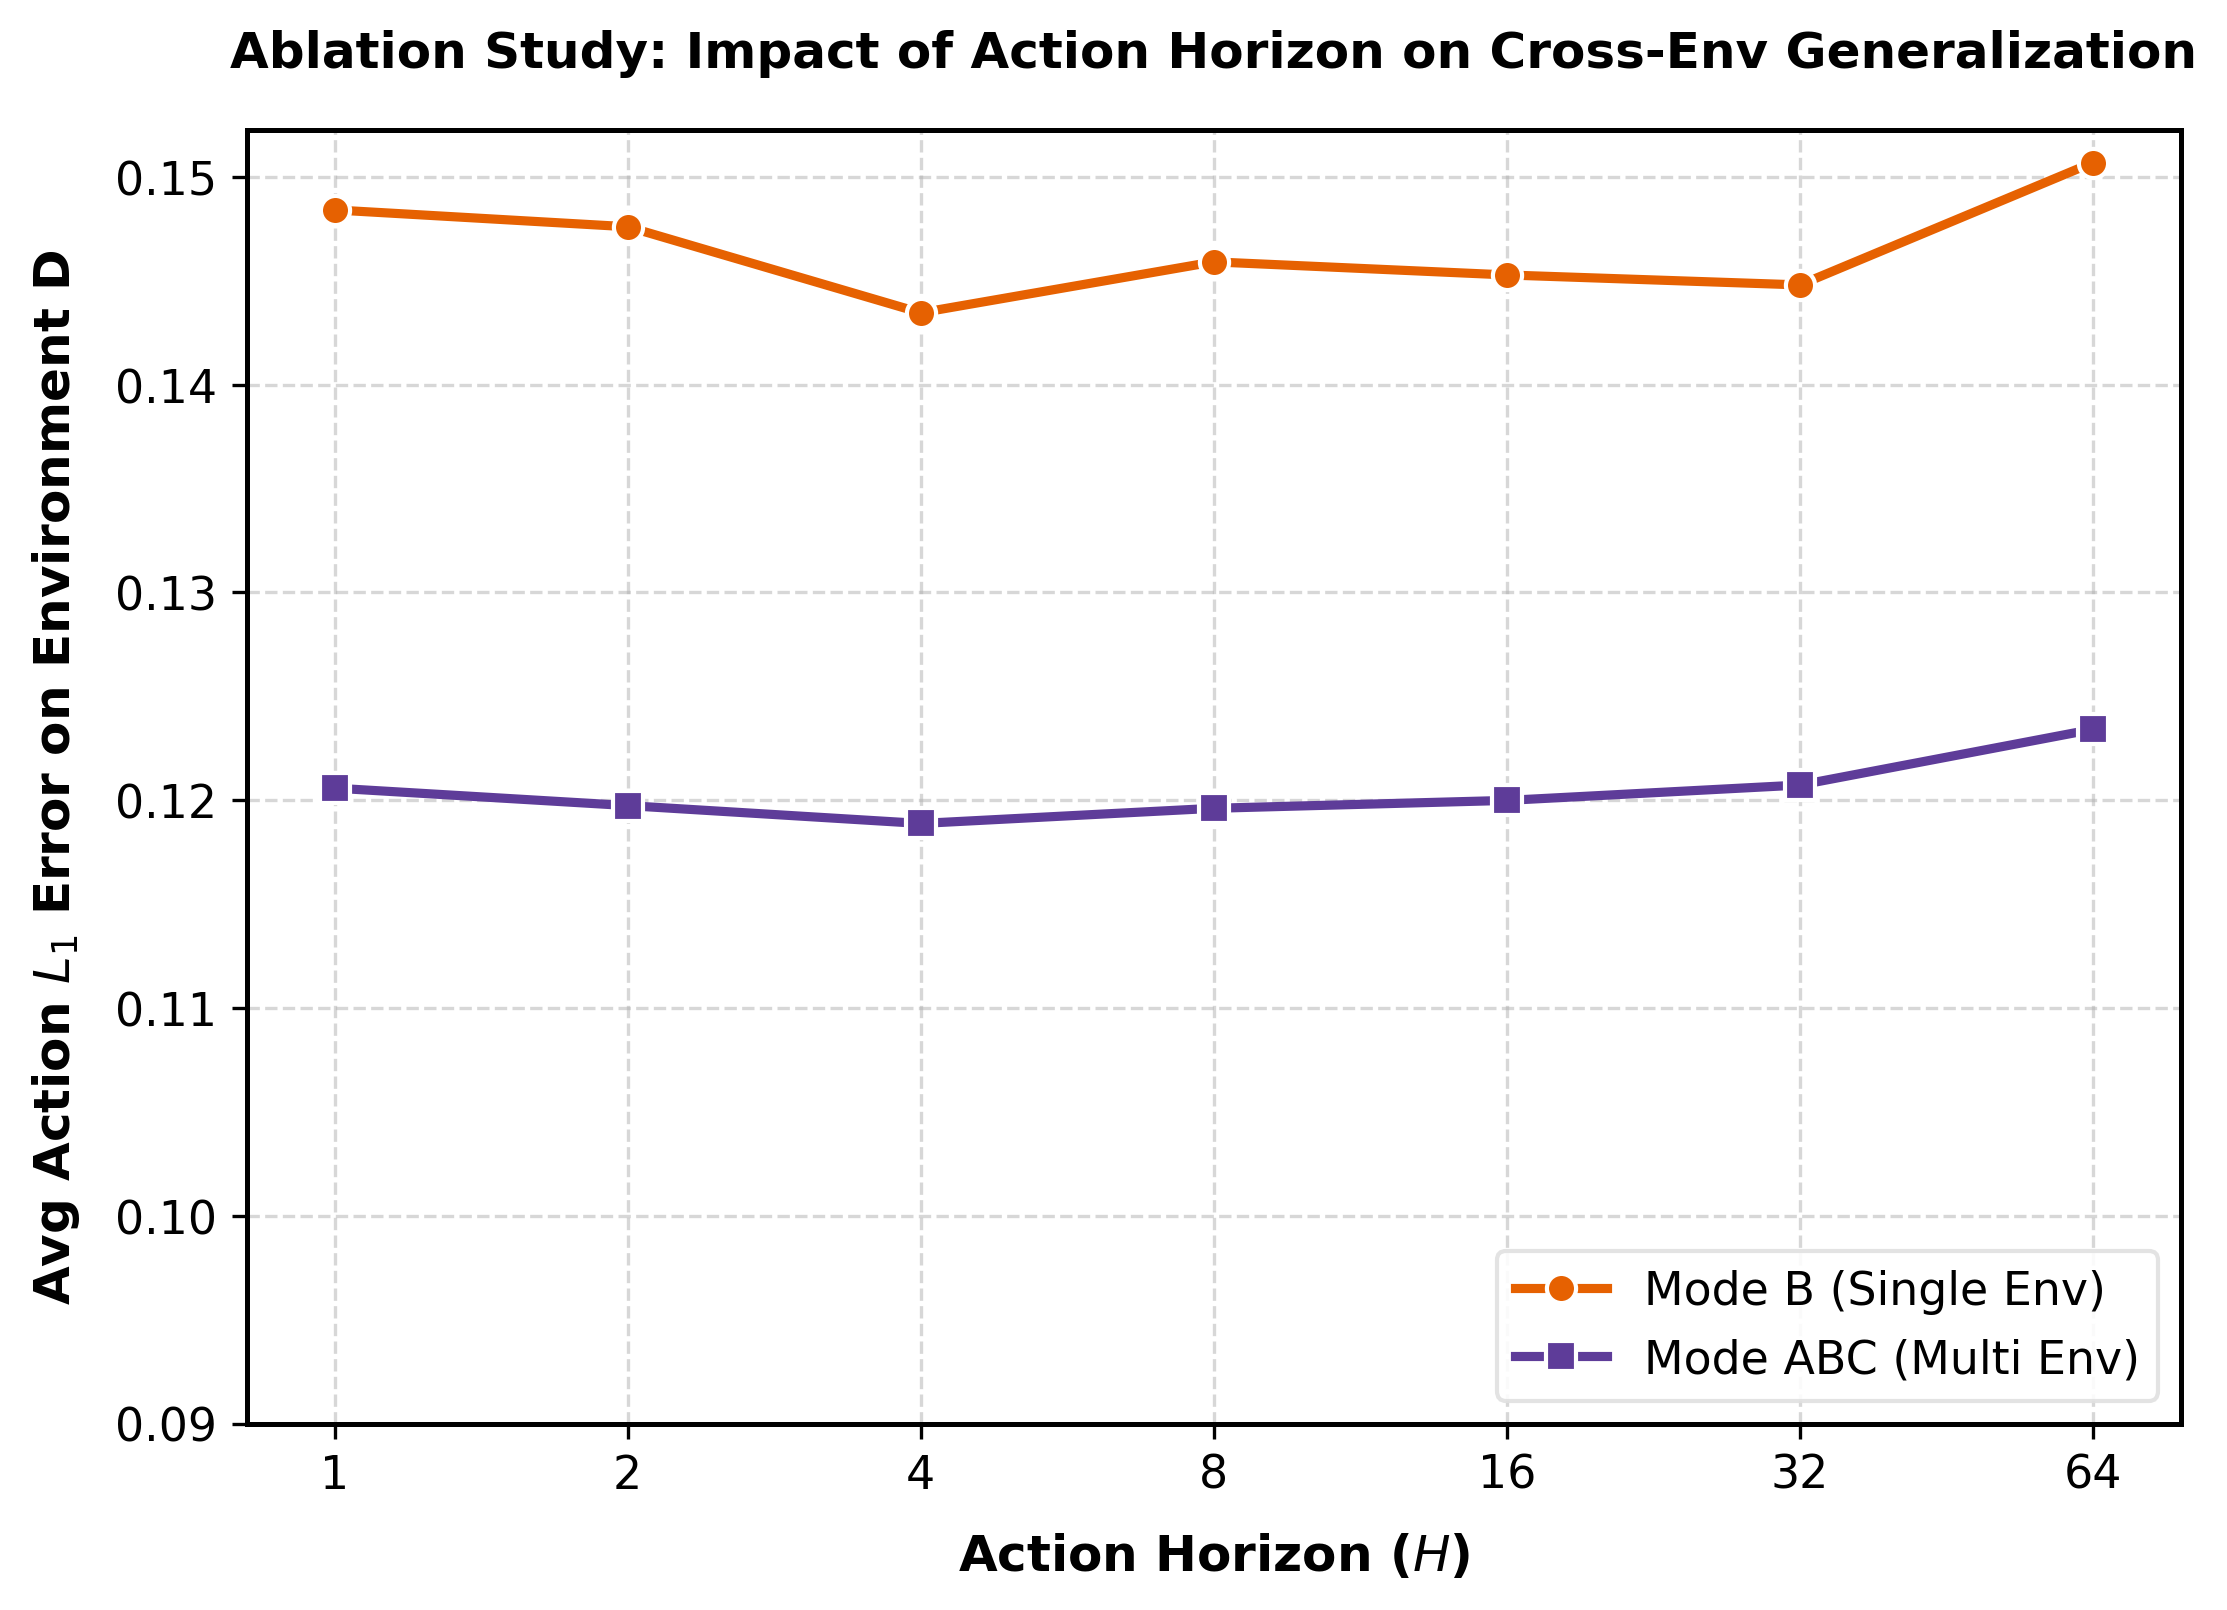
\includegraphics[width=0.75\linewidth]{figures/task2/horizon_ablation_curve.png}
\caption{Action L1 Error on environment D as a function of action horizon. Both the single-environment model (B) and the multi-environment model (ABC) achieve their lowest error at horizon $=4$.}
\label{fig}
\end{figure}

Several observations can be made from Figure~\ref{fig}. First, both models exhibit a remarkably similar trend despite being trained on different datasets. The Action L1 error decreases as the horizon increases from $1$ to $4$, reaches its minimum at horizon $=4$, and then gradually increases as the horizon becomes larger. This consistent behavior suggests that the optimal horizon is primarily determined by the temporal characteristics of the task rather than the amount of training data.

Second, the performance variation across different horizons is relatively moderate. Nevertheless, the best results are consistently obtained with horizon $=4$, yielding Action L1 errors of $0.14346$ and $0.11888$ for the B and ABC models, respectively. This indicates that a moderate chunk length provides a favorable balance between exploiting temporal correlations and maintaining prediction accuracy under visual distribution shifts.

\subsubsection{Evaluation Using Success Rate}

Additionally, we evaluated the influence of action horizon on an \textit{Open Drawer} subset using online simulation rollouts. For each horizon, 20 rollouts were executed and the task success rate was recorded.

\begin{table}[h]
\centering
\caption{Success rate on the Open Drawer subset under different action horizons.}
\label{tab:open_drawer_horizon}
\begin{tabular}{c|ccccc}
\hline
Horizon & 1 & 2 & 4 & 8 & 16 \\
\hline
Success Rate (\%) & 80 & 30 & \textbf{100} & \textbf{100} & 80 \\
\hline
\end{tabular}
\end{table}

Although the rollout budget is limited, the results are broadly consistent with the offline evaluation. Intermediate horizons ($4$ and $8$) achieve the highest success rates, whereas very small or large horizons result in inferior performance. Interestingly, horizon $=2$ performs substantially worse than all other settings. Given the limited number of rollouts, this phenomenon may be partially attributed to evaluation variance; nevertheless, it further suggests that excessively short action chunks do not fully exploit ACT's temporal modeling capability.

\subsubsection{Discussion: Robustness Under Visual Distribution Shift}

One of the key motivations behind ACT is that predicting a chunk of future actions can improve robustness by incorporating temporal consistency into the policy. The results of both ablation studies provide empirical evidence supporting this design choice.

When the action horizon is too small, the policy approaches a single-step predictor. Under visual distribution shifts, such a policy relies excessively on the immediate, potentially corrupted visual observation, making its predictions highly sensitive to observation noise and appearance variations. In contrast, training the policy to jointly predict a sequence of future actions acts as a strong regularizer. Even though only the first action of the chunk is executed in our setup, the multi-step prediction objective forces the network to capture underlying temporal structures and physical constraints. This reduces the policy's over-reliance on individual visual features at a single frame, thereby enhancing the stability of the executed action.

However, excessively large horizons introduce a different challenge. The policy must predict a long sequence of future actions from a single observation, increasing uncertainty and making long-term prediction errors more difficult to correct. Under unseen visual conditions, this over-extension can degrade the overall quality of the predicted chunk, including the first executed action.

Overall, the results suggest that ACT's action chunking mechanism improves robustness to visual distribution shifts when an appropriate horizon is chosen. For the CALVIN tasks considered in this work, a moderate horizon (approximately 4) provides the best balance between regularizing the action representation and minimizing prediction uncertainty, leading to the strongest cross-environment generalization performance.

\subsection{Additional Findings}

\subsubsection{Effect of EMA Action Aggregation}

In the original ACT framework, Exponential Moving Average (EMA) is typically used to smooth action predictions from overlapping chunks. To justify our choice of executing only the first action without EMA, we compare the non-EMA mode against the EMA mode across both offline prediction and online rollout performance. 

As shown in Table~\ref{tab:ema_comparison}, the non-EMA mode achieves a lower offline action $L_1$ error on Environment D. For online evaluation on the \textit{open drawer} task, both modes deliver an identical 100\% success rate. These results indicate that EMA does not provide performance benefits in our current setting, justifying its exclusion. However, we note that these validations are limited to relatively simple setups, and the potential advantages of EMA might still manifest in more complex scenarios.

\begin{table}[h]
\centering
\caption{Comparison between non-EMA and EMA inference modes.}
\label{tab:ema_comparison}
\begin{tabular}{lcc}
\hline
\textbf{Inference Mode} & \textbf{Avg. Action $L_1$ Error on D} & \textbf{\textit{Open Drawer} Success Rate on D} \\ \hline
First Action(ours)             & \textbf{0.14339}                      & 100.0\% (20/20)                                 \\
EMA ($k=0.1$)                        & 0.17151                  & 100.0\% (20/20)                  \\ \hline
\end{tabular}
\end{table}

\subsection{Limitations and Future Work}

Although the experimental results provide strong evidence that multi-environment training improves zero-shot cross-environment generalization, several limitations remain.

First, the success-rate evaluation is conducted only on the \textit{open drawer} task. While this task captures a representative manipulation scenario involving precise object interaction, it does not fully reflect the diversity of tasks available in the CALVIN benchmark. Future work could extend the evaluation to additional manipulation tasks such as button pressing, switch operation, and object transportation to obtain a more comprehensive assessment of cross-environment generalization.

Second, the ACT policies in this project are trained without language conditioning. Consequently, rollout-based evaluation on the full multi-task dataset is not feasible because the policy is not explicitly informed which task should be executed. To address this issue, we construct a task-specific dataset for online evaluation. However, this setting differs from the original CALVIN benchmark. Incorporating language instructions or other task-conditioning mechanisms would enable evaluation on the complete multi-task benchmark and provide a more realistic assessment of general-purpose manipulation policies.

Third, the current study focuses exclusively on visual distribution shifts between environments A--D. Although these environments exhibit substantial differences in appearance and object layouts, other forms of distribution shift remain unexplored, including sensor noise, lighting variations, camera perturbations, and changes in robot dynamics. Evaluating ACT under a broader range of domain shifts would provide deeper insights into its robustness.

Finally, our investigation of ACT's action chunking mechanism is limited to varying the action horizon while executing only the first predicted action at inference time. More sophisticated action aggregation strategies or adaptive horizon selection methods may further improve robustness and generalization performance.

Despite these limitations, the results consistently demonstrate that increasing environmental diversity during training is an effective strategy for improving zero-shot transfer. Future work along the directions outlined above may further enhance the robustness and practical applicability of imitation learning policies in unseen environments.

\subsection{Conclusion}

In this task, we evaluated the zero-shot cross-environment generalization of the ACT policy on the CALVIN benchmark. Our findings yield three key insights:

\begin{itemize}
    \item \textbf{Generalization in Action $L_1$ Loss:} While training solely on Environment B yields lower training loss, it heavily overfits to scene-specific visual features, causing the Action $L_1$ Error to deteriorate with prolonged training on the unseen Environment D. Conversely, multi-environment joint training (ABC) effectively regularizes the model against visual shifts, achieving a consistent $15.7\%$ relative reduction in offline prediction error.
    \item \textbf{Decisive Boost in Closed-Loop Success Rate:} The practical advantage of multi-environment training is most prominent when evaluated via rollout success rates. Under severe visual distribution shifts, the single-environment policy fails completely ($0\%$ success rate) as minor positioning errors compound during critical interaction phases. In contrast, the multi-environment policy achieves a flawless $100\%$ success rate, proving that diverse environmental exposure is paramount for robust task execution.
    \item \textbf{Empirical Sensitivity to Action Horizon:} The ablation study demonstrates that intermediate action horizons ($H=4$ and $H=8$) consistently deliver the best performance in both offline errors and online rollouts. This empirical trend suggests that a moderate chunk length strikes the best balance for the task; shorter or excessively long horizons both lead to performance degradation, potentially due to the trade-off between temporal consistency and long-term prediction uncertainty.
\end{itemize}

In conclusion, scaling environmental diversity during training combined with an empirically optimized action chunking horizon provides a effective framework for overcoming visual distribution shifts in embodied AI.


\appendix

\section{Project Resources}

\subsection{Task 1 Repository}

\url{https://github.com/F1shermanCNN/CV-Final-Task1}

\subsection{Task 1 Models, Blender Objects, and Rendering Videos}
\label{sec:models}
\url{https://drive.google.com/drive/folders/104ITdruMWy3bJy7J_qOayYOE7LNySR8B?usp=sharing}

\subsection{Task 2 Repository}

\url{https://github.com/Kevin-LD/lerobot-act-calvin}

\subsection{Task 2 Model Weights and Rollout Visualizations}

\url{https://drive.google.com/drive/folders/1UVtHY2a5legxZIZzB76gldc701c19pYH?usp=drive_link}

\subsection{Task 2 Complementary Dataset}

\url{https://huggingface.co/datasets/Kevin-LD/CALVIN_open_drawer/tree/main}

%\bibliographystyle{plainurl}
%\bibliographystyle{unsrt}
%\bibliography{refs.bib}

\end{document}
